%% ============================================================================
%% TCC — Pipeline Reprodutível para Montagem e Anotação de Mitogenomas
%% UERN — Universidade do Estado do Rio Grande do Norte
%% Autor: Matheus Sobreira Benevides
%% Formatação: Manual de Normalização UERN (3ª edição, 2022) + ABNT
%% ============================================================================

\documentclass[
    12pt,               % Tamanho da fonte (UERN: 12pt)
    openright,          % Capítulos iniciam em páginas ímpares
    oneside,            % Impressão apenas anverso (digital)
    a4paper,            % Tamanho do papel
    chapter=TITLE,      % Títulos de capítulo em maiúsculas
    section=TITLE,      % Seções primárias em maiúsculas
    english,            % Idioma secundário
    brazil,             % Idioma principal
    draft               % REMOVER para PDF final (acelera compilação)
]{abntex2}

% ---- Pacotes fundamentais ----
\usepackage[T1]{fontenc}
\usepackage[utf8]{inputenc}
\usepackage{mathptmx}           % Fonte Times New Roman (UERN)
\usepackage{lmodern}            % Evita fontes cm-super Type1 (acelera embed de ~25 fontes)
% microtype removido temporariamente (lento no Overleaf; adicionar de volta no PDF final)
\usepackage{indentfirst}        % Recuo na primeira linha de cada parágrafo

% ---- Pacotes de citação e referência (ABNT) ----
% backref removido temporariamente (lento; adicionar de volta no PDF final)
\usepackage[alf]{abntex2cite}   % Sistema autor-data ABNT

% ---- Pacotes adicionais ----
\usepackage{amsmath,amssymb}
\usepackage{graphicx}
\usepackage{booktabs}
\usepackage{longtable}
\usepackage{array}
\usepackage{float}
\usepackage{listings}
\usepackage{caption}
\usepackage{enumitem}
\usepackage{url}
\usepackage[left=3cm,top=3cm,right=2cm,bottom=2cm]{geometry}
% todonotes removido (carrega TikZ/PGF inteiro, lento no Overleaf)
\newcommand{\missingfigure}[2][]{{\centering\fbox{\parbox{0.8\textwidth}{\textit{[Figura pendente: #2]}}}\par}}

% ---- Configuração de espaçamento (UERN: 1,5 entre linhas) ----
\OnehalfSpacing

% ---- Configuração de recuo do parágrafo (UERN: 1,25 cm) ----
\setlength{\parindent}{1.25cm}

% ---- Tolerância para evitar Overfull \hbox menores ----
\setlength{\emergencystretch}{3em}

% ---- Configuração de listings para blocos de código ----
\lstset{
    basicstyle=\ttfamily\small,
    breaklines=true,
    frame=single,
    columns=fullflexible,
    keepspaces=true,
    showstringspaces=false,
    literate={á}{{\'a}}1 {é}{{\'e}}1 {í}{{\'i}}1 {ó}{{\'o}}1 {ú}{{\'u}}1
             {ã}{{\~a}}1 {õ}{{\~o}}1 {ç}{{\c{c}}}1
             {Á}{{\'A}}1 {É}{{\'E}}1 {Í}{{\'I}}1 {Ó}{{\'O}}1 {Ú}{{\'U}}1
             {Ã}{{\~A}}1 {Õ}{{\~O}}1 {Ç}{{\c{C}}}1
}

% backref config removida temporariamente (adicionar de volta no PDF final)
% \renewcommand{\backrefpagesname}{Citado na(s) página(s):~}
% \renewcommand{\backref}{}
% \renewcommand*{\backrefalt}[4]{
%     \ifcase #1
%         Nenhuma citação no texto.
%     \or
%         Citado na página #2.
%     \else
%         Citado #1 vezes nas páginas #2.
%     \fi
% }

% ---- Configuração de captions (UERN: fonte 10, alinhado à esquerda) ----
\captionsetup{
    font=small,
    justification=raggedright,
    singlelinecheck=false,
    labelsep=endash
}

% ---- Informações do documento ----
\titulo{Construção de um Pipeline Reprodutível para Montagem e Anotação Automatizada de Mitogenomas: Aplicação à Arara-azul-de-lear (\texorpdfstring{\textit{Anodorhynchus leari}}{Anodorhynchus leari})}
\autor{Matheus Sobreira Benevides}
\local{Mossoró}
\data{2025}
\orientador{Prof. Wilfredo}

\instituicao{%
    UNIVERSIDADE DO ESTADO DO RIO GRANDE DO NORTE
    \par
    FACULDADE DE CIÊNCIAS EXATAS E NATURAIS
    \par
    DEPARTAMENTO DE INFORMÁTICA
    \par
    CURSO DE CIÊNCIA DA COMPUTAÇÃO
}

\tipotrabalho{Monografia}
\preambulo{Monografia apresentada ao Curso de Ciência da Computação da Universidade do Estado do Rio Grande do Norte, como requisito parcial para obtenção do grau de Bacharel em Ciência da Computação.}

% ============================================================================
% INÍCIO DO DOCUMENTO
% ============================================================================
\begin{document}

% ---- Configuração do PDF (deve ficar após \begin{document}) ----
\hypersetup{
    pdftitle={Construção de um Pipeline Reprodutível para Montagem e Anotação Automatizada de Mitogenomas},
    pdfauthor={Matheus Sobreira Benevides},
    pdfsubject={Bioinformática -- Montagem de Mitogenomas},
    pdfkeywords={mitogenoma, pipeline, Nextflow, Docker, arara-azul-de-lear},
    colorlinks=true,
    linkcolor=black,
    citecolor=black,
    filecolor=black,
    urlcolor=blue,
    bookmarksdepth=2
}

% Seleciona o idioma principal
\selectlanguage{brazil}

% Retira espaço extra obsoleto entre frases
\frenchspacing

% ============================================================================
% ELEMENTOS PRÉ-TEXTUAIS
% ============================================================================
\pretextual

% ---- CAPA ----
\imprimircapa

% ---- FOLHA DE ROSTO ----
\imprimirfolhaderosto

% ---- FOLHA DE APROVAÇÃO ----
\begin{folhadeaprovacao}
    \begin{center}
        {\ABNTEXchapterfont\bfseries\MakeUppercase{\imprimirautor}}
        \vspace*{1cm}

        {\ABNTEXchapterfont\bfseries\MakeUppercase{\imprimirtitulo}}
        \vspace*{1cm}
    \end{center}

    \hfill
    \begin{minipage}{0.55\textwidth}
        \SingleSpacing
        \imprimirpreambulo
    \end{minipage}

    \vspace*{1cm}

    Aprovada em: \_\_\_\_/\_\_\_\_/\_\_\_\_\_\_\_\_.

    \vspace*{1cm}
    \begin{center}
        \textbf{Banca examinadora}
    \end{center}

    \vspace*{1cm}
    \assinatura{Prof. Wilfredo (Orientador) \\ Universidade do Estado do Rio Grande do Norte -- UERN}
    \assinatura{Prof. Carlos \\ Universidade do Estado do Rio Grande do Norte -- UERN}
    \assinatura{Prof. Bruno \\ Universidade do Estado do Rio Grande do Norte -- UERN}
\end{folhadeaprovacao}

% ---- DEDICATÓRIA (opcional) ----
% \begin{dedicatoria}
%     \vspace*{\fill}
%     \hspace{8cm}
%     \begin{minipage}{\dimexpr\textwidth-8cm}
%         Texto da dedicatória.
%     \end{minipage}
% \end{dedicatoria}

% ---- AGRADECIMENTOS (opcional) ----
% \begin{agradecimentos}
%     Texto dos agradecimentos.
% \end{agradecimentos}

% ---- EPÍGRAFE (opcional) ----
% \begin{epigrafe}
%     \vspace*{\fill}
%     \hspace{8cm}
%     \begin{minipage}{\dimexpr\textwidth-8cm}
%         ``Texto da epígrafe.'' (AUTOR, ano, p. X).
%     \end{minipage}
% \end{epigrafe}

% ---- RESUMO ----
\begin{resumo}
    Este trabalho apresenta o desenvolvimento e a validação de um pipeline de bioinformática automatizado, reprodutível e portável para a montagem \textit{de novo} e anotação funcional de genomas mitocondriais, utilizando tecnologias de conteinerização (Docker) e sistemas de gerenciamento de \textit{workflows} (Nextflow DSL2). O pipeline integra sete etapas sequenciais --- análise piloto de qualidade, aquisição de dados do NCBI SRA, controle de qualidade com FastQC, remoção de adaptadores com Trim Galore, montagem com NOVOPlasty, anotação funcional com MITOS2 e compilação automática de 14 categorias de entregáveis, incluindo arquivos em formato GenBank Flat File prontos para submissão. A validação foi realizada com duas espécies: \textit{Diploprion bifasciatus} (Perciformes), como espécie-controle, e a arara-azul-de-lear (\textit{Anodorhynchus leari}, Psittaciformes), como espécie-alvo. O mitogenoma da arara-azul-de-lear foi reconstruído com 16.986 pares de bases circularizados, cobertura de 306$\times$ e o conjunto completo de 37 genes (13 CDS, 22 tRNAs, 2 rRNAs), diferindo em apenas 13 bp do congênere \textit{A. hyacinthinus}. O módulo Pilot QC, juntamente com estratégias de truncamento adaptativo, permitiu reduzir o volume de dados em aproximadamente 5 milhões de vezes (de 87 GB para 17 KB), viabilizando a execução completa em um notebook com 16 GB de RAM em menos de uma hora. O pipeline e o código-fonte estão disponíveis em repositório público no GitHub, como contribuição à ciência aberta e à conservação da biodiversidade brasileira.

    \vspace{\onelineskip}
    \noindent
    \textbf{Palavras-chave}: mitogenoma; pipeline; bioinformática; reprodutibilidade; Nextflow; Docker; arara-azul-de-lear.
\end{resumo}

% ---- ABSTRACT ----
\begin{resumo}[Abstract]
    \begin{otherlanguage*}{english}
        This work presents the development and validation of an automated, reproducible and portable bioinformatics pipeline for \textit{de novo} assembly and functional annotation of mitochondrial genomes, using containerization technologies (Docker) and workflow management systems (Nextflow DSL2). The pipeline integrates seven sequential stages --- pilot quality analysis, NCBI SRA data acquisition, quality control with FastQC, adapter removal with Trim Galore, assembly with NOVOPlasty, functional annotation with MITOS2, and automatic compilation of 14 deliverable categories, including GenBank Flat File format files ready for submission. Validation was performed with two species: \textit{Diploprion bifasciatus} (Perciformes), as a control species, and the Lear's Macaw (\textit{Anodorhynchus leari}, Psittaciformes), as the target species. The Lear's Macaw mitogenome was reconstructed with 16,986 circularized base pairs, 306$\times$ coverage and the complete set of 37 genes (13 CDS, 22 tRNAs, 2 rRNAs), differing by only 13 bp from the congeneric \textit{A. hyacinthinus}. The Pilot QC module, combined with adaptive truncation strategies, reduced the data volume by approximately 5 million times (from 87 GB to 17 KB), enabling complete execution on a notebook with 16 GB of RAM in under one hour. The pipeline and source code are available in a public GitHub repository, as a contribution to open science and the conservation of Brazilian biodiversity.

        \vspace{\onelineskip}
        \noindent
        \textbf{Keywords}: mitogenome; pipeline; bioinformatics; reproducibility; Nextflow; Docker; Lear's Macaw.
    \end{otherlanguage*}
\end{resumo}

% ---- LISTA DE ILUSTRAÇÕES (opcional) ----
% \pdfbookmark[0]{\listfigurename}{lof}
% \listoffigures*
% \cleardoublepage

% ---- LISTA DE TABELAS (opcional) ----
% \pdfbookmark[0]{\listtablename}{lot}
% \listoftables*
% \cleardoublepage

% ---- LISTA DE ABREVIATURAS E SIGLAS ----
\begin{siglas}
    \item[ABNT] Associação Brasileira de Normas Técnicas
    \item[bp] Pares de bases (\textit{base pairs})
    \item[CDS] Sequência codificante (\textit{Coding Sequence})
    \item[DNA] Ácido desoxirribonucleico
    \item[FAIR] \textit{Findable, Accessible, Interoperable, and Reusable}
    \item[GFF] \textit{General Feature Format}
    \item[HPC] Computação de Alto Desempenho (\textit{High Performance Computing})
    \item[IUCN] União Internacional para a Conservação da Natureza
    \item[mRNA] RNA mensageiro
    \item[mtDNA] DNA mitocondrial
    \item[NCBI] \textit{National Center for Biotechnology Information}
    \item[NGS] Sequenciamento de Nova Geração (\textit{Next-Generation Sequencing})
    \item[ORF] Quadro aberto de leitura (\textit{Open Reading Frame})
    \item[RNA] Ácido ribonucleico
    \item[rRNA] RNA ribossomal
    \item[RSCU] \textit{Relative Synonymous Codon Usage}
    \item[SRA] \textit{Sequence Read Archive}
    \item[tRNA] RNA transportador
\end{siglas}

% ---- SUMÁRIO ----
\pdfbookmark[0]{\contentsname}{toc}
\tableofcontents*
\cleardoublepage

% ============================================================================
% ELEMENTOS TEXTUAIS
% ============================================================================
\textual

% Para compilar apenas um capítulo no Overleaf (descomente e ajuste):
% \includeonly{capitulos/cap6-mitogenoma}

% ============================================================================
% CAPÍTULO 1 — INTRODUÇÃO
% ============================================================================

\chapter{Introdução}

\section{Contextualização e Tema}

Os genomas mitocondriais --- também denominados \textbf{mitogenomas} --- constituem o conjunto completo de material genético contido na mitocôndria, \textbf{organela} (estrutura subcelular com função especializada) responsável pela produção de energia nas \textbf{células eucarióticas} (células que possuem núcleo delimitado por membrana --- categoria que inclui animais, plantas e fungos, em oposição às bactérias). Essas moléculas de DNA ocupam uma posição central na biologia evolutiva, genética de populações e sistemática, uma vez que oferecem informações valiosas sobre parentesco, variação intra e interespecífica e processos de conservação. O DNA mitocondrial, por suas características estruturais e funcionais --- como a \textbf{herança predominantemente materna} (transmissão exclusiva pela linhagem feminina, sem contribuição paterna), a ausência de \textbf{recombinação} (processo em que \textbf{cromossomos}, as estruturas lineares de DNA no núcleo celular, trocam segmentos durante a reprodução sexual --- ausente no mtDNA, cada molécula é uma cópia integral da mãe) e a elevada taxa evolutiva em comparação ao DNA nuclear ---, tornou-se um marcador molecular amplamente utilizado em diferentes contextos biológicos \cite{boore1999,ekblom2014}.

O avanço das tecnologias de sequenciamento de nova geração (\textit{Next-Generation Sequencing} --- NGS) ampliou o acesso a grandes volumes de dados, favorecendo a obtenção de mitogenomas completos e de alta qualidade. No entanto, a reconstrução dessas moléculas a partir de dados brutos permanece um desafio técnico, especialmente no caso de \textbf{leituras curtas} (\textit{reads} --- os fragmentos individuais de sequência de DNA produzidos pelo sequenciador, tipicamente com 100 a 300 pares de bases), que exigem algoritmos sofisticados para superar problemas como regiões repetitivas e possíveis falhas de \textbf{montagem} --- o processo computacional de reconstruir a sequência original do genoma a partir desses fragmentos sobrepostos. Nesse cenário, ferramentas especializadas, como o NOVOPlasty, têm desempenhado papel fundamental ao implementar estratégias de \textit{seed-and-extend} capazes de recuperar organelas de forma eficiente a partir de dados de genoma total \cite{dierckxsens2017}.

Embora a diversidade de softwares tenha contribuído para avanços significativos na montagem de organelas, a ausência de padronização metodológica ainda compromete a reprodutibilidade das análises. A multiplicidade de versões, dependências e configurações de ambiente gera obstáculos práticos para replicar experimentos, fenômeno amplamente conhecido como \textit{dependency hell} \cite{gruning2018}. Esse problema se insere no contexto mais amplo da crise de reprodutibilidade científica \cite{baker2016}, que tem motivado a adoção, na bioinformática, de práticas da engenharia de software, como a conteinerização de ambientes computacionais com Docker \cite{merkel2014} e a orquestração de fluxos com sistemas de gerenciamento de workflows, a exemplo do Nextflow \cite{ditommaso2017}.

Além da montagem propriamente dita, a anotação funcional dos genes mitocondriais constitui uma etapa igualmente relevante, que permite identificar os genes codificadores de proteínas, RNAs transportadores e RNAs ribossômicos presentes na molécula reconstruída. Ferramentas como o MITOS2 \cite{donath2019} automatizam essa tarefa, mas sua execução --- normalmente restrita a interfaces web --- permanece desvinculada dos pipelines de montagem, criando uma descontinuidade no fluxo analítico.

Soma-se a esses desafios computacionais uma barreira de infraestrutura frequentemente subestimada. Datasets de sequenciamento de genoma total alcançam dezenas a centenas de gigabytes --- o dataset da arara-azul-de-lear (\textit{Anodorhynchus leari}) utilizado neste trabalho, por exemplo, totaliza 87 GB em formato FASTQ descomprimido. Processar esse volume na íntegra exigiria centenas de gigabytes de armazenamento temporário e memória RAM proporcional, recursos indisponíveis em computadores pessoais típicos de estudantes e pequenos laboratórios. Sem estratégias inteligentes de redução de dados, a montagem de mitogenomas a partir de dados públicos ficaria restrita a grupos com acesso a servidores dedicados.

\section{Problema de Pesquisa}

Diante do cenário apresentado --- marcado pela fragmentação das ferramentas de montagem e anotação, pela ausência de padronização metodológica que compromete a reprodutibilidade, pela desconexão entre etapas analíticas que obriga o uso de interfaces web manuais, e pela barreira computacional imposta pelo volume dos dados de sequenciamento ---, este trabalho busca responder à seguinte questão:

\textbf{De que maneira é possível integrar, em um único fluxo de trabalho automatizado, as etapas de aquisição, controle de qualidade, montagem \textit{de novo}, anotação funcional e preparação para submissão ao GenBank de genomas mitocondriais, garantindo reprodutibilidade, portabilidade e viabilidade computacional em hardware doméstico?}

\section{Objetivos}

\subsection{Objetivo Geral}

Desenvolver e validar um pipeline de bioinformática automatizado, reprodutível e portável para a montagem \textit{de novo} e anotação funcional de genomas mitocondriais, utilizando tecnologias de conteinerização (Docker) e sistemas de gerenciamento de workflows (Nextflow).

\subsection{Objetivos Específicos}

\begin{enumerate}[label=\alph*)]
    \item Containerizar, por meio de Dockerfiles com versões pinadas, cada uma das ferramentas bioinformáticas necessárias ao pipeline (SRA-Toolkit, FastQC, Trim Galore, NOVOPlasty e MITOS2).
    \item Desenvolver o script de orquestração do pipeline utilizando Nextflow DSL2, definindo os processos, suas entradas, saídas e interdependências em módulos independentes.
    \item Integrar os containers Docker ao workflow, garantindo que cada etapa da análise seja executada em seu próprio ambiente isolado e pré-configurado.
    \item Implementar um módulo de análise piloto de qualidade (Pilot QC) capaz de determinar automaticamente o volume ideal de dados a serem processados, com base na qualidade das leituras e na fração mitocondrial estimada.
    \item Integrar a anotação funcional automatizada (MITOS2) ao pipeline, incluindo a geração de estruturas secundárias de tRNAs e rRNAs via ViennaRNA.
    \item Automatizar a geração de entregáveis em formato GenBank Flat File, com tratamento adequado de particularidades gênicas como o \textit{frameshift} do ND3 em aves.
    \item Validar o pipeline automatizado por meio de estudos de caso com dados públicos de sequenciamento de pelo menos duas espécies de grupos \textbf{taxonômicos} distintos --- isto é, de posições diferentes na classificação biológica hierárquica (espécie, gênero, família, ordem, etc.) ---, comparando os genomas montados e anotados com resultados de referência.
    \item Disponibilizar o pipeline completo e sua documentação em repositório público no GitHub, assegurando sua acessibilidade e reprodutibilidade pela comunidade científica.
\end{enumerate}

\section{Justificativa}

A análise de mitogenomas representa um componente essencial para a biologia evolutiva, a genética de populações e a sistemática, dado que essas moléculas fornecem informações relevantes sobre relações de parentesco, variação intra e interespecífica e processos de conservação. Sua relevância científica foi consolidada em trabalhos seminais que destacaram o papel estrutural e evolutivo dos mitogenomas como marcadores moleculares \cite{boore1999}, em estudos que enfatizaram sua aplicabilidade em investigações de genética de populações e evolução molecular \cite{ekblom2014} e em contribuições mais recentes que demonstraram seu potencial em análises de biodiversidade e conservação por meio de avanços metodológicos em montagem e anotação de organelas \cite{ulianosilva2023}.

Embora a obtenção de mitogenomas completos tenha sido amplamente favorecida pelo advento do NGS, a execução de pipelines de montagem ainda enfrenta desafios técnicos significativos. A diversidade de ferramentas, versões e dependências envolvidas gera um cenário de difícil replicação, conhecido como \textit{dependency hell}, que compromete a reprodutibilidade e a padronização das análises \cite{sandve2013,baker2016,gruning2018}.

Esse problema se torna especialmente relevante quando aplicado ao estudo de espécies ameaçadas de extinção, nas quais a disponibilidade de amostras biológicas é limitada e a confiabilidade dos resultados genômicos é crucial para fundamentar decisões de conservação. É o caso da \textbf{arara-azul-de-lear} (\textit{Anodorhynchus leari}), ave endêmica da Caatinga nordestina do Brasil, classificada como ``Em Perigo'' pela IUCN Red List. Com população estimada em pouco mais de 1.700 indivíduos na natureza \cite{icmbio2022}, a espécie depende de dados genômicos acessíveis e validáveis para subsidiar programas de manejo, reprodução em cativeiro e monitoramento populacional. Embora seu mitogenoma já tenha sido previamente reconstruído em atividade acadêmica, essa montagem foi realizada de forma manual, sem padronização metodológica e sem disponibilização pública do fluxo de trabalho --- o que impede sua verificação e replicação por outros pesquisadores.

Um desafio adicional reside na completude dos pipelines existentes. A maioria das ferramentas e workflows publicados concentra-se exclusivamente na etapa de montagem, sem integrar a anotação funcional nem a preparação dos resultados para submissão a bancos de dados públicos como o GenBank. Essa lacuna obriga o pesquisador a recorrer a interfaces web externas (e.g., MITOS2 via UseGalaxy) e a conversões manuais de formato, introduzindo etapas não rastreáveis que comprometem a reprodutibilidade do ciclo completo de análise.

Nesse contexto, torna-se necessário o desenvolvimento de soluções que conciliem robustez biológica, consistência computacional e acessibilidade de hardware. A adoção de práticas modernas da engenharia de software, como a containerização e os sistemas de gerenciamento de workflows, tem se mostrado fundamental para superar limitações de reprodutibilidade, além de permitir que fluxos analíticos sejam portáveis, escaláveis e transparentes \cite{ditommaso2017,ewels2020}.

Assim, este trabalho justifica-se pela proposta de construir um pipeline automatizado e reprodutível que cubra o ciclo completo --- desde a aquisição dos dados brutos até a geração de arquivos prontos para submissão ao GenBank (banco de dados público mantido pelo NCBI para depósito de sequências genéticas) ---, unindo boas práticas de ciência aberta e engenharia computacional à relevância biológica dos mitogenomas. A aplicação ao caso concreto da arara-azul-de-lear demonstra não apenas a viabilidade técnica da abordagem, mas também sua contribuição direta para a conservação de uma espécie ameaçada da biodiversidade brasileira.

\section{Metodologia}

O presente trabalho adota uma abordagem de pesquisa aplicada, de natureza experimental, com desenvolvimento iterativo e incremental de software. O pipeline foi implementado em Nextflow DSL2 e containerizado com Docker, seguindo boas práticas de engenharia de software científico \cite{wilson2014}.

A validação foi realizada por meio de dois estudos de caso com dados públicos do NCBI Sequence Read Archive (SRA): (i) \textit{Diploprion bifasciatus} (Perciformes --- peixe-sabão barrado), como espécie-controle para verificação funcional do pipeline; e (ii) arara-azul-de-lear (\textit{Anodorhynchus leari}, Psittaciformes --- aves), como espécie-alvo para a aplicação final. Em ambos os casos, os mitogenomas foram montados \textit{de novo} a partir de leituras Illumina de genoma total e comparados com referências disponíveis no GenBank.

O pipeline integra sete etapas sequenciais automatizadas: (1) análise piloto de qualidade para dimensionamento do volume de dados; (2) download e truncamento dos dados do SRA; (3) controle de qualidade com FastQC; (4) remoção de adaptadores e bases de baixa qualidade com Trim Galore; (5) montagem \textit{de novo} com NOVOPlasty; (6) anotação funcional com MITOS2; e (7) compilação automática de 14 categorias de entregáveis, incluindo arquivos em formato GenBank Flat File prontos para submissão. Os detalhes de cada etapa, incluindo ferramentas, parâmetros e versões utilizadas, são apresentados no Capítulo~\ref{cap:metodologia}.

\section{Estrutura do Trabalho}

O presente trabalho está organizado em sete capítulos. Este primeiro capítulo apresentou a contextualização do tema, o problema de pesquisa, os objetivos, a justificativa e um breve resumo metodológico.

O \textbf{Capítulo~\ref{cap:referencial}} reúne o referencial teórico, abordando os fundamentos da montagem \textit{de novo} de genomas, as especificidades do DNA mitocondrial, a crise de reprodutibilidade em ciência computacional, a tecnologia de conteinerização com Docker e os sistemas de gerenciamento de workflows científicos.

O \textbf{Capítulo~\ref{cap:trabalhos}} analisa os trabalhos relacionados, revisando as principais ferramentas disponíveis para montagem de organelas --- MitoHiFi, MITObim, GetOrganelle, MToolBox e NOVOPlasty --- e apresenta uma análise comparativa entre elas.

O \textbf{Capítulo~\ref{cap:metodologia}} detalha a metodologia, descrevendo o processo de desenvolvimento de software adotado, a visão geral e o fluxo de execução do pipeline, sua arquitetura modular, as ferramentas e tecnologias utilizadas, e cada uma das sete etapas da análise.

O \textbf{Capítulo~\ref{cap:resultados}} apresenta os resultados obtidos nas execuções do pipeline e a discussão, incluindo as métricas de montagem e anotação para ambas as espécies, a análise de desempenho computacional e uma avaliação da robustez da abordagem.

O \textbf{Capítulo~\ref{cap:mitogenoma}} é dedicado integralmente à arara-azul-de-lear, apresentando a caracterização detalhada de seu mitogenoma, a análise dos genes codificadores de proteínas, RNAs transportadores e ribossomais, a comparação com a espécie congênere \textit{Anodorhynchus hyacinthinus} e as implicações dos resultados para a conservação da espécie.

O \textbf{Capítulo~\ref{cap:consideracoes}} encerra o trabalho com as considerações finais, sintetizando as contribuições alcançadas e indicando perspectivas para trabalhos futuros.

% ============================================================================
% CAPÍTULO 2 — REFERENCIAL TEÓRICO
% ============================================================================

\chapter{Referencial Teórico}
\label{cap:referencial}

O presente capítulo reúne os fundamentos conceituais necessários para compreender a proposta metodológica deste trabalho. São abordados, inicialmente, os princípios da montagem \textit{de novo} de genomas e as especificidades do DNA mitocondrial, que justificam sua relevância como objeto de estudo. Em seguida, discute-se a questão da reprodutibilidade em ciência computacional e as soluções contemporâneas oferecidas pela engenharia de software, com destaque para a tecnologia de conteinerização. Por fim, apresentam-se os sistemas de gerenciamento de workflows científicos, cuja integração com containers constitui a base para a construção de pipelines modernos, portáveis e reprodutíveis.

\section{Montagem \textit{De Novo} de Genomas e a Análise Mitocondrial}

Em bioinformática, a \textbf{montagem de genomas} (\textit{genome assembly}) consiste no processo computacional de reconstruir a sequência original de DNA a partir de fragmentos obtidos por tecnologias de Sequenciamento de Nova Geração (NGS). O conceito é análogo à reconstrução de um texto completo a partir de milhões de trechos sobrepostos --- cada trecho sendo uma \textbf{leitura} (\textit{read}), um fragmento curto de sequência gerado pelo sequenciador. O método mais amplamente utilizado para gerar esses fragmentos é o \textit{shotgun sequencing}, no qual o DNA genômico é clivado aleatoriamente em milhões de pequenos pedaços que, posteriormente, são sequenciados. Essa estratégia garante alta \textbf{cobertura} do genoma --- isto é, cada posição do DNA é representada por múltiplas leituras, tipicamente dezenas a centenas de vezes ---, mas resulta em dados fragmentados que precisam ser cuidadosamente alinhados e sobrepostos para permitir a reconstrução da sequência completa \cite{ekblom2014}. A complexidade computacional dessa tarefa motivou o desenvolvimento de algoritmos especializados, baseados em técnicas como grafos de De Bruijn --- estrutura em que cada nó representa uma subsequência de $k$ nucleótidos consecutivos (denominada \textbf{k-mer}), e cada aresta representa sobreposições entre k-mers adjacentes --- e estratégias de sobreposição-layout-consenso \cite{miller2010}.

% [SUGESTÃO DE FIGURA]: Diagrama ilustrativo do processo de shotgun sequencing
\begin{figure}[H]
    \centering
    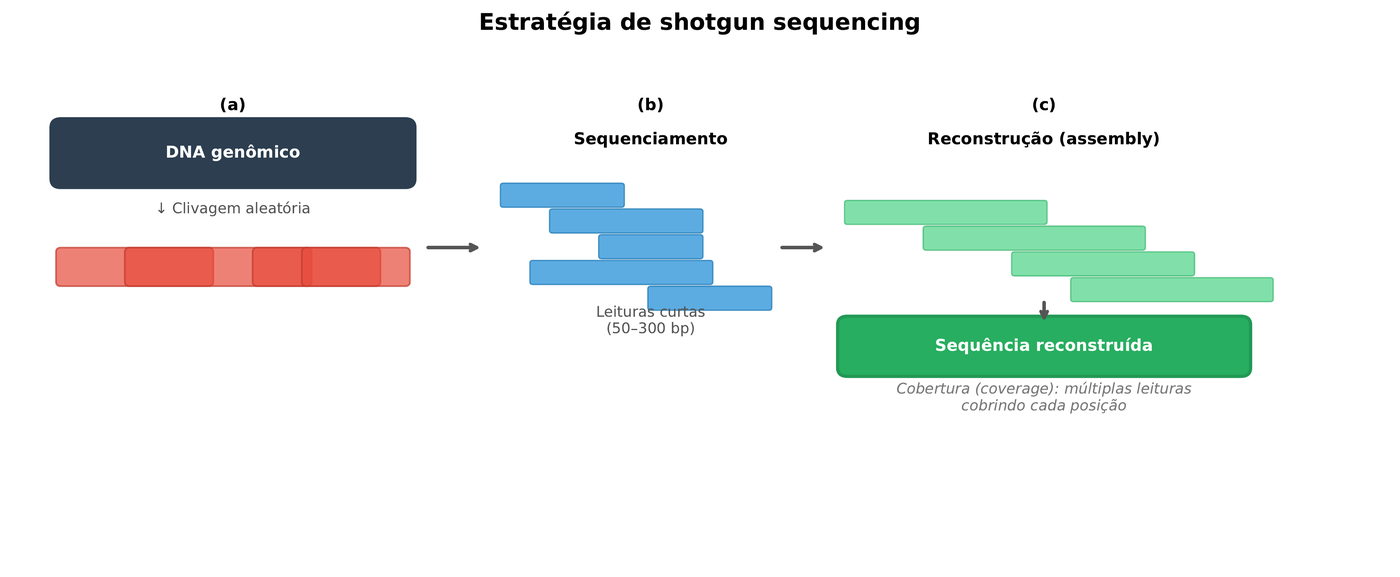
\includegraphics[width=0.85\textwidth]{imagens/shotgun_sequencing.png}
    \caption{Diagrama ilustrativo do processo de \textit{shotgun sequencing}: clivagem aleatória do DNA genômico em fragmentos, sequenciamento em leituras curtas e sobreposição para reconstrução da sequência original.}
    \label{fig:shotgun}
\end{figure}

Na montagem genômica, fragmentos sobrepostos são inicialmente agrupados em \textbf{contigs} (\textit{contiguous sequences} --- sequências contínuas reconstruídas a partir do alinhamento de leituras sobrepostas, análogas a blocos de texto já montados). Quando existe informação adicional que permite inferir a ordem relativa entre diferentes contigs --- como dados de \textbf{leituras pareadas} (\textit{paired-end reads}: pares de leituras gerados a partir das duas extremidades do mesmo fragmento de DNA, com distância conhecida entre elas) ---, esses podem ser organizados em estruturas mais amplas chamadas \textbf{scaffolds}. Assim, enquanto os contigs representam sequências consolidadas diretamente a partir das leituras, os scaffolds constituem hipóteses mais abrangentes sobre a organização genômica, servindo como passo intermediário até a obtenção de montagens completas e anotadas.

As tecnologias de NGS diferem substancialmente no comprimento das leituras produzidas. Sequenciadores Illumina, por exemplo, geram leituras curtas de alta acurácia (50 a 300 pares de bases), que exigem algoritmos sofisticados para lidar com regiões repetitivas. Em contrapartida, tecnologias como PacBio e Oxford Nanopore produzem leituras longas, que podem alcançar milhares de pares de bases em uma única sequência, favorecendo a continuidade da montagem, ainda que a custos mais elevados e com menor rendimento global \cite{ekblom2014}.

% [SUGESTÃO DE FIGURA]: Tabela comparativa das tecnologias de sequenciamento
\begin{figure}[H]
    \centering
    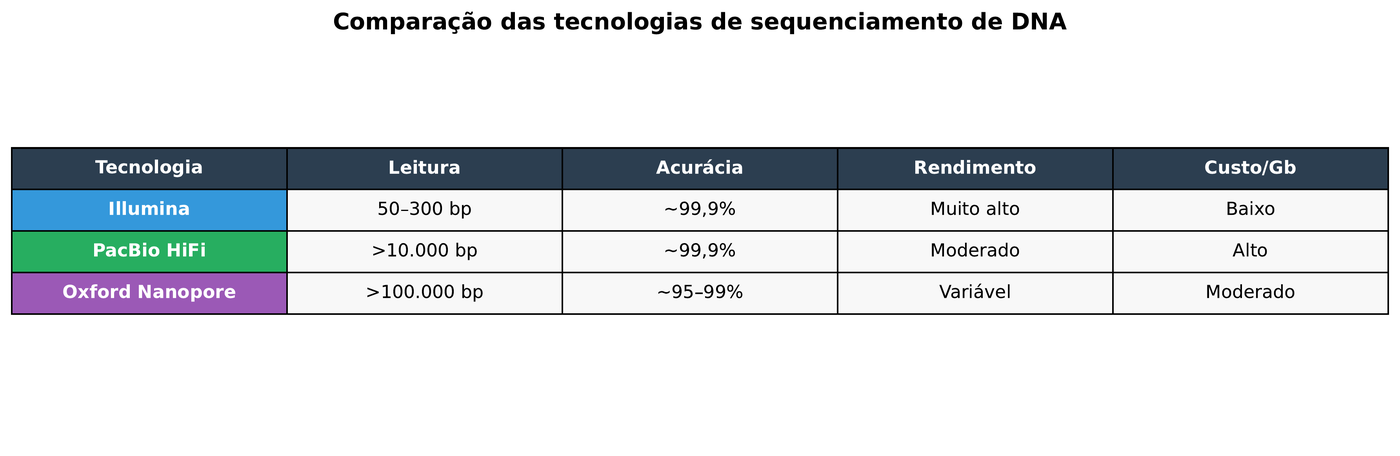
\includegraphics[width=0.85\textwidth]{imagens/tabela_tecnologias_seq.png}
    \caption{Comparativo das principais tecnologias de sequenciamento: Illumina (leituras curtas, alta acurácia), PacBio HiFi (leituras longas, alta fidelidade) e Oxford Nanopore (leituras ultra-longas, menor acurácia).}
    \label{fig:tecnologias_seq}
\end{figure}

O DNA mitocondrial (mtDNA) reúne um conjunto de particularidades que o tornam um alvo privilegiado para a montagem \textit{de novo}. Antes de descrevê-las, convém definir conceitos fundamentais da biologia molecular que serão recorrentes ao longo deste trabalho.

Um \textbf{gene} é um trecho de DNA que contém as instruções para a síntese de uma molécula funcional --- geralmente uma \textbf{proteína}, macromolécula que executa a maioria das funções celulares (catálise enzimática, transporte de substâncias, estrutura celular). O DNA é composto por uma sequência de \textbf{nucleotídeos}, unidades químicas identificadas pelas letras A (adenina), T (timina), G (guanina) e C (citosina). Dois nucleotídeos complementares em fitas opostas (A com T, G com C) formam um \textbf{par de bases} (bp, do inglês \textit{base pair}), a unidade de medida padrão para comprimento de sequências genômicas. A informação genética contida no DNA é lida em blocos de três nucleotídeos consecutivos chamados \textbf{códons}: cada códon especifica um \textbf{aminoácido}, os ``blocos de construção'' das proteínas (existem 20 aminoácidos padrão, como fenilalanina, valina, isoleucina, entre outros). Um gene que codifica uma proteína possui um \textbf{códon de início} (tipicamente ATG, que sinaliza onde a tradução deve começar) e um \textbf{códon de término} ou \textbf{códon de parada} (como TAA, TAG ou TGA, que sinaliza onde a tradução deve parar). O fluxo da informação genética segue o chamado \textbf{dogma central da biologia molecular}: o DNA é transcrito em \textbf{RNA mensageiro} (mRNA), que por sua vez é traduzido em proteína pelos \textbf{ribossomos} --- complexos macromoleculares compostos por proteínas e \textbf{RNA ribossomal} (rRNA). Nesse processo de tradução, cada códon do mRNA é reconhecido por uma molécula de \textbf{RNA transportador} (tRNA), que carrega o aminoácido correspondente e o posiciona no ribossomo para ser incorporado à cadeia proteica em crescimento. A região do tRNA que reconhece o códon é chamada \textbf{anticódon} --- uma sequência de três nucleotídeos complementar ao códon do mRNA \cite{alberts2022}.

Em metazoários (animais multicelulares), o mtDNA corresponde a uma molécula \textbf{circular} de fita dupla --- diferentemente dos \textbf{cromossomos} nucleares (estruturas lineares de DNA compactado localizadas no núcleo da célula, que carregam a maior parte da informação genética), que são lineares, o DNA mitocondrial forma um anel contínuo sem extremidades ---, com tamanho geralmente entre 12 e 22 mil pares de bases, codificando 37 genes distribuídos em 13 proteínas associadas à \textbf{fosforilação oxidativa} (o conjunto de reações bioquímicas que a mitocôndria utiliza para produzir ATP, a molécula de energia da célula), 22 tRNAs e 2 rRNAs \cite{anderson1981,asakawa1995,boore1999}. Em sua revisão seminal, \citeonline{boore1999} observou que, embora a economia extrema de tamanho seja aparente em muitos casos, essa visão --- até então quase axiomática --- é refutada por mitogenomas com grandes quantidades de sequência não codificante descobertos em alguns artrópodes, moluscos e nematódeos, demonstrando que as pressões seletivas sobre o tamanho do mtDNA variam substancialmente entre linhagens. O sequenciamento completo do genoma mitocondrial humano por \citeonline{anderson1981} representou um marco histórico, estabelecendo o modelo de referência para a organização gênica mitocondrial dos metazoários.

% [SUGESTÃO DE FIGURA]: Representação circular de um genoma mitocondrial típico
\begin{figure}[H]
    \centering
    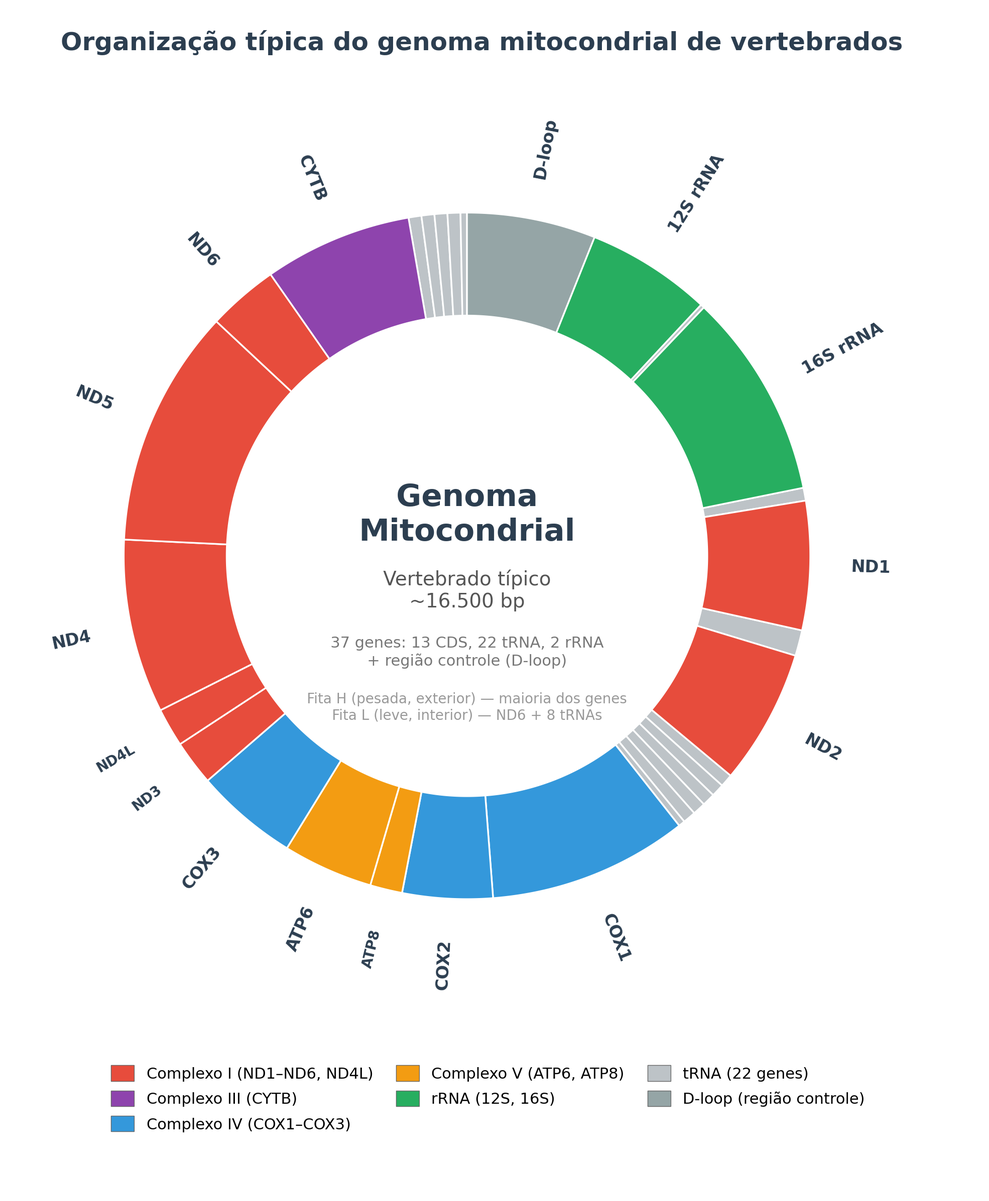
\includegraphics[width=0.75\textwidth]{imagens/mitogenoma_vertebrado_esquematico.png}
    \caption{Representação circular esquemática de um genoma mitocondrial típico de vertebrado, mostrando a distribuição dos 37 genes (13 CDS, 22 tRNAs, 2 rRNAs), a região controle (D-loop) e as fitas pesada (H) e leve (L).}
    \label{fig:mitogenoma_esquematico}
\end{figure}

A ausência de \textbf{íntrons} (segmentos não codificantes que, nos genes nucleares, intercalam as regiões codificantes e precisam ser removidos antes da tradução), a estrutura compacta e a elevada taxa de cópias por célula tornam o mtDNA especialmente acessível, facilitando sua recuperação mesmo em experimentos voltados ao genoma nuclear, nos quais ele aparece como subproduto. Além disso, características funcionais como a herança predominantemente materna, a ausência geral de recombinação e a taxa evolutiva superior à do DNA nuclear ampliam sua utilidade em estudos biológicos. Essas propriedades explicam sua ampla aplicação em análises de genética de populações, \textbf{filogeografia} (estudo da distribuição geográfica de linhagens genéticas), sistemática e conservação da biodiversidade.

Para explorar essas vantagens, foram desenvolvidos algoritmos específicos de montagem. Uma das abordagens mais empregadas é a \textit{seed-and-extend} (semente-e-extensão), em que uma sequência inicial conhecida (\textit{seed} --- semente) --- que pode ser um gene ou até mesmo um fragmento de organela de espécie próxima --- serve como ponto de partida para estender iterativamente a montagem até que a molécula circular seja reconstruída. Quando as extremidades da sequência em construção se sobrepõem, confirmando que o genoma forma um anel contínuo, diz-se que a montagem foi \textbf{circularizada} --- indicação de que o genoma mitocondrial completo foi recuperado com sucesso. O NOVOPlasty é um dos principais programas baseados nessa estratégia, destacando-se pela eficiência na recuperação de genomas mitocondriais e cloroplastidiais a partir de dados de genoma total \cite{dierckxsens2017}. Avanços recentes, como o pipeline MitoHiFi, exploram leituras longas de alta fidelidade, evidenciando a constante evolução das ferramentas voltadas à montagem de organelas \cite{ulianosilva2023}.

% [SUGESTÃO DE FIGURA]: Diagrama da estratégia seed-and-extend
\begin{figure}[H]
    \centering
    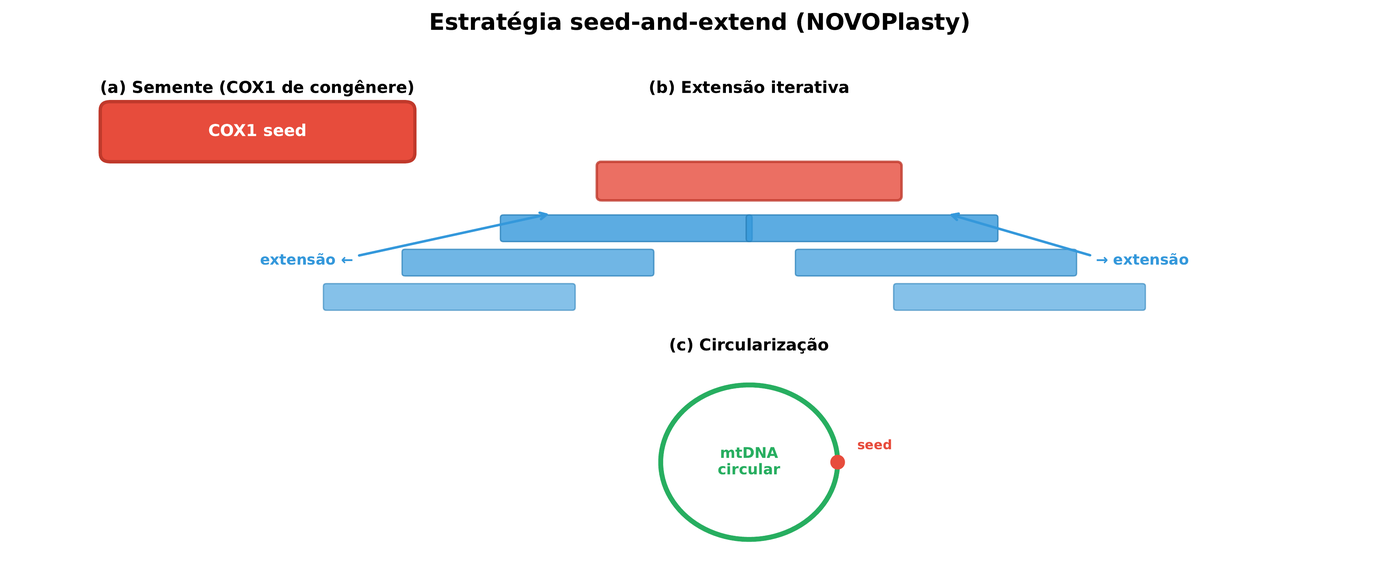
\includegraphics[width=0.85\textwidth]{imagens/seed_and_extend.png}
    \caption{Diagrama ilustrativo da estratégia \textit{seed-and-extend}: (a) sequência semente; (b) extensão iterativa a partir de leituras sobrepostas; (c) circularização quando as extremidades se encontram.}
    \label{fig:seed_extend}
\end{figure}

Complementarmente à montagem, a \textbf{anotação funcional} dos genes mitocondriais permite identificar e classificar os elementos codificantes da molécula reconstruída --- ou seja, determinar quais genes estão presentes, suas posições exatas e suas funções biológicas. Para metazoários, ferramentas como o MITOS2 combinam alinhamentos de homologia (comparações com genes conhecidos em bancos de dados) com modelos de covariância (Infernal) para predizer genes codificadores de proteínas, tRNAs e rRNAs, produzindo anotações em formatos padronizados como \textbf{GFF3} (\textit{General Feature Format version 3} --- formato tabular que especifica a localização e o tipo de cada gene no genoma) \cite{donath2019}. A integração da etapa de anotação em pipelines automatizados de montagem permanece, contudo, uma lacuna na maioria das soluções disponíveis na literatura. A ampla adoção do MITOS2 pela comunidade científica --- empregado como ferramenta primária de anotação em estudos recentes abrangendo vertebrados \cite{zhan2024,kundu2024}, invertebrados terrestres \cite{shi2024,tao2024} e invertebrados marinhos \cite{wei2024,alboasud2024} --- atesta a confiabilidade de seus resultados e reforça a pertinência de sua integração em fluxos automatizados.

\section{Reprodutibilidade em Ciência Computacional}

A reprodutibilidade é um pilar do método científico, consistindo na capacidade de um pesquisador independente replicar um experimento, com os mesmos materiais e métodos, e obter resultados consistentes. Em pesquisas computacionais, isso se traduz na possibilidade de executar o mesmo código e software sobre os mesmos dados e chegar ao mesmo resultado \cite{peng2011,sandve2013}.

Contudo, a ciência moderna enfrenta o que tem sido amplamente denominado como uma ``crise de reprodutibilidade''. Em uma pesquisa abrangente com 1.576 pesquisadores de diversas áreas, \citeonline{baker2016} revelou que 90\% dos entrevistados reconhecem a existência dessa crise --- sendo que 52\% a consideram significativa e 38\% a classificam como leve. Uma barreira crítica identificada por \citeonline{peng2011} é que, em muitos casos, o código computacional utilizado nas análises simplesmente não está mais disponível: softwares interativos frequentemente não registram as ações dos usuários de forma concreta, e mesmo quando scripts são utilizados, a combinação de múltiplos pacotes raramente é preservada de modo reprodutível. No domínio da bioinformática, essa crise é particularmente acentuada devido à alta complexidade dos pipelines de análise. Um único pipeline pode envolver dezenas de ferramentas de software distintas, cada uma desenvolvida por diferentes grupos, em diferentes linguagens de programação e com um conjunto único e, por vezes, conflitante de dependências de bibliotecas e do próprio sistema operacional. A tarefa de instalar e configurar manualmente esse ecossistema de software para replicar uma análise é extremamente suscetível a erros, uma condição frequentemente descrita como \textit{dependency hell} (inferno de dependências) \cite{gruning2018}.

Pequenas variações na versão de uma ferramenta ou de uma biblioteca subjacente podem levar a resultados drasticamente diferentes, comprometendo a validade e a confiabilidade da pesquisa. Essa barreira técnica não apenas dificulta a verificação dos resultados, mas também impede a reutilização e a adaptação de métodos computacionais, contrariando os princípios FAIR (\textit{Findable, Accessible, Interoperable, and Reusable}), que visam maximizar o valor dos dados e das análises científicas ao enfatizar, em particular, a capacidade de máquinas encontrarem e utilizarem dados automaticamente \cite{sandve2013,wilkinson2016,gruning2018,bes2017}.

% [SUGESTÃO DE FIGURA]: Diagrama comparativo do dependency hell
\begin{figure}[H]
    \centering
    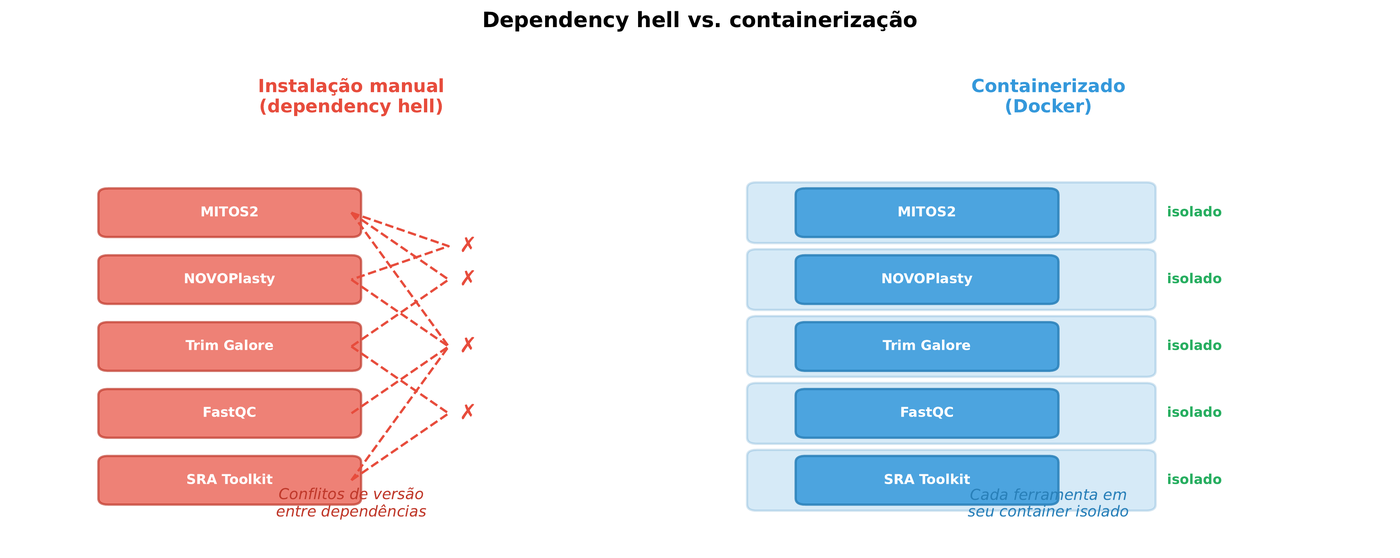
\includegraphics[width=0.85\textwidth]{imagens/dependency_hell.png}
    \caption{Diagrama comparativo do ``inferno de dependências'': à esquerda, instalação manual com conflitos entre versões; à direita, pipeline containerizado com Docker, cada ferramenta em seu container isolado.}
    \label{fig:dependency_hell}
\end{figure}

\section{Tecnologia de Conteinerização com Docker}

Como solução para o problema do \textit{dependency hell} e para garantir a reprodutibilidade computacional, a comunidade científica tem adotado práticas e tecnologias da engenharia de software, com destaque para a virtualização em nível de sistema operacional, também conhecida como containerização. A plataforma Docker se estabeleceu como a principal ferramenta desse paradigma, permitindo o empacotamento de uma aplicação e de todo o seu ambiente de execução --- incluindo bibliotecas, códigos-fonte e dependências --- em uma unidade padronizada e isolada chamada container \cite{merkel2014,gruning2018}.

O funcionamento do Docker baseia-se em dois conceitos centrais: a imagem e o container. A imagem é um template estático e imutável, construído a partir de um arquivo de texto com instruções sequenciais chamado Dockerfile. Esse arquivo serve como uma ``receita'' que define o sistema operacional base, as dependências a serem instaladas e os comandos a serem executados, criando um ambiente de software completo e autocontido. O container, por sua vez, é uma instância executável e isolada de uma imagem. Ao contrário de máquinas virtuais tradicionais, os containers compartilham o kernel do sistema operacional hospedeiro, o que os torna leves e eficientes para iniciar \cite{bes2017}.

Essa arquitetura garante que um software containerizado se comporte de maneira idêntica em qualquer ambiente que possua o Docker instalado --- seja em computadores pessoais, servidores de produção ou ambientes de nuvem --- resolvendo de forma eficaz o problema da inconsistência de ambientes e sendo um passo fundamental para a criação de pipelines científicos portáveis e reprodutíveis \cite{ditommaso2017}.

% [SUGESTÃO DE FIGURA]: Diagrama de camadas da arquitetura Docker
\begin{figure}[H]
    \centering
    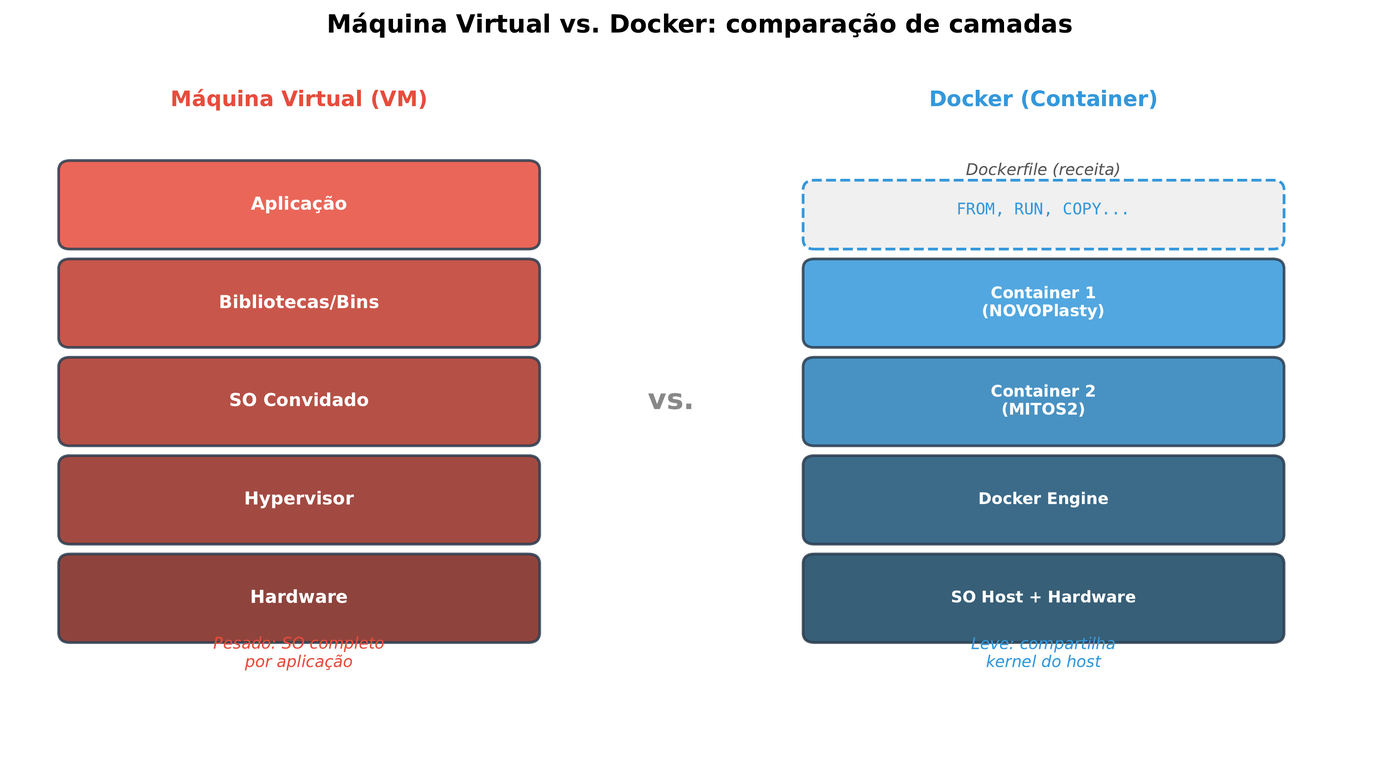
\includegraphics[width=0.85\textwidth]{imagens/docker_vs_vm.png}
    \caption{Comparação entre containers Docker e máquinas virtuais (VM): Dockerfile (receita textual), imagem (template imutável) e container (instância em execução), evidenciando a leveza dos containers.}
    \label{fig:docker_vs_vm}
\end{figure}

\section{Sistemas de Gerenciamento de Workflows Científicos}

A containerização resolve a questão do ambiente de software, mas não a orquestração das múltiplas etapas que compõem uma análise bioinformática. A execução manual e sequencial de cada container é ineficiente e propensa a erros. Para gerenciar essa complexidade, foram desenvolvidos Sistemas de Gerenciamento de Workflows (\textit{Workflow Management Systems}), como o Nextflow \cite{ditommaso2017} e o Snakemake \cite{koster2012}. Essas plataformas permitem que os pesquisadores definam pipelines computacionais complexos por meio de linguagens de alto nível.

Nesses sistemas, um workflow é decomposto em uma série de processos ou regras interconectadas. Cada processo define uma tarefa computacional discreta, especificando seus comandos, suas entradas (arquivos ou variáveis) e suas saídas. O gerenciador de workflow é então responsável por monitorar o estado dos dados e executar os processos na ordem correta, automatizando o fluxo de informação entre as etapas.

A principal vantagem dessas ferramentas reside na abstração da camada de execução. Elas integram-se nativamente com tecnologias como Docker, permitindo que cada processo seja executado em seu próprio container pré-configurado. Além disso, são compatíveis com diversos ambientes de execução, desde computadores pessoais até clusters de computação de alto desempenho (HPC) e plataformas de nuvem. Isso confere ao pipeline características essenciais para a ciência moderna: portabilidade, escalabilidade e retomada automática (\textit{resumability}) em caso de falhas, evitando o reprocessamento de etapas já concluídas.

A combinação de um gerenciador de workflows com a containerização é hoje considerada o padrão-ouro para o desenvolvimento de pipelines de bioinformática, sendo a base de iniciativas comunitárias como o nf-core, que busca padronizar e compartilhar pipelines que seguem as melhores práticas de reprodutibilidade \cite{ewels2020}.

O referencial teórico expôs os conceitos fundamentais que dão suporte à proposta deste trabalho, abordando desde os princípios de montagem \textit{de novo} de genomas até as soluções contemporâneas de reprodutibilidade, como a containerização e os sistemas de gerenciamento de workflows. Esses conceitos fornecem a base conceitual sobre a qual se apoiam os trabalhos relacionados, discutidos no Capítulo~\ref{cap:trabalhos}, que permitem situar a presente proposta no estado da arte da bioinformática aplicada à montagem de mitogenomas.

% ============================================================================
% CAPÍTULO 3 — TRABALHOS RELACIONADOS
% ============================================================================

\chapter{Trabalhos Relacionados}
\label{cap:trabalhos}

Nesta seção, são apresentados e analisados trabalhos recentes da literatura que, assim como este projeto, propõem soluções computacionais para a montagem de genomas de organelas. O objetivo desta análise comparativa é contextualizar a presente proposta no estado da arte da área, identificando as abordagens metodológicas existentes e destacando os diferenciais e a contribuição original do pipeline a ser desenvolvido neste trabalho.

\section{MitoHiFi: Montagem com Leituras Longas}

Um trabalho de destaque na área é o MitoHiFi, um pipeline desenvolvido para a montagem de genomas mitocondriais a partir de dados de \textbf{leituras longas} de alta fidelidade (PacBio HiFi --- tecnologia que produz leituras de milhares de pares de bases com alta precisão, em contraste com as leituras curtas de 100--300 bp geradas pela plataforma Illumina). Proposto por \citeonline{ulianosilva2023}, o objetivo principal era criar um método que aproveitasse a extensão e a precisão deste tipo de dado para gerar mitogenomas completos e corretamente circularizados com maior eficiência. A metodologia do MitoHiFi integra ferramentas como o \textit{hifiasm-meta} para montagem e o GetOrganelle para a etapa de finalização, sendo orquestrada por meio de scripts em Shell e utilizando \textbf{Conda} (gerenciador de pacotes e ambientes, alternativa ao Docker para gestão de dependências de software) para o gerenciamento das dependências.

A abordagem do MitoHiFi é extremamente atual por focar em uma tecnologia de sequenciamento de ponta. Seus resultados são expressivos: o pipeline foi utilizado para montar 374 mitogenomas (368 Metazoa e 6 Fungi) em projetos como o Darwin Tree of Life, o Vertebrate Genomes Project e o Aquatic Symbiosis Genome Project, além de identificar automaticamente variantes decorrentes de heteroplasmia e inserções nucleares de sequências mitocondriais (NUMTs) \cite{ulianosilva2023}. No entanto, sua implementação via scripts e Conda, embora eficaz para seu propósito, pode apresentar limitações de portabilidade e reprodutibilidade quando comparada a soluções baseadas em containers e sistemas de workflow. O diferencial do presente TCC reside precisamente neste ponto: enquanto o MitoHiFi inova na aplicação de um novo tipo de dado biológico, nossa proposta foca em uma arquitetura de software mais robusta, utilizando Docker e Nextflow, para garantir que o pipeline de montagem (baseado em leituras curtas) seja universalmente reprodutível e portável.

\section{MITObim: Estratégia de \textit{Baiting and Iterative \mbox{Mapping}}}

O MITObim, desenvolvido por \citeonline{hahn2013}, foi um dos primeiros métodos amplamente utilizados para montagem de organelas a partir de dados de NGS. Sua estratégia de \textit{baiting and iterative mapping} (captura e mapeamento iterativo) consiste em iniciar o processo com uma sequência guia (um fragmento do genoma alvo ou de uma espécie próxima) e, a partir dela, recuperar leituras homólogas (isto é, leituras suficientemente similares à sequência guia para corresponderem ao genoma mitocondrial), refinando o alinhamento de forma iterativa até a montagem completa do mitogenoma.

Em testes com dados reais de NGS, o MITObim demonstrou capacidade de recuperar mitogenomas completos com acurácia superior a 99,5\% em menos de 24 horas utilizando um computador desktop padrão \cite{hahn2013}. Apesar desses resultados e de sua relevância histórica como pioneiro na abordagem, o MITObim apresenta limitações em termos de eficiência computacional e escalabilidade, especialmente quando aplicado a conjuntos de dados maiores ou de maior complexidade, vindo a ser gradualmente substituído por ferramentas mais modernas, como o NOVOPlasty e o GetOrganelle.

\section{GetOrganelle: Montagem Baseada em Grafos}

O GetOrganelle, proposto por \citeonline{jin2020}, é uma das ferramentas mais recentes e populares para montagem de organelas. Ele utiliza \textbf{grafos de montagem} (estruturas matemáticas em que os nós representam fragmentos de sequência e as arestas representam sobreposições entre eles) derivados de dados de NGS para isolar e reconstruir genomas de organelas, oferecendo resultados robustos tanto para mitocôndrias quanto para cloroplastos (organelas fotossintetizantes de plantas). Em uma avaliação sistemática com 50 datasets publicados de plantas, o GetOrganelle foi capaz de remontar plastomas circulares em 47 dos 50 casos --- uma taxa de sucesso significativamente superior à do NOVOPlasty. Além disso, a avaliação por mapeamento de reads demonstrou que os plastomas montados pelo GetOrganelle são geralmente mais acurados que os publicados originalmente ou remontados pelo NOVOPlasty \cite{jin2020}. A ferramenta tem se destacado também por sua capacidade de gerar todas as configurações possíveis quando os genomas apresentam configurações \textit{flip-flop} ou outros isômeros mediados por repetições, oferecendo resultados consistentes mesmo em organismos com maior complexidade genômica.

No entanto, assim como outras ferramentas tradicionais, o GetOrganelle depende de um ambiente de software adequado para ser executado, geralmente configurado manualmente pelo usuário ou via gerenciadores como Conda, o que ainda pode limitar sua reprodutibilidade plena em diferentes contextos computacionais. Cabe notar que, embora o GetOrganelle apresente taxas de sucesso e acurácia superiores ao NOVOPlasty em plastomas de plantas, a literatura recente demonstra que o NOVOPlasty permanece como a ferramenta predominante para montagem de mitogenomas de metazoários --- sendo adotado em estudos recentes de larga escala com 213 mitogenomas de lagartos \cite{zhan2024} e em trabalhos individuais de peixes, arraias, moluscos e invertebrados \cite{kundu2024,guerreiro2025,shi2024,tao2024}. Essa preferência pela comunidade reforça a escolha do NOVOPlasty como montador neste pipeline.

\section{MToolBox: Foco em Genomas Mitocondriais Humanos}

O MToolBox, apresentado por \citeonline{calabrese2014}, foi uma das primeiras pipelines integradas voltadas especificamente para o estudo de genomas mitocondriais humanos. Ele combina montagem, anotação e análise funcional em um único fluxo, permitindo identificar \textbf{variantes mitocondriais} (alterações pontuais na sequência de DNA que distinguem indivíduos ou populações) relevantes para estudos biomédicos e populacionais.

Apesar de sua contribuição para o campo, o MToolBox é fortemente orientado ao contexto humano e não é tão amplamente aplicável a outros organismos. Além disso, por ter sido desenvolvido antes da adoção massiva de containers e workflows, carece de recursos de portabilidade e reprodutibilidade presentes em soluções mais modernas.

\section{MitoZ: Pipeline Integrado para Metazoários}

O MitoZ, proposto por \citeonline{meng2019}, é um toolkit que integra as etapas de montagem \textit{de novo}, anotação e visualização de genomas mitocondriais de animais em um único fluxo de trabalho. Internamente, o MitoZ utiliza o montador MEGAHIT para a montagem, o programa \texttt{cmsearch} (da suíte Infernal) para predição de tRNAs baseada em modelos de covariância, e gera automaticamente mapas circulares do mitogenoma. Em benchmarks com 50 amostras, o MitoZ demonstrou capacidade de recuperar mais mitogenomas completos e com maior acurácia que o NOVOPlasty isolado (similaridade $>$97\% com referências Sanger para a maioria dos genes) \cite{meng2019}.

Uma vantagem relevante do MitoZ é a disponibilidade de imagem Docker oficial e suporte a Singularity, além da instalação via Bioconda. No entanto, a ferramenta não utiliza um gerenciador de workflow (como Nextflow ou Snakemake), sendo executada como um pipeline monolítico em Python/Shell. Além disso, é restrita a genomas mitocondriais de \textbf{animais}, não oferecendo suporte a plastomas ou outros organismos. Os desenvolvedores recomendam limitar os dados de entrada a aproximadamente 0,3\,Gbp, pois volumes excessivos podem impedir a circularização.

\section{MitoFinder: Extração em Larga Escala}

O MitoFinder, desenvolvido por \citeonline{allio2020}, foi projetado para extração automatizada e em larga escala de dados mitogenômicos, especialmente a partir de bibliotecas de captura por enriquecimento de alvos (UCE --- \textit{Ultraconserved Elements}), embora também seja aplicável a dados de sequenciamento de genoma completo. A ferramenta oferece flexibilidade na escolha do montador (MEGAHIT, MetaSPAdes ou IDBA-UD) e realiza a anotação de genes codificadores e rRNAs via BLAST contra um genoma de referência fornecido pelo usuário, com predição de tRNAs por MiTFi, ARWEN ou tRNAscan-SE.

Em estudo com 501 bibliotecas UCE de formigas (Formicidae), o MitoFinder recuperou 296 mitogenomas em contig único \cite{allio2020}, demonstrando sua capacidade para processamento em lote. A ferramenta possui ampla generalidade taxonômica, suportando diversos códigos genéticos do NCBI, e gera arquivos em formato GenBank prontos para submissão. Contudo, o MitoFinder foi implementado em \textbf{Python 2.7} (versão já em fim de vida), o que dificulta a instalação, e disponibiliza apenas imagem Singularity (sem Docker oficial). Assim como o MitoZ, não utiliza gerenciador de workflow.

\section{NOVOPlasty: Estratégia \textit{Seed-and-Extend}}

O NOVOPlasty, descrito por \citeonline{dierckxsens2017}, é atualmente uma das ferramentas mais utilizadas para montagem de genomas mitocondriais e cloroplastidiais a partir de dados de NGS de leituras curtas. Baseado na estratégia \textit{seed-and-extend}, o programa inicia a montagem a partir de uma sequência semente fornecida pelo usuário e estende iterativamente o genoma até que a molécula circular esteja completa. Sua popularidade decorre da facilidade de uso e da capacidade de gerar montagens confiáveis mesmo a partir de dados de genoma total. A eficácia do NOVOPlasty em aplicações de larga escala foi recentemente demonstrada por \citeonline{zhan2024}, que utilizaram a ferramenta para montar 213 mitogenomas de lagartos (Squamata), combinando-a com o MITOS2 para anotação funcional --- exatamente a mesma combinação de ferramentas adotada neste trabalho.

No entanto, o NOVOPlasty, como software isolado, ainda demanda configuração manual do ambiente e execução direta pelo usuário, o que pode dificultar sua integração em fluxos mais complexos e comprometer a reprodutibilidade quando diferentes versões ou configurações são utilizadas. É justamente neste ponto que se insere o presente TCC: ao invés de propor um novo montador, o objetivo é integrar o NOVOPlasty em um ecossistema de containers e workflow (Docker + Nextflow), assegurando que seu uso seja portável, automatizado e reprodutível em diferentes ambientes de execução.

\section{Análise Comparativa}

A Tabela~\ref{tab:comparativa} sintetiza as características das ferramentas e pipelines analisados, confrontando-as com a proposta deste trabalho. A comparação considera critérios relevantes para a reprodutibilidade, portabilidade e completude do fluxo analítico.

\begin{table}[H]
\centering
\caption{Comparação entre ferramentas de montagem de organelas e o pipeline proposto.}
\label{tab:comparativa}
\footnotesize
\resizebox{\textwidth}{!}{%
\begin{tabular}{@{}lcccccccc@{}}
\toprule
\textbf{Critério} & \textbf{MitoHiFi} & \textbf{MITObim} & \textbf{GetOrganelle} & \textbf{MToolBox} & \textbf{MitoZ} & \textbf{MitoFinder} & \textbf{NOVOPlasty} & \textbf{Este trabalho} \\
\midrule
Tipo de dado & Long reads & Short reads & Short/Long & Short reads & Short reads & Short reads & Short reads & Short reads \\
 & (HiFi) & & reads & & & & & \\
\addlinespace
Montagem & \checkmark & \checkmark & \checkmark & \checkmark & \checkmark & \checkmark & \checkmark & \checkmark \\
\addlinespace
Anotação funcional & --- & --- & --- & \checkmark & \checkmark & \checkmark & --- & \checkmark \\
 & & & & (humano) & (animais) & (referência) & & (metazoários) \\
\addlinespace
Visualização & --- & --- & --- & --- & \checkmark & --- & --- & \checkmark \\
(mapa circular) & & & & & & & & (Biopython) \\
\addlinespace
GenBank Flat File & --- & --- & --- & --- & --- & \checkmark & --- & \checkmark \\
\addlinespace
Containerização & Parcial & --- & Conda & --- & Docker/ & Singularity & --- & Docker \\
 & (Conda) & & & & Singularity & & & (5 imagens) \\
\addlinespace
Workflow manager & --- & --- & --- & --- & --- & --- & --- & Nextflow DSL2 \\
\addlinespace
Pilot QC automático & --- & --- & --- & --- & --- & --- & --- & \checkmark \\
\addlinespace
Estrutura secundária & --- & --- & --- & --- & --- & --- & --- & \checkmark \\
RNA & & & & & & & & (ViennaRNA) \\
\addlinespace
Execução em laptop & Requer & Servidor & Servidor & Desktop/ & Desktop & Desktop & Desktop & \checkmark \\
 & cluster/HPC & recomendado & recomendado & servidor & & & & (notebook 16 GB) \\
\addlinespace
Código aberto & \checkmark & \checkmark & \checkmark & \checkmark & \checkmark & \checkmark & \checkmark & \checkmark \\
\bottomrule
\end{tabular}}%
\end{table}

A análise comparativa evidencia que, embora cada ferramenta contribua com inovações relevantes para domínios específicos, nenhuma oferece um fluxo integrado que cubra todas as etapas --- desde a aquisição dos dados brutos até a geração de arquivos prontos para submissão ao GenBank --- em um ambiente completamente containerizado e orquestrado. Adicionalmente, nenhuma das soluções analisadas incorpora mecanismos de redução automática do volume de dados (como o Pilot QC e o truncamento adaptativo), o que as torna dependentes de hardware com grande capacidade de armazenamento e memória. A proposta deste trabalho preenche essas lacunas ao combinar montagem, anotação funcional, geração de entregáveis, práticas de reprodutibilidade e acessibilidade computacional em um único pipeline modular, executável em computadores pessoais.

% [SUGESTÃO DE FIGURA]: Gráfico radar comparando as ferramentas

Para complementar a análise tabular, a Figura~\ref{fig:radar_comparativo} apresenta uma visualização em gráfico radar que sintetiza o desempenho relativo de cada ferramenta em cinco eixos qualitativos, pontuados em escala de 1 a 5 conforme os critérios da Tabela~\ref{tab:scores_radar}. Essa pontuação foi atribuída com base nas informações publicadas nos artigos originais de cada ferramenta e na análise direta da documentação e dos repositórios oficiais.

\begin{table}[H]
\centering
\caption{Critérios de pontuação do gráfico radar comparativo (escala 1--5).}
\label{tab:scores_radar}
\footnotesize
\resizebox{\textwidth}{!}{%
\begin{tabular}{@{}lp{10cm}@{}}
\toprule
\textbf{Eixo} & \textbf{Critério de pontuação} \\
\midrule
Reprodutibilidade & Nível de isolamento do ambiente: 1 = instalação manual; 2 = Conda; 3 = Conda + versões pinadas; 4 = Docker ou Singularity; 5 = Docker + workflow manager com versões pinadas \\
\addlinespace
Completude do fluxo & Número de etapas cobertas: 1 = apenas montagem; 2 = montagem + anotação parcial; 3 = montagem + anotação completa; 4 = inclui visualização ou conversão de formatos; 5 = fluxo completo (aquisição → montagem → anotação → entregáveis GenBank) \\
\addlinespace
Acessibilidade computacional & Requisitos de hardware: 1 = requer cluster/HPC; 2 = servidor dedicado recomendado; 3 = desktop padrão; 4 = desktop com dados reduzidos manualmente; 5 = notebook com redução automática de dados \\
\addlinespace
Automação & Grau de intervenção do usuário: 1 = configuração manual extensiva; 2 = scripts isolados; 3 = pipeline com parâmetros manuais; 4 = pipeline com defaults razoáveis; 5 = execução com um único comando + decisões automáticas (Pilot QC, fallback k-mer) \\
\addlinespace
Generalidade taxonômica & Escopo de organismos: 1 = uma espécie (e.g., humano); 2 = um grupo taxonômico restrito; 3 = metazoários; 4 = metazoários + outros eucariotos; 5 = qualquer organismo com genoma mitocondrial \\
\bottomrule
\end{tabular}}%
\end{table}

\begin{figure}[H]
    \centering
    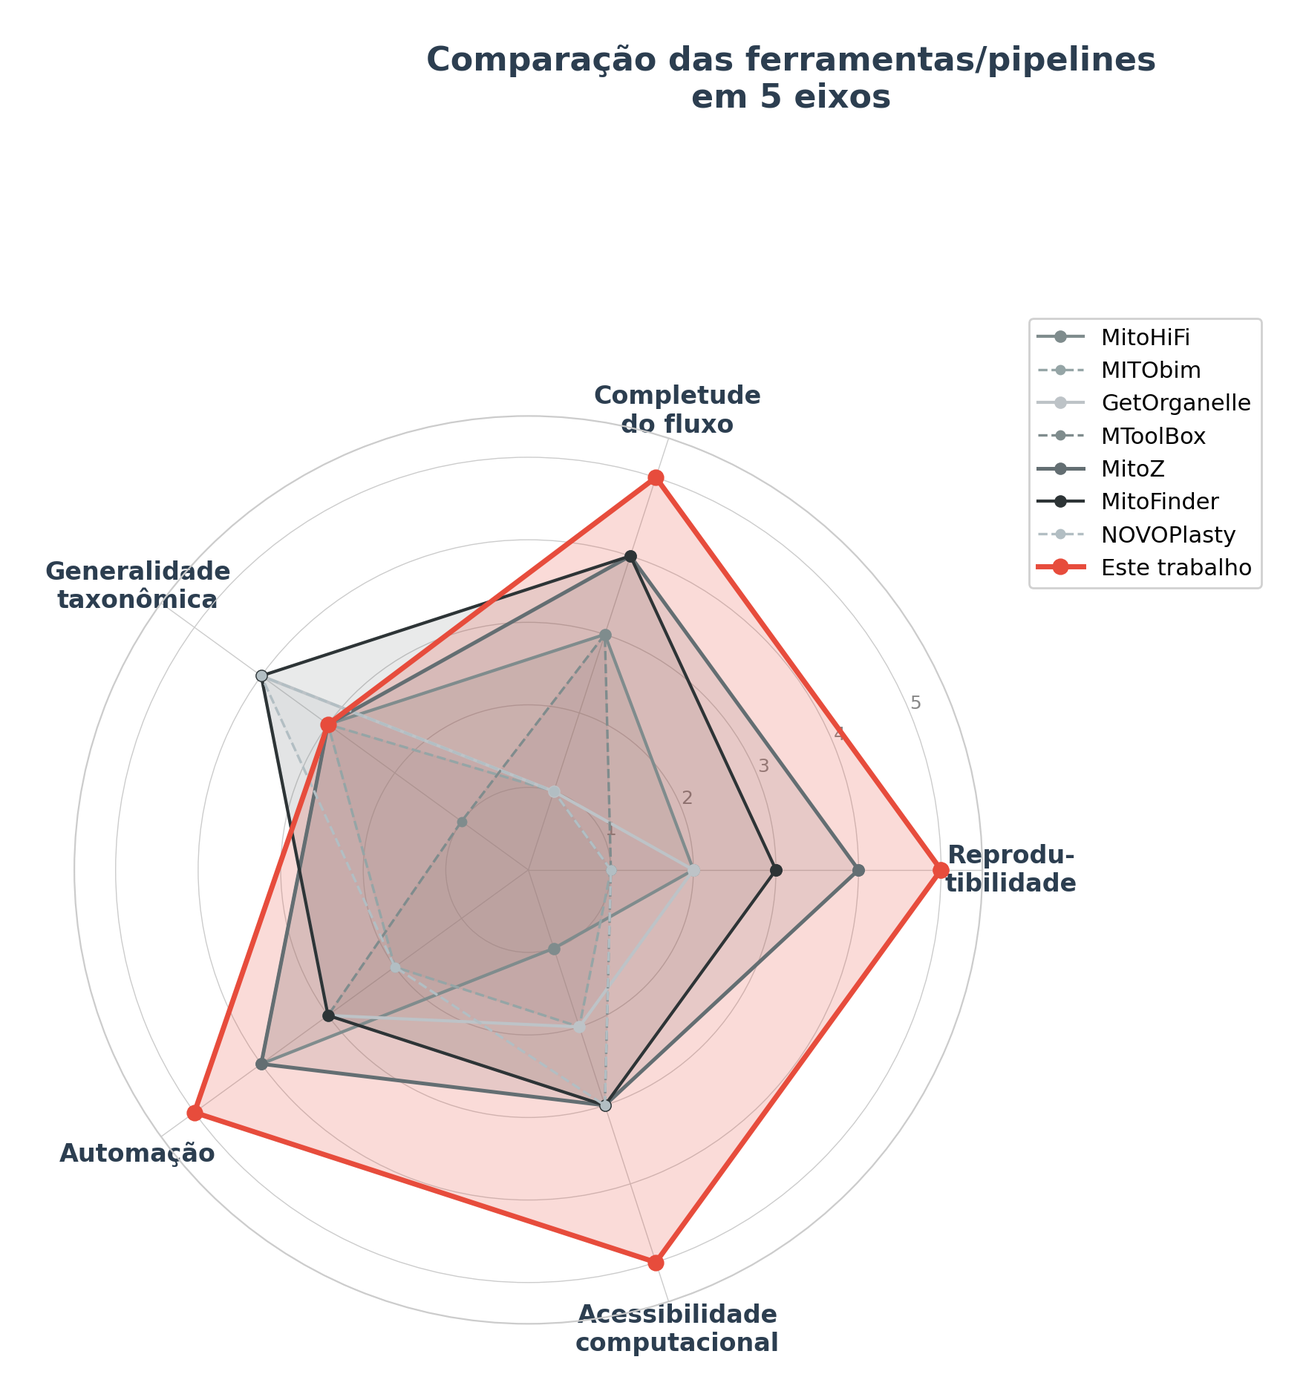
\includegraphics[width=0.80\textwidth]{imagens/radar_comparativo.png}
    \caption{Gráfico radar comparando as ferramentas analisadas em cinco eixos: completude do fluxo, reprodutibilidade, acessibilidade computacional, automação e generalidade taxonômica. A pontuação de cada eixo segue os critérios da Tabela~\ref{tab:scores_radar}.}
    \label{fig:radar_comparativo}
\end{figure}

A análise dos trabalhos relacionados permitiu identificar diferentes abordagens para a montagem de organelas, incluindo pipelines baseados em leituras longas, estratégias iterativas e montadores especializados como o NOVOPlasty. Embora cada solução apresente contribuições relevantes, permanecem lacunas quanto à padronização, portabilidade, completude do fluxo analítico e reprodutibilidade. Nesse contexto, o Capítulo~\ref{cap:metodologia} descreve a metodologia adotada neste trabalho, detalhando a concepção do pipeline proposto e as ferramentas que o compõem.

% ============================================================================
% CAPÍTULO 4 — METODOLOGIA
% ============================================================================

\chapter{Metodologia}
\label{cap:metodologia}

Nesta seção, é apresentado o plano metodológico para o desenvolvimento do pipeline de montagem de mitogenomas. A abordagem combina etapas de análise bioinformática com práticas consolidadas de engenharia de software, seguindo um processo de desenvolvimento sistemático descrito na seção 4.1, antes de detalhar a arquitetura do pipeline e suas etapas constituintes.

\section{Processo de Desenvolvimento de Software}

O desenvolvimento do pipeline seguiu uma abordagem de \textbf{desenvolvimento iterativo e incremental}, metodologia consolidada na engenharia de software em que o sistema é construído em ciclos sucessivos, cada um produzindo uma versão funcional e testável do produto \cite{larman2003}. Essa abordagem se contrapõe ao modelo cascata (\textit{waterfall}), no qual todas as fases --- levantamento de requisitos, projeto, implementação e teste --- são executadas sequencialmente e o produto só é validado ao final. No contexto de software científico, em que os requisitos frequentemente evoluem à medida que os resultados são analisados, o modelo iterativo é amplamente recomendado \cite{wilson2014}.

O ciclo de desenvolvimento foi organizado em duas fases principais, cada uma constituindo uma iteração completa com entrega funcional:

\begin{itemize}
    \item \textbf{Fase 1 --- Montagem}: implementação dos módulos de download (SRA-Toolkit), controle de qualidade (FastQC, Trim Galore) e montagem (NOVOPlasty), com containerização em Docker e orquestração via Nextflow. Ao final desta fase, o pipeline já era capaz de produzir mitogenomas completos e circularizados a partir de um acesso SRA.
    \item \textbf{Fase 2 --- Anotação e entregáveis}: adição dos módulos de análise piloto de qualidade (Pilot QC), anotação funcional (MITOS2), geração de estruturas secundárias de RNA (ViennaRNA/RNAplot), produção de arquivos para submissão ao GenBank (GenBank Flat File) e compilação automática de entregáveis.
\end{itemize}

Cada fase produziu um pipeline funcional e independente. A Fase 1 foi preservada como branch separada no repositório Git (\texttt{fase1-montagem}), permitindo uso e validação independente por terceiros --- uma prática de versionamento semântico que garante rastreabilidade e facilita a manutenção \cite{sommerville2016}.

\begin{figure}[H]
    \centering
    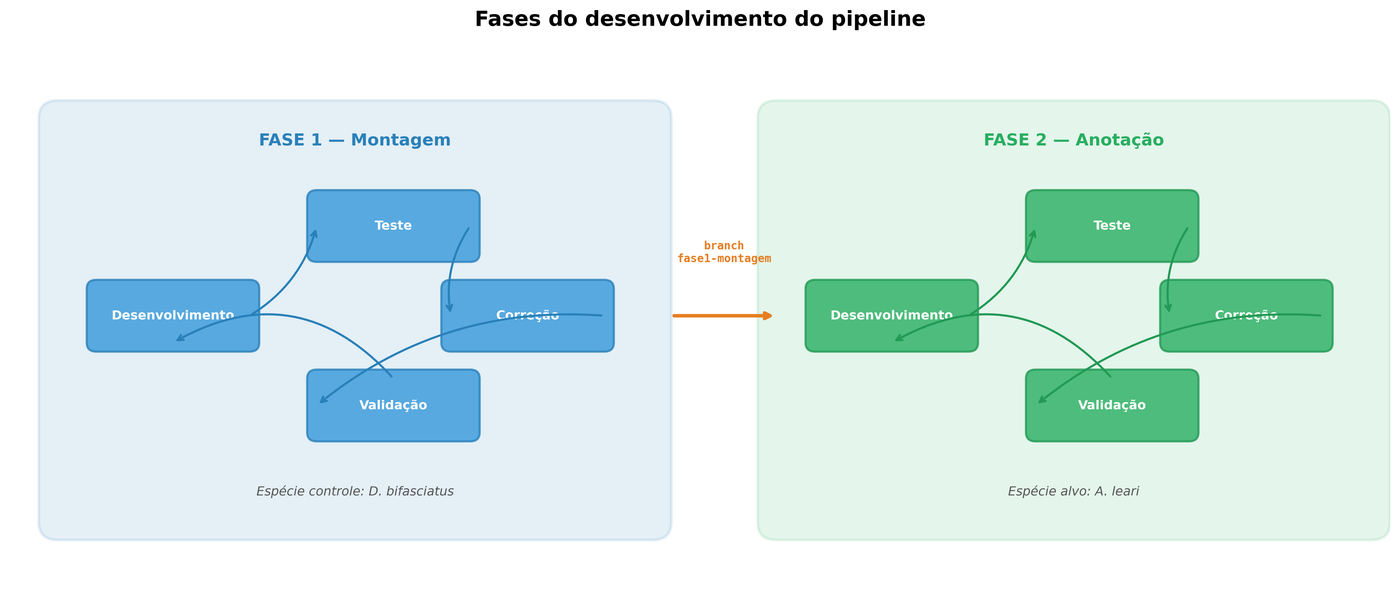
\includegraphics[width=0.85\textwidth]{imagens/fases_desenvolvimento.png}
    \caption{Diagrama de fases do desenvolvimento do pipeline: Fase 1 (Montagem) e Fase 2 (Anotação), com indicação dos ciclos iterativos e das espécies utilizadas em cada fase.}
    \label{fig:fases_desenvolvimento}
\end{figure}

\subsection{Validação por Espécie-Controle}

Um elemento central da estratégia de verificação e validação (V\&V) foi o emprego de uma \textbf{espécie-controle} com mitogenoma previamente depositado em banco de dados público. Antes de aplicar o pipeline à espécie-alvo (a arara-azul-de-lear), cuja sequência mitocondrial era inédita, o sistema foi integralmente validado com \textit{Diploprion bifasciatus}, cujo mitogenoma de referência (PZ143763.1) está depositado no GenBank. Essa estratégia permitiu comparar a montagem obtida pelo pipeline com a sequência de referência conhecida, verificando a correção funcional do sistema em condições controladas antes de aplicá-lo a dados sem referência prévia.

No desenvolvimento de software científico, a validação com dados de referência conhecida é considerada uma das práticas mais importantes para garantir a confiabilidade dos resultados computacionais \cite{wilson2014}. Essa abordagem é análoga ao conceito de \textit{oracle testing} na engenharia de software, em que uma fonte externa de verdade é utilizada para validar as saídas do sistema sob teste \cite{sommerville2016}.

\subsection{Tratamento de Erros e Correções Iterativas}

O modelo iterativo também se manifestou na resolução de problemas técnicos encontrados durante a execução do pipeline. Exemplos concretos incluem:

\begin{enumerate}
    \item \textbf{Incompatibilidade do SRA-Toolkit}: a descoberta de que o \texttt{fasterq-dump} do SRA-Toolkit 3.x não implementa o flag \texttt{-X} para limitação de leituras na origem, corrigida pela adoção de truncamento pós-conversão utilizando o utilitário \texttt{head};
    \item \textbf{Flag do RNAplot}: a incompatibilidade do flag \texttt{-{}-output-format=svg} na versão empacotada do ViennaRNA, corrigida para a sintaxe \texttt{-f svg} aceita pela versão instalada;
    \item \textbf{Frameshift do gene ND3}: a detecção, durante a análise dos resultados do MITOS2, de que o gene ND3 apresenta um frameshift biologicamente real e documentado em aves \cite{mindell1998}, levando à implementação de uma lógica de unificação (\texttt{join}) nos scripts de conversão para GenBank.
\end{enumerate}

Cada correção foi implementada, testada e integrada antes do avanço para a próxima etapa, em conformidade com o princípio de retroalimentação rápida (\textit{fail fast, fix immediately}) característico de metodologias ágeis \cite{sommerville2016}.

\subsection{Aderência às Boas Práticas de Computação Científica}

A adoção das práticas descritas acima situa este trabalho no contexto das boas práticas para computação científica sistematizadas por \citeonline{wilson2014}, que recomendam:

\begin{enumerate}
    \item \textbf{Controle de versão} para todo código-fonte --- implementado via Git com histórico completo de commits descritivos e branches para marcos significativos;
    \item \textbf{Automação de tarefas repetitivas} --- implementada via Nextflow, que orquestra todas as etapas sem intervenção manual;
    \item \textbf{Testes com dados conhecidos} --- implementados pela validação com espécie-controle (\textit{D.~bifasciatus});
    \item \textbf{Registro de dependências e ambientes} --- implementado via Dockerfiles com versões explicitamente fixadas para todas as ferramentas;
    \item \textbf{Documentação do propósito e das decisões de design} --- implementada no repositório (README, guia de execução) e neste documento.
\end{enumerate}

Essa abordagem metodológica não é apenas uma decisão de conveniência, mas uma necessidade reconhecida na literatura: estudos demonstram que a falta de práticas formais de engenharia de software em projetos científicos é uma das principais causas de irreprodutibilidade computacional \cite{baker2016,peng2011}.

\section{Visão Geral do Pipeline}

O pipeline proposto neste trabalho foi concebido para realizar a montagem e anotação de genomas mitocondriais a partir de dados de sequenciamento de nova geração (NGS), integrando ferramentas bioinformáticas consolidadas em um ambiente de execução automatizado, reprodutível e portável. A arquitetura segue uma estrutura modular, em que cada etapa corresponde a uma fase distinta do processamento dos dados, sendo encapsulada em containers Docker para garantir consistência na execução \cite{merkel2014} e integrada por meio do gerenciador de workflows Nextflow \cite{ditommaso2017}.

De forma geral, o pipeline é composto por sete macroetapas principais, organizadas em uma cadeia de redução progressiva de dados que transforma dezenas de gigabytes de leituras brutas em um mitogenoma anotado de $\sim$17~KB --- viabilizando a execução em computadores pessoais sem necessidade de servidores. A primeira é a \textbf{análise piloto de qualidade (Pilot QC)}, um estágio opcional que analisa automaticamente uma subamostra dos dados para determinar o volume ideal de leituras a serem processadas, evitando downloads desnecessários em datasets grandes. A segunda etapa é a \textbf{aquisição e preparo dos dados}, responsável por obter datasets públicos em repositórios como o Sequence Read Archive (SRA) do NCBI \cite{leinonen2011}. Em seguida, realiza-se o \textbf{controle de qualidade e pré-processamento}, que envolve a avaliação das leituras por meio do FastQC \cite{andrews2010} e a remoção de adaptadores e bases de baixa qualidade utilizando o Trim Galore \cite{babraham2019}, que por sua vez utiliza o Cutadapt \cite{martin2011} internamente.

A quarta etapa corresponde à \textbf{montagem do mitogenoma}, realizada com o NOVOPlasty, ferramenta especializada que utiliza a estratégia seed-and-extend para reconstruir a molécula circular completa a partir de leituras curtas \cite{dierckxsens2017}. A quinta etapa, de \textbf{anotação funcional}, identifica os genes do genoma montado, utilizando o MITOS2 \cite{donath2019} para a predição de genes codificadores de proteínas, rRNAs e tRNAs, com geração de estruturas secundárias previstas via ViennaRNA \cite{lorenz2011}. A sexta etapa consiste na \textbf{compilação dos entregáveis}, em que um script automatizado reúne todos os produtos da análise em uma pasta organizada, incluindo arquivos no formato GenBank Flat File para submissão ao NCBI. Por fim, a sétima etapa concentra-se na \textbf{automação e reprodutibilidade}, em que cada componente do pipeline é containerizado com Docker \cite{merkel2014} e orquestrado via Nextflow \cite{ditommaso2017}.

\begin{figure}[H]
    \centering
    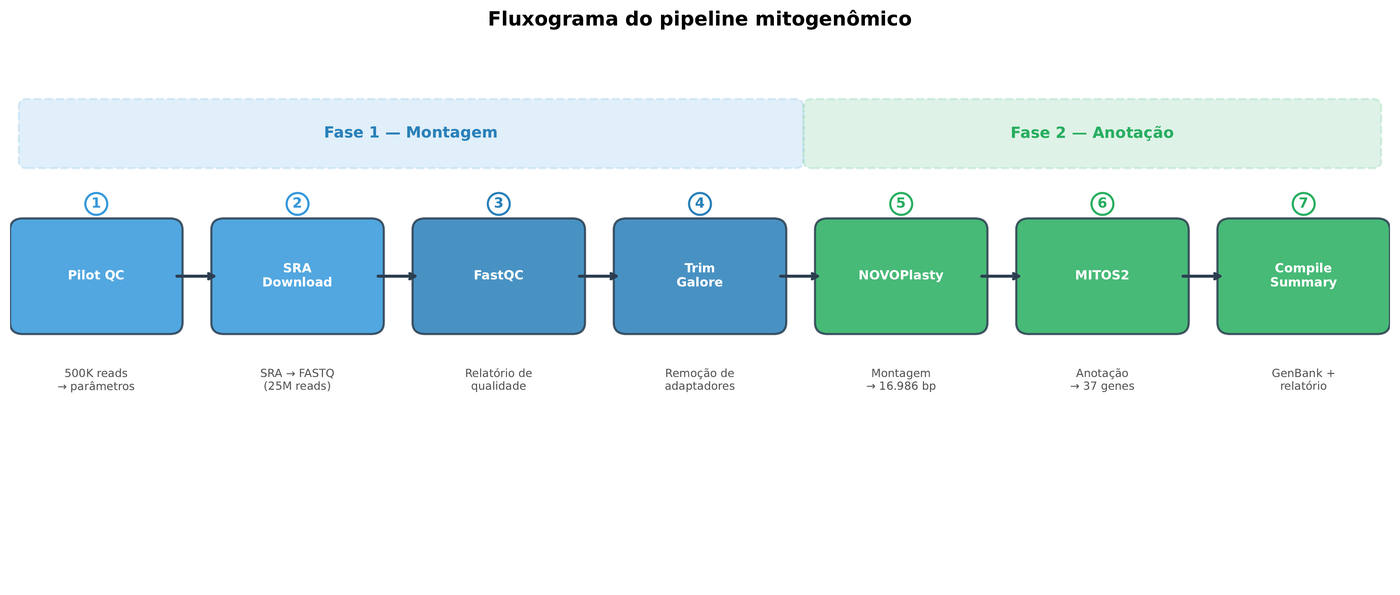
\includegraphics[width=\textwidth]{imagens/fluxograma_pipeline.png}
    \caption{Fluxograma do pipeline com as 7 etapas: Pilot QC, SRA Download, FastQC, Trim Galore, NOVOPlasty, MITOS2 e Compile Summary. Cores distinguem Fase 1 (montagem, azul) e Fase 2 (anotação, verde).}
    \label{fig:fluxograma_pipeline}
\end{figure}

A visão geral do pipeline, representada em formato de fluxograma, ilustra o encadeamento das etapas e destacando a integração entre análise bioinformática e práticas de engenharia de software. Deve-se observar que a lógica condicional do pipeline permite que a etapa de anotação (MITOS2) seja executada apenas quando o banco de dados de referência estiver disponível, tornando a Fase 1 (montagem) independente da Fase 2 (anotação). Adicionalmente, o workflow aplica um \textbf{filtro de circularização}: apenas montagens cujo nome de arquivo inicia com \texttt{Circularized\_assembly} são encaminhadas ao MITOS2 e à compilação de entregáveis. Quando o NOVOPlasty não obtém circularização (produzindo apenas contigs parciais), a anotação é automaticamente omitida, evitando análises sobre montagens incompletas que poderiam gerar resultados biologicamente incorretos. Essa decisão de design garante que os entregáveis finais representem exclusivamente genomas mitocondriais completos e circulares.

\section{Fluxo de Execução do Pipeline}

Esta seção descreve o fluxo completo de execução do pipeline, desde os pré-requisitos até a obtenção dos resultados finais, detalhando as decisões automáticas tomadas pelo sistema e o caminho percorrido pelos dados em cada~etapa.

\subsection{Pré-requisitos e Preparação do Ambiente}

Antes da primeira execução, três preparações são necessárias:

\begin{enumerate}
    \item \textbf{Construção das imagens Docker} --- o repositório inclui cinco Dockerfiles (SRA-Toolkit, FastQC, Trim Galore, NOVOPlasty e MITOS2), cada um com versões pinadas de todas as dependências. A construção é realizada por um script automatizado (\texttt{build\_images.ps1} / equivalente Bash), que gera as imagens localmente sem necessidade de registro externo;
    \item \textbf{Download do banco de dados MITOS2} --- o banco RefSeq89m ($\sim$20~MB compactado) é obtido do Zenodo e extraído em \texttt{data/databases/}. Esse passo é necessário apenas uma vez, pois o banco é reutilizado entre execuções;
    \item \textbf{Configuração do perfil da espécie} --- cada espécie requer um arquivo de configuração em \texttt{conf/} definindo o acesso SRA (\texttt{sra\_accession}), a semente (\texttt{seed}), o intervalo de tamanho esperado (\texttt{genome\_range}), os k-mers a serem tentados (\texttt{novoplasty\_\allowbreak kmers}), o código genético (\texttt{genetic\_code}) e o nome científico (\texttt{organism}).
\end{enumerate}

\subsection{Comando de Execução e Resiliência}

A execução é iniciada por um único comando:

\begin{lstlisting}
nextflow run main.nf -profile <especie>
\end{lstlisting}

Onde \texttt{<espécie>} corresponde ao nome do perfil definido em \texttt{nextflow.config} (e.g., \texttt{a\_leari}, \texttt{test}). Para execuções de longa duração --- típicas em bioinformática, onde o download de dados do SRA pode levar dezenas de minutos e a conversão dos FASTQs pode exceder uma hora ---, o pipeline inclui um script wrapper (\texttt{run\_pipeline.sh}) que encapsula a execução com \texttt{nohup}, permitindo que o terminal seja fechado ou a conexão SSH seja interrompida sem afetar o pipeline. Os logs são automaticamente direcionados para \texttt{logs/<perfil>\_<timestamp>.log}, possibilitando acompanhamento assíncrono via \texttt{tail~-f}.

Para retomar uma execução interrompida, o Nextflow oferece o mecanismo \texttt{-resume}, que reutiliza os resultados de etapas já concluídas armazenados no diretório \texttt{work/}. O pipeline organiza esse diretório por espécie e timestamp (\texttt{work/<espécie>/\allowbreak<timestamp>/}), permitindo identificar e gerenciar execuções individuais. Para retomar uma execução específica, basta indicar o diretório correspondente:

\begin{lstlisting}
nextflow run main.nf -profile <especie> -resume -w work/<especie>/<timestamp>
\end{lstlisting}

\subsection{Fluxo de Dados e Decisões Automáticas}

\begin{figure}[H]
    \centering
    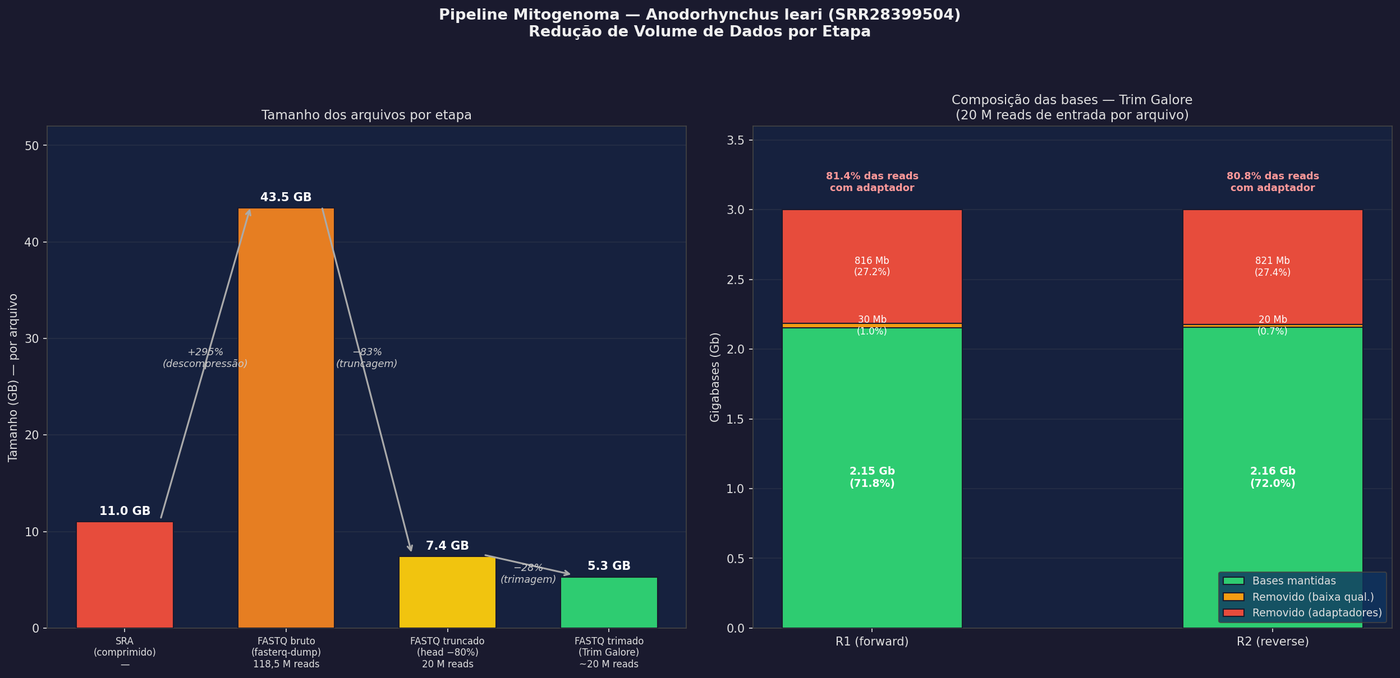
\includegraphics[width=\textwidth]{imagens/reducao_dados_pipeline.png}
    \caption{Fluxo sequencial de dados no pipeline, mostrando os formatos e volumes em cada transição, desde o arquivo \texttt{.sra} (11~GB) até os 14 entregáveis finais (1,6~MB). Destacam-se a redução de 87~GB para 17~KB e os dois pontos de decisão automática.}
    \label{fig:fluxo_dados}
\end{figure}

O pipeline incorpora dois pontos de decisão automática que não requerem intervenção do usuário:

\textbf{Decisão 1 --- Pilot QC (volume de dados).} Quando o parâmetro \texttt{sra\_max\_\allowbreak reads} não é definido no perfil da espécie, o pipeline ativa automaticamente o módulo Pilot QC (seção~\ref{sec:pilotqc}), que baixa uma subamostra de 500.000 leituras, analisa sua qualidade e calcula o número ideal de leituras para a execução principal. Quando o parâmetro é explicitamente definido (e.g., via \texttt{-{}-sra\_max\_\allowbreak reads\allowbreak{} 20000000}), o Pilot QC é pulado e o valor fornecido é utilizado diretamente. Essa lógica condicional é implementada no workflow principal (\texttt{main.nf}) por meio de operadores Nextflow de branching.

\textbf{Decisão 2 --- Filtro de Circularização (qualidade da montagem).} Após a montagem pelo NOVOPlasty, apenas arquivos cujo nome corresponde ao padrão \texttt{Circularized\_\allowbreak assembly\_*} são encaminhados ao MITOS2. Montagens parciais (contigs não circularizados) são automaticamente descartados do fluxo de anotação, evitando que genomas incompletos recebam anotações potencialmente incorretas (e.g., genes truncados nas extremidades de contigs lineares). O pipeline reporta essas montagens parciais no log para que o pesquisador possa investigar manualmente a causa da não-circularização (cobertura insuficiente, semente inadequada, ou regiões repetitivas complexas).

\begin{figure}[H]
    \centering
    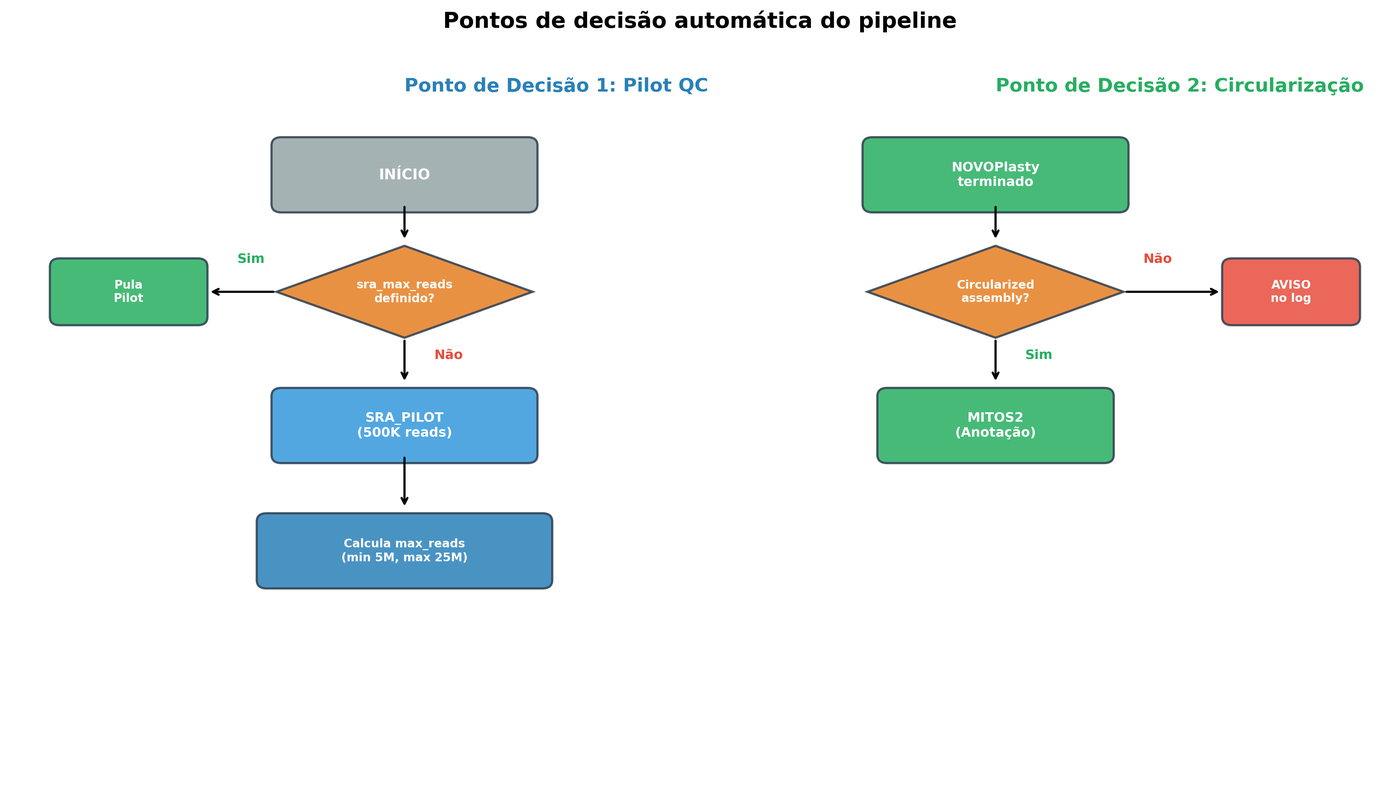
\includegraphics[width=0.85\textwidth]{imagens/diagrama_decisao.png}
    \caption{Diagrama de atividade mostrando os dois pontos de decisão automática do pipeline: (1) Pilot QC --- determina o volume de dados; (2) Filtro de Circularização --- condiciona a anotação à obtenção de genoma circularizado.}
    \label{fig:diagrama_decisao}
\end{figure}

\subsection{Extensibilidade para Novas Espécies}

A adição de uma nova espécie ao pipeline requer apenas a criação de um arquivo de configuração e a obtenção da semente correspondente, sem modificação de código-fonte. Os passos são:

\begin{enumerate}
    \item Identificar no NCBI SRA um dataset de sequenciamento de genoma total para a espécie-alvo;
    \item Localizar o mitogenoma de uma espécie \textbf{congênere} --- isto é, pertencente ao mesmo gênero taxonômico --- (ou filogeneticamente próxima) no NCBI e extrair o gene cox1 como semente;
    \item Criar um arquivo \texttt{conf/<especie>.config} definindo os parâmetros específicos (acesso SRA, semente, genome\_range, k-mers, código genético e nome);
    \item Registrar o novo perfil em \texttt{nextflow.config};
    \item Executar: \texttt{nextflow run main.nf -profile <especie>}.
\end{enumerate}

Essa arquitetura extensível é demonstrada pelas sete sementes incluídas no repositório (\texttt{data/seeds/}), que cobrem espécies de aves, peixes, insetos e nematóides, atestando a generalidade do pipeline para diferentes grupos taxonômicos.

\section{Arquitetura Modular e Scripts do Pipeline}

A organização do código segue a convenção de projetos Nextflow DSL2, em que cada etapa do pipeline corresponde a um \textbf{módulo} independente (arquivo \texttt{.nf} no diretório \texttt{modules/}), e os scripts auxiliares residem no diretório \texttt{scripts/}. Essa separação permite que cada componente seja desenvolvido, testado e mantido de forma isolada. A Tabela~\ref{tab:modulos} apresenta a relação completa dos módulos, scripts e suas responsabilidades.

\begin{longtable}{@{}p{4.5cm}p{2cm}p{7.5cm}@{}}
\caption{Arquitetura modular do pipeline: módulos, scripts e suas responsabilidades.}
\label{tab:modulos} \\
\toprule
\textbf{Arquivo} & \textbf{Tipo} & \textbf{Função} \\
\midrule
\endfirsthead
\caption[]{Arquitetura modular do pipeline (continuação).} \\
\toprule
\textbf{Arquivo} & \textbf{Tipo} & \textbf{Função} \\
\midrule
\endhead
\bottomrule
\endfoot
\texttt{main.nf} & Workflow & Orquestração geral: define a ordem de execução, lógica condicional (Pilot QC, MITOS2) e passagem de dados entre módulos \\
\addlinespace
\texttt{modules/\allowbreak sra\_download.nf} & Módulo & Download do SRA via \texttt{prefetch} + \texttt{fasterq-dump}, com truncamento por \texttt{head} \\
\addlinespace
\texttt{modules/\allowbreak fastqc.nf} & Módulo & Controle de qualidade das leituras brutas via FastQC \\
\addlinespace
\texttt{modules/\allowbreak trim\_galore.nf} & Módulo & Remoção de adaptadores e trimming de qualidade via Trim Galore \\
\addlinespace
\texttt{modules/\allowbreak novoplasty.nf} & Módulo & Montagem iterativa com múltiplos k-mers e re-seeding automático \\
\addlinespace
\texttt{modules/mitos2.nf} & Módulo & Anotação funcional via MITOS2 + geração de SVGs com RNAplot \\
\addlinespace
\texttt{scripts/pilot\_qc.sh} & Script Bash & Análise piloto: calcula Q30\%, taxa de adaptador, fração mitocondrial e recomenda \texttt{max\_reads} \\
\addlinespace
\texttt{scripts/\allowbreak compile\_summary.py} & Script Python & Compila 14 categorias de entregáveis a partir das saídas dos módulos \\
\addlinespace
\texttt{scripts/\allowbreak gff2genbank.py} & Script Python & Converte GFF3 $\rightarrow$ feature table (\texttt{.tbl}) + FASTA formatado (\texttt{.fsa}) para GenBank, com tratamento do frameshift ND3 \\
\addlinespace
\texttt{scripts/\allowbreak generate\_genbank.py} & Script Python & Gera GenBank Flat File (\texttt{.gbk}) e mapa circular (SVG/PDF) via Biopython \\
\addlinespace
\texttt{nextflow.config} & Config. & Parâmetros globais, perfis por espécie, configuração de containers Docker \\
\addlinespace
\texttt{conf/*.config} & Config. & Perfis específicos por espécie (acesso SRA, semente, k-mers, banco MITOS2) \\
\end{longtable}

Essa arquitetura modular permite que novos módulos sejam adicionados (e.g., análise filogenética, BLAST) sem alterar os existentes --- basta criar o arquivo \texttt{.nf}, o Dockerfile correspondente e registrar a chamada no \texttt{main.nf}.

\section{Ferramentas e Tecnologias Utilizadas}

A implementação de um pipeline bioinformático demanda não apenas a escolha de algoritmos adequados, mas também a definição criteriosa de ferramentas que sejam estáveis, bem documentadas e amplamente utilizadas pela comunidade científica. Nesse contexto, a seleção de softwares para este trabalho foi orientada por três princípios fundamentais: (i) funcionalidade biológica, garantindo que cada ferramenta seja apropriada para a etapa que executa, desde a aquisição dos dados até a anotação final do genoma; (ii) confiabilidade e validação prévia, privilegiando programas consolidados na literatura e em uso corrente em pesquisas genômicas; e (iii) compatibilidade com práticas modernas de engenharia de software, assegurando que cada aplicação possa ser encapsulada em containers e integrada a sistemas de gerenciamento de workflows.

Um aspecto central da engenharia deste pipeline é o \textbf{pinamento de versões}. Todas as ferramentas foram encapsuladas em containers Docker com versões explicitamente fixadas, tanto para as imagens base quanto para os softwares instalados. Essa decisão, embora impeça o uso automático de atualizações, garante que o pipeline produza resultados idênticos independentemente do momento ou do ambiente em que for executado, eliminando uma das principais fontes de irreprodutibilidade em bioinformática. A Tabela~\ref{tab:versoes} apresenta as versões de cada componente utilizado.

\begin{table}[H]
\centering
\caption{Versões pinadas dos componentes do pipeline.}
\label{tab:versoes}
\begin{tabular}{@{}lll@{}}
\toprule
\textbf{Componente} & \textbf{Versão} & \textbf{Imagem base} \\
\midrule
SRA-Toolkit & 3.0.10 & ubuntu:22.04 \\
FastQC & 0.12.1 & ubuntu:22.04 \\
Trim Galore & 0.6.10 & ubuntu:22.04 \\
Cutadapt & 4.6 & (dentro do Trim Galore) \\
NOVOPlasty & 4.3.1 & ubuntu:22.04 \\
MITOS2 & 2.1.9 & continuumio/miniconda3:24.1.2-0 \\
ViennaRNA & (via conda) & (dentro do MITOS2) \\
Nextflow & DSL2 (25.x) & --- \\
\bottomrule
\end{tabular}
\end{table}

Além de atender a esses critérios, as ferramentas escolhidas refletem o estado da arte em bioinformática aplicada ao estudo de organelas, cobrindo desde utilitários básicos, como o SRA-Toolkit para acesso a bancos de dados, até plataformas mais complexas, como o NOVOPlasty para montagem especializada de mitogenomas. Da mesma forma, tecnologias transversais como Docker e Nextflow foram incorporadas não pelo papel biológico que desempenham, mas pela sua relevância em assegurar portabilidade, escalabilidade e reprodutibilidade, elementos indispensáveis para a robustez metodológica do pipeline.

Assim, a seguir neste capítulo é descrito de forma integrada as principais ferramentas e tecnologias que compõem o pipeline de montagem de genomas mitocondriais.

\subsection{SRA-Toolkit}

O SRA-Toolkit é o pacote oficial de utilitários do NCBI para manipulação de dados depositados no Sequence Read Archive (SRA), o principal repositório público de dados de sequenciamento de alto rendimento \cite{leinonen2011}. No pipeline desenvolvido, dois utilitários do SRA-Toolkit são empregados em sequência: o \texttt{prefetch}, que realiza o download eficiente do arquivo \texttt{.sra} compactado, e o \texttt{fasterq-dump}, que converte esse arquivo para o formato FASTQ paired-end, compatível com as etapas subsequentes do pipeline.

Uma decisão de implementação relevante diz respeito à estratégia de truncamento de dados. Em datasets de grande volume --- como o utilizado para a arara-azul-de-lear, com 118,5 milhões de pares de leituras (SRR28399504) ---, o processamento integral seria desnecessário e computacionalmente oneroso, dado que o genoma mitocondrial de aves tem cerca de 17~kb e apenas uma fração diminuta das leituras ($\sim$0,17\%) corresponde ao mtDNA. O pipeline implementa, portanto, uma truncagem pós-conversão utilizando o utilitário \texttt{head}, limitando os arquivos FASTQ ao número de leituras definido pelo parâmetro \texttt{sra\_max\_reads}. Essa abordagem foi adotada porque o \texttt{fasterq-dump} do SRA-Toolkit 3.x não implementa o flag \texttt{-X} para limitação na origem, diferentemente do \texttt{fastq-dump} legado, cuja execução é significativamente mais lenta.

A escolha de processar a conversão completa seguida de truncamento, em vez de utilizar o \texttt{fastq-dump} com \texttt{-X}, é justificada pela diferença de desempenho: o \texttt{fasterq-dump} é multi-threaded e até 10 vezes mais rápido que o \texttt{fastq-dump} em datasets grandes \cite{ncbi2023}. O custo adicional de disco temporário é compensado pela economia de tempo e pela confiabilidade da operação, que é automatizada integralmente pelo workflow.

\subsection{FastQC}

O FastQC é uma das ferramentas mais utilizadas na etapa de controle de qualidade de dados de sequenciamento de nova geração (NGS). Desenvolvido pelo Babraham Institute, tornou-se referência para avaliação inicial de leituras em formato FASTQ, sendo amplamente empregado em pipelines de bioinformática devido à sua rapidez, robustez e facilidade de interpretação \cite{andrews2010}.

Do ponto de vista técnico, o FastQC processa os arquivos de entrada em formato FASTQ e gera como saída relatórios em HTML interativo e arquivos compactados (\texttt{.zip}), contendo gráficos e estatísticas sobre diferentes aspectos das sequências. Entre os módulos mais relevantes estão:

\begin{itemize}
    \item \textit{Per base sequence quality}, que avalia a distribuição da qualidade das bases em cada posição do read;
    \item \textit{Per sequence quality scores}, que identifica leituras com baixa qualidade geral;
    \item \textit{Per base GC content}, que compara a distribuição de GC observada com a esperada;
    \item \textit{Overrepresented sequences}, que detecta possíveis contaminantes ou adaptadores;
    \item \textit{Sequence duplication levels}, que informa o grau de redundância entre leituras;
    \item \textit{Adapter content}, que indica a presença de adaptadores de sequenciamento não removidos.
\end{itemize}

Entre as principais vantagens do FastQC estão: (i) a rapidez de execução mesmo em grandes conjuntos de dados, (ii) a geração de relatórios de fácil interpretação, e (iii) a capacidade de identificar múltiplos problemas em uma única execução. No entanto, o programa possui limitações: por ser uma análise pré-alinhamento, não oferece informações sobre a qualidade do mapeamento ou sobre a distribuição de leituras no genoma de referência. Além disso, os resultados devem ser interpretados com cautela, já que pequenas variações em métricas, como o conteúdo GC, podem refletir características biológicas legítimas e não necessariamente artefatos técnicos.

A escolha pelo FastQC neste trabalho se justifica por sua ampla aceitação na comunidade científica como ferramenta de triagem inicial de qualidade. Sua aplicação permite identificar rapidamente problemas técnicos, orientar a necessidade de trimming ou filtragem, e garantir que apenas leituras de qualidade adequada sejam utilizadas nas etapas de montagem do mitogenoma. Dessa forma, o FastQC atua como um ponto de controle essencial para assegurar a confiabilidade das análises subsequentes.

\subsection{Cutadapt e Trim Galore}

Após a avaliação inicial da qualidade das leituras, pode ser necessário realizar etapas de filtragem para remover \textbf{adaptadores} residuais e \textbf{bases de baixa qualidade}. Para compreender essas operações, é necessário esclarecer dois conceitos fundamentais.

\textbf{Adaptadores} são sequências sintéticas curtas (tipicamente 30--60 nucleótidos) que são quimicamente ligadas às extremidades dos fragmentos de DNA durante a preparação da biblioteca de sequenciamento. Funcionam como ``ancoradouros'' que permitem ao sequenciador reconhecer e processar cada fragmento. Após o sequenciamento, essas sequências artificiais não fazem parte do genoma do organismo e precisam ser removidas antes da montagem, pois sua presença geraria sobreposições falsas entre leituras, comprometendo a reconstrução do genoma.

\textbf{Bases de baixa qualidade} referem-se a nucleótidos cuja identificação pelo sequenciador apresenta baixa confiança. A qualidade de cada base é expressa pela \textbf{pontuação Phred} ($Q$), uma escala logarítmica em que:

\begin{equation}
Q = -10 \log_{10}(P)
\label{eq:phred}
\end{equation}

\noindent sendo $P$ a probabilidade de erro \cite{ewing1998}. Assim, $Q = 20$ indica 1\% de probabilidade de erro (99\% de acerto), enquanto $Q = 30$ indica 0,1\% de erro (99,9\% de acerto). Bases com $Q < 20$ são geralmente consideradas de baixa qualidade e removidas no processo de \textbf{trimming} (corte) --- a operação de remoção sistemática de adaptadores e bases de baixa qualidade das extremidades das leituras.

Nesse contexto, duas ferramentas complementares são utilizadas no pipeline: Cutadapt e Trim Galore.

O Cutadapt é um programa desenvolvido por \citeonline{martin2011} especificamente para identificar e remover sequências de adaptadores em dados de alto rendimento. As leituras geradas por tecnologias como Illumina frequentemente contêm fragmentos de adaptadores ligados durante a preparação da biblioteca, que, se não forem removidos, podem comprometer a montagem ou o mapeamento subsequente. O Cutadapt utiliza algoritmos de busca eficiente para detectar esses fragmentos nas extremidades das leituras e removê-los, além de permitir o corte de bases de baixa qualidade de acordo com pontuações Phred. Como entrada, o programa recebe arquivos \textbf{FASTQ} --- formato de texto que armazena tanto a sequência de cada leitura quanto a qualidade Phred de cada base individual, representada por caracteres ASCII ---, e como saída gera novos FASTQ já filtrados, prontos para análises subsequentes.

O Trim Galore é um wrapper que automatiza a execução do Cutadapt em conjunto com o FastQC, simplificando o processo de trimming e tornando-o mais acessível ao usuário \cite{babraham2019}. Com ele, é possível remover adaptadores mesmo quando a sequência exata não é previamente conhecida, o que é particularmente útil em experimentos com bibliotecas de origem diversa. Além disso, o Trim Galore aplica rotinas de filtragem por qualidade e integra relatórios do FastQC para avaliar o impacto do corte.

Entre as principais vantagens do Cutadapt e do Trim Galore estão: (i) a remoção precisa de adaptadores, prevenindo erros de montagem, (ii) a flexibilidade de configuração de parâmetros, e (iii) a integração automatizada que reduz a intervenção manual. Suas limitações incluem a necessidade de escolher cuidadosamente os limiares de qualidade, já que cortes excessivos podem resultar em perda de informação biológica relevante, enquanto cortes insuficientes podem deixar contaminantes residuais.

A escolha por essas ferramentas neste trabalho se justifica pelo seu amplo uso na comunidade científica e pela confiabilidade de seus resultados. A integração de Cutadapt e Trim Galore garante que as leituras que avançam para a montagem apresentem qualidade adequada, reduzindo o risco de artefatos e aumentando a robustez dos resultados obtidos pelo pipeline.

\subsection{NOVOPlasty}

O NOVOPlasty é um montador especializado desenvolvido para reconstrução de genomas de organelas, como mitocôndrias e cloroplastos, a partir de dados de sequenciamento de genoma total. Publicado por \citeonline{dierckxsens2017}, tornou-se uma das ferramentas mais amplamente utilizadas para esse fim devido à sua eficiência e facilidade de uso.

Do ponto de vista técnico, o NOVOPlasty baseia-se na estratégia seed-and-extend. O processo de montagem é iniciado a partir de uma sequência fornecida pelo usuário --- denominada seed --- que pode ser um fragmento do genoma da organela em estudo, uma sequência de uma espécie próxima ou até mesmo uma sequência completa de organela de outro organismo. A partir dessa seed, o software realiza uma extensão bidirecional, identificando leituras sobrepostas e construindo gradualmente a sequência circular completa do genoma. Para acelerar o processo, o programa utiliza tabelas de hash, que permitem buscas rápidas por sobreposições entre as leituras.

O NOVOPlasty recebe como entrada arquivos FASTQ contendo leituras pareadas, bem como um arquivo FASTA com a sequência seed. A saída consiste em um arquivo FASTA representando o genoma circularizado, acompanhado de arquivos de log e, em alguns casos, múltiplas opções de montagem (quando diferentes caminhos são possíveis no grafo de montagem).

Entre as principais vantagens do NOVOPlasty destacam-se: (i) sua alta eficiência na recuperação de genomas completos de organelas mesmo a partir de dados de genoma total, (ii) a baixa exigência de parâmetros complexos, o que o torna acessível a usuários com diferentes níveis de experiência, e (iii) a capacidade de lidar com diferentes tipos de sementes, permitindo flexibilidade em estudos de espécies com genomas pouco conhecidos. No entanto, como limitações, pode-se destacar: (i) a dependência da qualidade e da escolha adequada da seed, que influencia diretamente o sucesso da montagem, e (ii) o risco de circularizações incorretas em casos de regiões altamente repetitivas ou coberturas desbalanceadas.

No pipeline implementado, o módulo NOVOPlasty incorpora uma lógica iterativa com re-seeding automático: caso a primeira execução não resulte em circularização, o maior contig obtido é automaticamente utilizado como nova semente em uma segunda tentativa, e múltiplos valores de k-mer são experimentados em sequência. Essa estratégia aumenta a taxa de sucesso da montagem sem requerer intervenção manual do usuário.

\subsection{MITOS2}

O MITOS2 é uma ferramenta desenvolvida para a anotação funcional de genomas mitocondriais em metazoários. Apresentada por \citeonline{donath2019}, constitui a evolução da primeira versão do MITOS, oferecendo maior precisão na predição de genes, integração com bases de dados atualizadas e maior flexibilidade de execução.

Tecnicamente, o MITOS2 combina métodos de homologia (comparação com sequências conhecidas) e algoritmos de predição \textit{ab initio} (a partir da própria sequência, sem referência externa) para identificar as principais classes de genes presentes em genomas mitocondriais. O sistema utiliza alinhamentos com modelos de substituição específicos para proteínas codificadas por mitocôndrias, além de perfis de RNA para identificar rRNAs e tRNAs por meio de modelos de covariância (Infernal). As entradas consistem em um arquivo FASTA contendo a sequência do genoma mitocondrial a ser anotado, e as saídas incluem: (i) arquivos tabulares com as coordenadas dos genes anotados, (ii) representações gráficas do genoma mostrando a organização gênica, e (iii) arquivos de anotação em formatos padrão, como GFF3 e BED (formato tabular simplificado com coordenadas genômicas). É relevante notar que, conforme demonstrado por \citeonline{donath2019}, as anotações do RefSeq contêm erros --- em particular, atribuições implausíveis de posições de códons de início e parada, além de uma fração substancial de anotações incompletas que identificam apenas fragmentos de genes codificadores de proteínas. O MITOS2 demonstrou que uma anotação totalmente automática com acurácia muito alta é possível, representando uma melhoria drástica em relação à determinação manual de fronteiras gênicas.

A versão empregada neste trabalho (v2.1.9) foi instalada via Conda em um container Docker baseado em Miniconda 24.1.2-0, utilizando o banco de dados RefSeq89m obtido do Zenodo \cite{donath2019}. Essa abordagem garante que a ferramenta, normalmente executada via interface web, funcione de forma autônoma em linha de comando e completamente integrada ao workflow Nextflow.

Como extensão funcional, o pipeline integra automaticamente a geração de representações visuais da estrutura secundária dos tRNAs e rRNAs preditos. Para isso, o módulo MITOS2 extrai as sequências e estruturas dot-bracket dos arquivos de saída e as processa com o RNAplot, componente do pacote ViennaRNA \cite{lorenz2011}, gerando arquivos SVG individuais para cada RNA não codificante. Essa funcionalidade, originalmente disponível apenas na versão web do MITOS2 (UseGalaxy), foi reproduzida localmente no pipeline, garantindo que os diagramas de estrutura secundária sejam gerados sem dependência de serviços externos.

Entre as principais vantagens do MITOS2 destacam-se: (i) a automação completa da etapa de anotação, reduzindo a necessidade de curadoria manual extensiva; (ii) a compatibilidade com diferentes grupos taxonômicos de metazoários; e (iii) a produção de relatórios gráficos de fácil interpretação. Em estudos recentes de genômica mitocondrial comparativa, a anotação do MITOS2 é frequentemente complementada pela verificação de tRNAs com tRNAscan-SE, ferramenta especializada que utiliza modelos de covariância otimizados para a predição de RNAs transportadores \cite{zhan2024,kundu2024,shi2024}. Essa combinação MITOS2 + tRNAscan-SE tem se consolidado como padrão metodológico na área. No presente pipeline, o MITOS2 é utilizado como ferramenta única de anotação, dado que seus próprios modelos de covariância (via Infernal) já incorporam predição de tRNAs com alta sensibilidade; a integração opcional de tRNAscan-SE como módulo de verificação adicional constitui uma perspectiva futura. Por outro lado, como limitações, pode apresentar divergências em regiões com estruturas gênicas incomuns --- como o caso do gene ND3 em aves, que apresenta um \textbf{frameshift insertion} (inserção de um nucleotídeo que desloca o quadro de leitura do código genético, alterando a sequência de aminoácidos traduzida daquele ponto em diante), documentado por \citeonline{mindell1998}, levando o MITOS2 a reportar o gene como dois \textbf{ORFs} (\textit{Open Reading Frames} --- quadros abertos de leitura, trechos de DNA que potencialmente codificam proteínas) distintos (nad3\_0 e nad3\_1) em vez de um único CDS (\textit{Coding Sequence} --- sequência codificante) com \texttt{join()}. Esse tipo de situação requer validação complementar e tratamento específico na conversão para formatos de submissão ao GenBank.

\subsection{Docker}

No pipeline proposto, cada ferramenta foi encapsulada em um container Docker, assegurando que todas as dependências fossem executadas em ambientes controlados e consistentes \cite{merkel2014}. O pipeline utiliza cinco imagens Docker distintas, cada uma correspondendo a um estágio do processamento, conforme apresentado na Tabela~\ref{tab:docker}.

\begin{table}[H]
\centering
\caption{Imagens Docker utilizadas no pipeline.}
\label{tab:docker}
\footnotesize
\resizebox{\textwidth}{!}{%
\begin{tabular}{@{}llll@{}}
\toprule
\textbf{Imagem} & \textbf{Base} & \textbf{Ferramenta} & \textbf{Dockerfile} \\
\midrule
\texttt{mitogenome-pipeline/sra-tools:1.0} & ubuntu:22.04 & SRA-Toolkit 3.0.10 & \texttt{docker/sra-tools/} \\
\addlinespace
\texttt{mitogenome-pipeline/fastqc:1.0} & ubuntu:22.04 & FastQC 0.12.1 & \texttt{docker/fastqc/} \\
\addlinespace
\texttt{mitogenome-pipeline/trim-galore:1.0} & ubuntu:22.04 & Trim Galore 0.6.10 + Cutadapt 4.6 & \texttt{docker/trim-galore/} \\
\addlinespace
\texttt{mitogenome-pipeline/novoplasty:1.0} & ubuntu:22.04 & NOVOPlasty 4.3.1 & \texttt{docker/novoplasty/} \\
\addlinespace
\texttt{mitogenome-pipeline/mitos2:1.0} & miniconda3:24.1.2-0 & MITOS2 2.1.9 + ViennaRNA & \texttt{docker/mitos2/} \\
\bottomrule
\end{tabular}}%
\end{table}

Essa abordagem eliminou a necessidade de configurações manuais complexas e garantiu que softwares como FastQC, Cutadapt, NOVOPlasty e MITOS2 operassem de forma uniforme em diferentes sistemas operacionais. Com isso, a montagem e a anotação de mitogenomas tornam-se replicáveis em qualquer ambiente computacional que disponha do Docker instalado, ampliando a portabilidade do pipeline.

\subsection{Nextflow}

A orquestração do pipeline foi implementada no Nextflow DSL2, que estruturou os processos em módulos independentes (um arquivo \texttt{.nf} por etapa), conectando automaticamente suas entradas e saídas \cite{ditommaso2017}. Essa organização permitiu automatizar a lógica iterativa da montagem, como a possibilidade de reaproveitar contigs parciais do NOVOPlasty como novas seeds em execuções subsequentes. Além disso, o Nextflow possibilitou a paralelização de tarefas, a retomada de execuções interrompidas (via flag \texttt{-resume}) e a integração direta com containers Docker. Dessa forma, o pipeline desenvolvido combina simplicidade de uso com escalabilidade e reprodutibilidade, adequando-se tanto a computadores locais quanto a servidores de alto desempenho.

O sistema de perfis do Nextflow foi utilizado para parametrizar execuções distintas sem alterar o código-fonte. Cada espécie estudada possui um arquivo de configuração próprio (e.g., \texttt{conf/a\_leari.config}) contendo os parâmetros específicos --- acesso SRA, semente, tamanho esperado do genoma, código genético --- que são carregados automaticamente ao invocar o perfil correspondente (\texttt{nextflow run main.nf -profile a\_leari}).

\subsection{GitHub}

O GitHub é uma plataforma de hospedagem de código baseada no sistema de controle de versão Git, amplamente utilizada para o desenvolvimento colaborativo de software e projetos científicos. Para pipelines de bioinformática, a disponibilização em um repositório GitHub garante não apenas transparência, mas também acessibilidade e manutenção a longo prazo.

Neste trabalho, o GitHub foi utilizado como repositório público para disponibilizar o pipeline desenvolvido, assegurando sua acessibilidade, versionamento e documentação adequada. Essa prática se alinha às diretrizes de ciência aberta e reforça o compromisso com a reprodutibilidade e a transparência metodológica. O repositório inclui: o código completo do workflow Nextflow, todos os Dockerfiles, scripts auxiliares, configurações de perfil por espécie, dados de semente (sequências cox1), documentação e guia de execução.

Adicionalmente, o sistema de branches do Git foi utilizado para preservar estados estáveis do pipeline: a branch \texttt{fase1-montagem} contém o estado validado da Fase 1 (apenas montagem, sem anotação), enquanto a branch \texttt{main} contém o pipeline completo com todas as etapas integradas.

\section{Aquisição e Preparo dos Dados}

A primeira etapa prática do pipeline consiste na aquisição e organização dos dados de sequenciamento que servirão de insumo para a montagem dos genomas mitocondriais. Para este trabalho, foram utilizados datasets públicos provenientes do Sequence Read Archive (SRA), repositório mantido pelo NCBI e reconhecido como um dos principais bancos internacionais de dados de sequenciamento de alto rendimento \cite{leinonen2011}. A escolha por dados públicos justifica-se pela sua ampla disponibilidade, pela diversidade de organismos representados e pela possibilidade de reproduzir e validar resultados obtidos em trabalhos prévios.

O acesso aos dados é realizado por meio do SRA-Toolkit v3.0.10 (encapsulado em container Docker), por meio de dois comandos sequenciais: \texttt{prefetch}, responsável pelo download do arquivo \texttt{.sra} compactado, e \texttt{fasterq-dump}, que converte o arquivo para o formato FASTQ paired-end. Implementou-se também a estratégia de retries automáticos (até 2 tentativas) para lidar com instabilidades de rede, comuns em downloads de datasets grandes do NCBI.

Como estudo de caso principal, foi utilizado o dataset SRR28399504 referente ao genoma da arara-azul-de-lear (\textit{Anodorhynchus leari}), gerado por sequenciamento paired-end na plataforma Illumina HiSeq X Ten \cite{iridian2024}, com leituras de 150 pares de bases e um total de 118,5 milhões de pares. Para validação do pipeline, foi utilizado o dataset SRR36182901 referente a \textit{Diploprion bifasciatus} (peixe-sabão barrado), gerado em plataforma NovaSeq X Plus com leituras de 151~bp.

\section{Análise Piloto de Qualidade (Pilot QC)}
\label{sec:pilotqc}

Uma inovação incorporada ao pipeline é o módulo de análise piloto de qualidade, que soluciona um problema prático recorrente em montagens de organelas: a determinação do volume adequado de dados a serem processados. Em datasets de sequenciamento de genoma total, a proporção de leituras mitocondriais é tipicamente inferior a 1\% \cite{dierckxsens2017}, o que significa que processar integralmente um dataset de 100~GB resultaria em centenas de gigabytes de dados nucleares irrelevantes para a montagem do mitogenoma. Além da ineficiência computacional, esse volume torna a análise impraticável em computadores pessoais: um notebook com 256~GB de SSD e 16~GB de RAM não comportaria os arquivos temporários gerados pela conversão e processamento de 87~GB de FASTQs brutos. O Pilot QC resolve esse problema logo na primeira etapa, reduzindo drasticamente o volume de dados antes que qualquer processamento pesado ocorra.

O módulo Pilot QC opera da seguinte forma: quando o parâmetro \texttt{sra\_max\_reads} não é definido pelo usuário, o pipeline baixa automaticamente uma subamostra de 500.000 leituras (aproximadamente 500~MB) utilizando o \texttt{fastq-dump -X}, que limita o download na origem sem necessidade de transferir o dataset completo. A escolha do \texttt{fastq-dump} (em vez do \texttt{fasterq-dump} utilizado no módulo de download principal) é deliberada: o \texttt{fastq-dump}, embora mais lento, suporta o flag \texttt{-X} que restringe o download na origem, evitando transferir o dataset completo. Já o \texttt{fasterq-dump}, utilizado no download principal por ser multi-threaded e até 10 vezes mais rápido \cite{ncbi2023}, não implementa esse flag, exigindo a estratégia de truncamento pós-conversão via \texttt{head}. Para amostras piloto de 500~K reads, a menor velocidade do \texttt{fastq-dump} é irrelevante (execução em segundos), tornando a escolha ótima para cada contexto. Essa subamostra é então submetida ao script \texttt{scripts/pilot\_qc.sh}, um analisador desenvolvido inteiramente em Bash que opera diretamente sobre os arquivos FASTQ sem dependências externas além de \texttt{awk} e \texttt{grep}. O script extrai três métricas-chave:

\begin{enumerate}
    \item \textbf{Proporção de bases com qualidade $\geq$ Q30}, indicando a qualidade geral das leituras;
    \item \textbf{Proporção de leituras com adaptador Illumina TruSeq} residual, estimando a perda efetiva no trimming;
    \item \textbf{Fração mitocondrial estimada}, calculada por correspondência de k-mers da sequência semente contra as leituras piloto.
\end{enumerate}

A partir dessas métricas, o script calcula o número total de leituras necessário para atingir uma cobertura-alvo de 500$\times$ no mitogenoma, aplicando fatores de correção por qualidade e por presença de adaptador, com uma margem de segurança de 1,5$\times$. O resultado é limitado ao intervalo de 5 a 50 milhões de leituras. Esse valor é então passado automaticamente ao módulo de download principal, que trunca os FASTQs no número calculado.

A fórmula para o número de leituras mitocondriais necessárias é:

\begin{equation}
R_{mito} = \frac{C_{alvo} \times G}{L \times 2}
\label{eq:rmito}
\end{equation}

\noindent e o número total de leituras a serem baixadas é:

\begin{equation}
R_{total} = \frac{R_{mito} \times F_{Q30} \times F_{adapter}}{f_{mito}} \times 1{,}5
\label{eq:rtotal}
\end{equation}

\noindent onde $C_{alvo}$ é a cobertura desejada, $G$ é o tamanho médio esperado do genoma, $L$ é o comprimento médio das leituras, $f_{mito}$ é a fração mitocondrial estimada, e $F_{Q30}$ e $F_{adapter}$ são fatores de correção baseados na qualidade e presença de adaptadores.

Caso o usuário opte por definir manualmente o \texttt{sra\_max\_reads} via parâmetro de linha de comando, a etapa Pilot QC é automaticamente pulada, preservando a flexibilidade para cenários em que o pesquisador já possui conhecimento prévio sobre seus dados.

\begin{figure}[H]
    \centering
    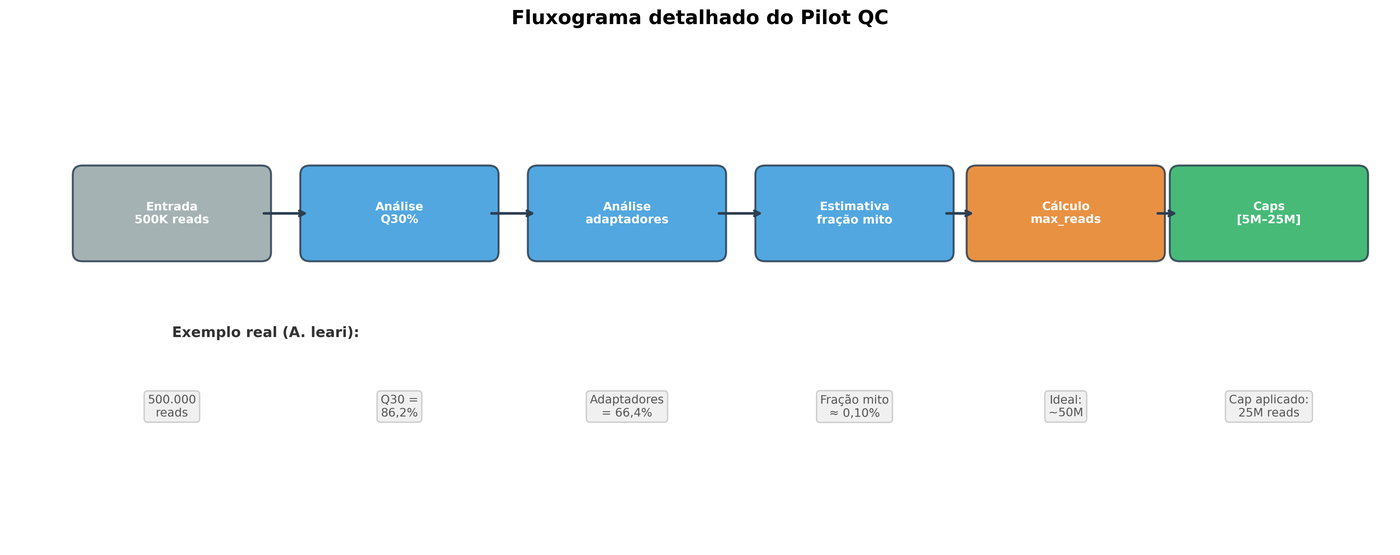
\includegraphics[width=0.85\textwidth]{imagens/pilot_qc_detalhado.png}
    \caption{Fluxograma de decisão do Pilot QC: análise de Q30\%, taxa de adaptadores e fração mitocondrial estimada para cálculo automático do número ideal de leituras, com caps entre 5M e 25M.}
    \label{fig:pilot_qc}
\end{figure}

\section{Controle de Qualidade e Pré-processamento}

Após a aquisição e organização dos dados de sequenciamento, a etapa seguinte do pipeline consiste na avaliação da qualidade das leituras e na aplicação de procedimentos de filtragem. Essa fase é essencial para assegurar que apenas dados confiáveis avancem para a montagem do genoma mitocondrial, evitando que artefatos técnicos comprometam a acurácia do resultado final.

O primeiro passo é a execução do FastQC v0.12.1, que gera relatórios interativos em HTML contendo métricas fundamentais para a avaliação da qualidade das leituras. Em seguida, é aplicado o Trim Galore v0.6.10 (que integra o Cutadapt v4.6), com parâmetros de qualidade Phred mínimo de 20 e comprimento mínimo de leitura de 50~bp para remoção de adaptadores e bases de baixa qualidade. No módulo implementado, o número de threads de CPU foi deliberadamente limitado a 2 para evitar ultrapassar a alocação de CPU no container, dado que o Trim Galore gera internamente threads adicionais para compressão (pigz) e para o próprio Cutadapt.

Além de aumentar a confiabilidade biológica das leituras, o pré-processamento contribui significativamente para a redução do volume de dados. Na execução para a arara-azul-de-lear, por exemplo, o Trim Galore detectou adaptadores Illumina TruSeq em 81,4\% das leituras, e após o trimming, 71,9\% das bases foram mantidas --- uma redução de volume de $\sim$28\%.

\section{Montagem do Mitogenoma}

A montagem do genoma mitocondrial constitui a etapa central do pipeline, pois é nela que se obtém a sequência circular completa que serve de base para a anotação funcional e análises comparativas. Para essa finalidade é utilizado o NOVOPlasty v4.3.1, um dos montadores mais consolidados para organelas \cite{dierckxsens2017}.

No pipeline implementado, o módulo NOVOPlasty incorpora diversas melhorias em relação ao uso padrão da ferramenta:

\begin{enumerate}
    \item \textbf{Múltiplos k-mers}: o parâmetro \texttt{novoplasty\_kmers} permite definir uma lista de valores de k-mer a serem tentados em sequência (e.g., \texttt{'39,33'}). O pipeline experimenta cada um até obter circularização;
    \item \textbf{Re-seeding automático}: para cada k-mer, caso a primeira execução não circularize, o maior contig obtido é automaticamente extraído e utilizado como nova semente em até 5 iterações (configurável);
    \item \textbf{Liberação de espaço}: após a montagem, os arquivos FASTQ trimados são automaticamente deletados para economizar espaço em disco, comportamento crucial para execuções com dados volumosos.
\end{enumerate}

A seleção dos valores de k-mer segue as recomendações do próprio NOVOPlasty \cite{dierckxsens2017}, que aceita valores ímpares no intervalo de 21 a 39. Valores maiores de k-mer (como 39) favorecem a \textbf{especificidade} da montagem --- cada k-mer é mais longo e, portanto, menos ambíguo, reduzindo o risco de quimeras e extensões incorretas. Por outro lado, valores menores (como 33) aumentam a \textbf{sensibilidade}, permitindo extensões em regiões de menor cobertura ou maior divergência entre a semente e o genoma-alvo. Assim, a estratégia adotada neste pipeline inicia pelo valor máximo (39), que produz montagens mais confiáveis quando a cobertura e a qualidade dos dados são adequadas, e recorre ao valor menor (33) apenas se a circularização não for alcançada na primeira tentativa. Para a arara-azul-de-lear, a circularização ocorreu na primeira tentativa com k-mer 39, indicando que a cobertura de 306$\times$ e a qualidade do HiSeq X Ten foram suficientes para o valor mais restritivo. Já para \textit{D.~bifasciatus}, a circularização ocorreu com k-mer 33, possivelmente refletindo diferenças na cobertura ou na composição nucleotídica do dataset.

\begin{figure}[H]
    \centering
    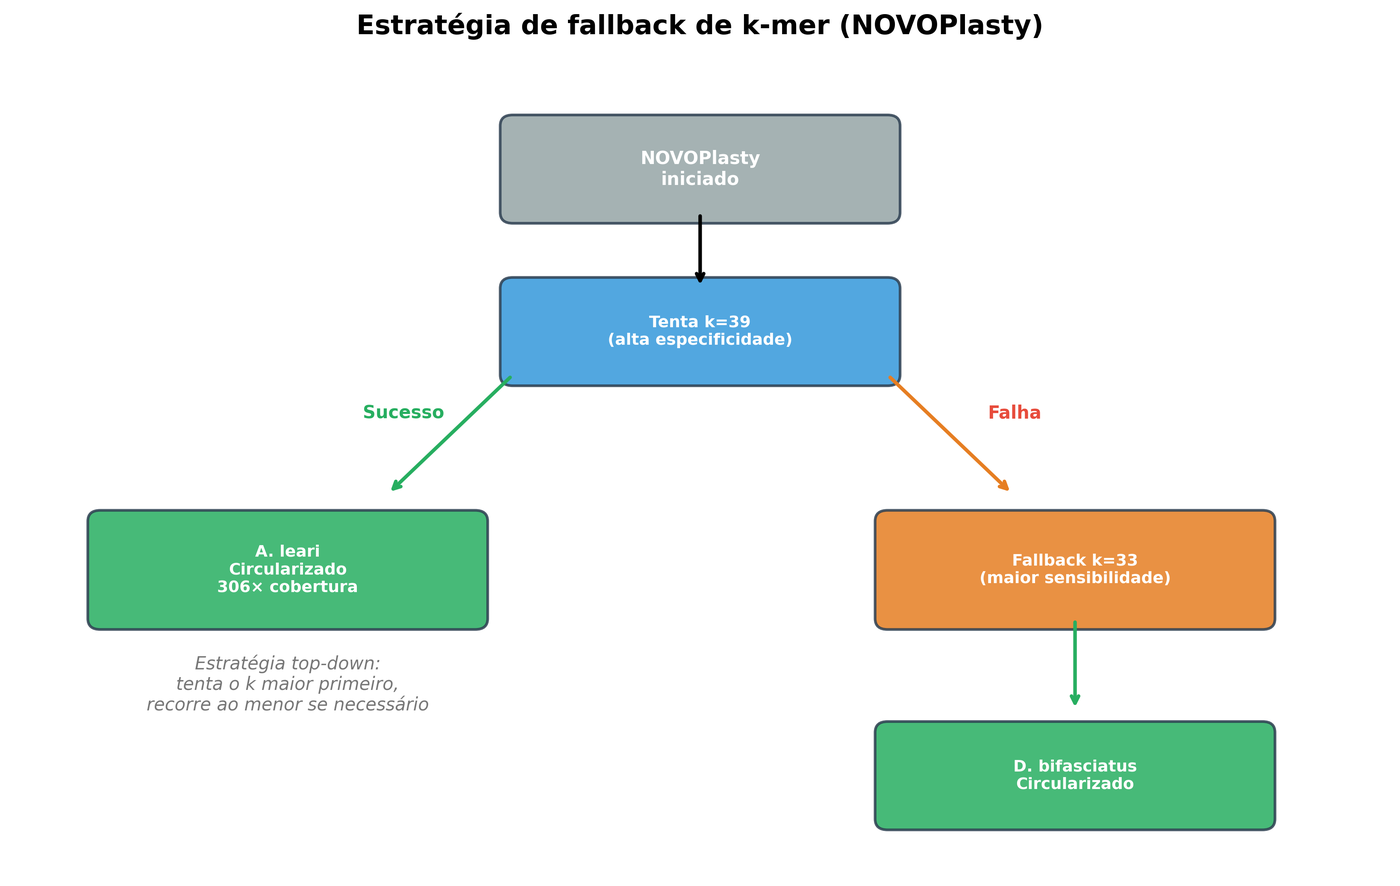
\includegraphics[width=0.85\textwidth]{imagens/kmer_fallback.png}
    \caption{Diagrama da lógica iterativa de k-mers: tentativa com k=39 (alta especificidade) seguida de \textit{fallback} para k=33 (maior sensibilidade) quando a circularização não é alcançada.}
    \label{fig:kmer_fallback}
\end{figure}

\textbf{Obtenção da semente (seed).} O NOVOPlasty requer uma sequência inicial conhecida para ancorar a extensão. A estratégia adotada neste trabalho consiste em: (i) identificar no NCBI uma espécie congênere ou filogeneticamente próxima que possua mitogenoma completo depositado; (ii) extrair o gene cox1 dessa referência, por ser o marcador mitocondrial mais conservado e amplamente disponível; e (iii) salvar a região em formato FASTA. Para a arara-azul-de-lear, foi utilizado o gene cox1 de \textit{A.~hyacinthinus} (NC\_082165.1, posições 5359--6906, 1.548~bp), espécie congênere cuja proximidade filogenética garante homologia suficiente para o seed-and-extend funcionar eficazmente. Para \textit{D.~bifasciatus}, foi utilizado o próprio cox1 da referência publicada (PZ143763.1, 1.560~bp). O repositório do pipeline inclui um guia detalhado para obtenção de sementes (\texttt{data/seeds/COMO\_OBTER\_SEMENTE.md}) e exemplos para sete espécies de diferentes grupos taxonômicos.

\textbf{Seleção do intervalo de tamanho (\texttt{genome\_range}).} O NOVOPlasty utiliza um intervalo esperado de tamanho do genoma para descartar extensões espúrias. A determinação desse intervalo segue a mesma lógica da semente: busca-se no NCBI o tamanho do mitogenoma de referência da espécie congênere mais próxima e aplica-se uma margem de $\pm$1.500--2.000~bp para acomodar variação interespecífica. Para a arara-azul-de-lear, a referência \textit{A.~hyacinthinus} (16.999~bp) resultou no intervalo 15.500--18.500~bp; para \textit{D.~bifasciatus}, a referência PZ143763.1 (16.805~bp) resultou em 15.000--18.500~bp.

\textbf{Parâmetro \texttt{insert\_size}.} O tamanho do inserto da biblioteca é parametrizado como 300~bp (valor padrão conservador para preparações Illumina). O NOVOPlasty utiliza esse valor como estimativa inicial, mas refina-o automaticamente durante a montagem --- no caso da arara-azul-de-lear, o inserto real medido foi de 213~bp, sem impacto na qualidade da circularização.

\section{Anotação Funcional}

Concluída a etapa de montagem, procede-se à anotação funcional do genoma mitocondrial reconstruído, utilizando o MITOS2 v2.1.9 com o banco de dados RefSeq89m. A anotação é executada automaticamente pelo pipeline quando o parâmetro \texttt{mitos2\_db} está configurado, sendo condicional para permitir que a Fase 1 (montagem) opere independentemente.

O módulo MITOS2 recebe como entrada o arquivo FASTA da montagem circularizada e produz como saída: arquivo GFF3 com coordenadas dos genes, tabelas BED, sequências proteicas preditas (FAA), mapa linear do genoma (PNG) e plots de qualidade (PDF). Adicionalmente, o pipeline gera automaticamente diagramas SVG da estrutura secundária prevista para cada tRNA e rRNA identificado, utilizando o programa RNAplot do pacote ViennaRNA.

O código genético é parametrizado (\texttt{genetic\_code = 2} para vertebrados mitocondriais, \texttt{genetic\_code = 5} para invertebrados), permitindo que o mesmo pipeline seja utilizado para diferentes grupos taxonômicos sem modificação de código.

\section{Compilação dos Entregáveis}

Uma funcionalidade diferenciada do pipeline é a compilação automática de todos os produtos da análise em uma pasta organizada de entregáveis (\texttt{summary/}), pronta para apresentação acadêmica ou submissão a bancos de dados. Essa etapa é executada pelo módulo \texttt{COMPILE\_SUMMARY}, que integra três scripts Python:

\begin{enumerate}
    \item \textbf{\texttt{gff2genbank.py}} --- Converte a anotação GFF3 do MITOS2 para o formato feature table (\texttt{.tbl}) do GenBank, com tratamento especial para o frameshift do ND3 em aves (uso de \texttt{join()} e \texttt{/exception=ribosomal slippage});
    \item \textbf{\texttt{generate\_genbank.py}} --- Gera o GenBank Flat File (\texttt{.gbk}) e o mapa circular do genoma (SVG e PDF) via Biopython GenomeDiagram \cite{cock2009};
    \item \textbf{\texttt{compile\_summary.py}} --- Reúne e organiza todos os arquivos em uma estrutura numerada.
\end{enumerate}

Os entregáveis gerados pelo pipeline são apresentados na Tabela~\ref{tab:entregaveis}.

\begin{longtable}{@{}clp{9cm}@{}}
\caption{Categorias de entregáveis gerados automaticamente pelo pipeline.}
\label{tab:entregaveis} \\
\toprule
\textbf{\#} & \textbf{Arquivo} & \textbf{Conteúdo} \\
\midrule
\endfirsthead
\caption[]{Categorias de entregáveis (continuação).} \\
\toprule
\textbf{\#} & \textbf{Arquivo} & \textbf{Conteúdo} \\
\midrule
\endhead
\bottomrule
\endfoot
01 & \texttt{01\_genome\_assembly.fasta} & Mitogenoma circularizado completo \\
\addlinespace
02 & \texttt{02\_coding\_genes\_nt.fasta} & 13 CDS em nucleotídeos \\
\addlinespace
03 & \texttt{03\_coding\_genes\_aa.fasta} & 13 CDS em aminoácidos \\
\addlinespace
04 & \texttt{04\_ribosomal\_genes.fasta} & 12S + 16S rRNA \\
\addlinespace
05 & \texttt{05\_transport\_genes.fasta} & 22 tRNAs \\
\addlinespace
06 & \texttt{06\_gene\_positions.tsv} & Posição física de todos os genes \\
\addlinespace
07 & \texttt{07\_start\_stop\_codons.tsv} & Start/Stop codons dos CDS \\
\addlinespace
08 & \texttt{08\_trna\_anticodons.tsv} & Anticódons dos tRNAs \\
\addlinespace
09 & \texttt{09\_circular\_map.svg/pdf} & Mapa circular colorido por grupo funcional \\
\addlinespace
10 & \texttt{10\_annotation.gff} & Anotação GFF3 completa \\
\addlinespace
11 & \texttt{structure\_svgs/} & 22 SVGs de tRNA + 2 SVGs de rRNA \\
\addlinespace
12 & \texttt{genbank\_submission/} & \texttt{.gbk} + \texttt{.tbl} + \texttt{.fsa} para GenBank \\
\addlinespace
13 & \texttt{13\_gene\_order.txt} & Ordem gênica linear \\
\addlinespace
14 & \texttt{quality\_plots/} & Plots de qualidade do MITOS2 \\
\end{longtable}

Todos os scripts são genéricos --- recebem o nome da espécie como parâmetro (\texttt{-{}-organism}) e derivam automaticamente o identificador de sequência (e.g., ``Anodorhynchus leari'' $\rightarrow$ seqid \texttt{A\_leari}), tornando o pipeline reutilizável para qualquer táxon.

\section{Automação e Reprodutibilidade}

A automação do pipeline e a padronização de sua execução representam os principais diferenciais desta proposta em relação a abordagens convencionais de montagem de genomas mitocondriais. Mais do que reunir ferramentas em sequência, busca-se disponibilizar um fluxo de trabalho que possa ser aplicado por diferentes grupos de pesquisa em distintos ambientes computacionais, assegurando consistência analítica, transparência metodológica e facilidade de reutilização.

Para atingir esse objetivo, cada etapa do pipeline foi encapsulada em containers Docker, garantindo que as ferramentas operem em ambientes controlados e reprodutíveis, independentemente do sistema em que forem executadas \cite{merkel2014}. A orquestração pelo Nextflow automatiza a execução dos processos, gerencia dependências e possibilita paralelização quando aplicável. O sistema ainda permite a retomada da análise a partir do ponto de falha (via \texttt{-resume}), evitando reprocessamento desnecessário e aumentando a eficiência computacional \cite{ditommaso2017}.

Todo o código-fonte do workflow está disponibilizado em repositório público no GitHub, acompanhado de documentação detalhada, guia de execução e exemplos de uso. Essa prática de ciência aberta não apenas reforça a transparência metodológica, mas também incentiva a adaptação e o aprimoramento do pipeline por outros pesquisadores, em consonância com iniciativas comunitárias como o nf-core \cite{ewels2020}.

\begin{figure}[H]
    \centering
    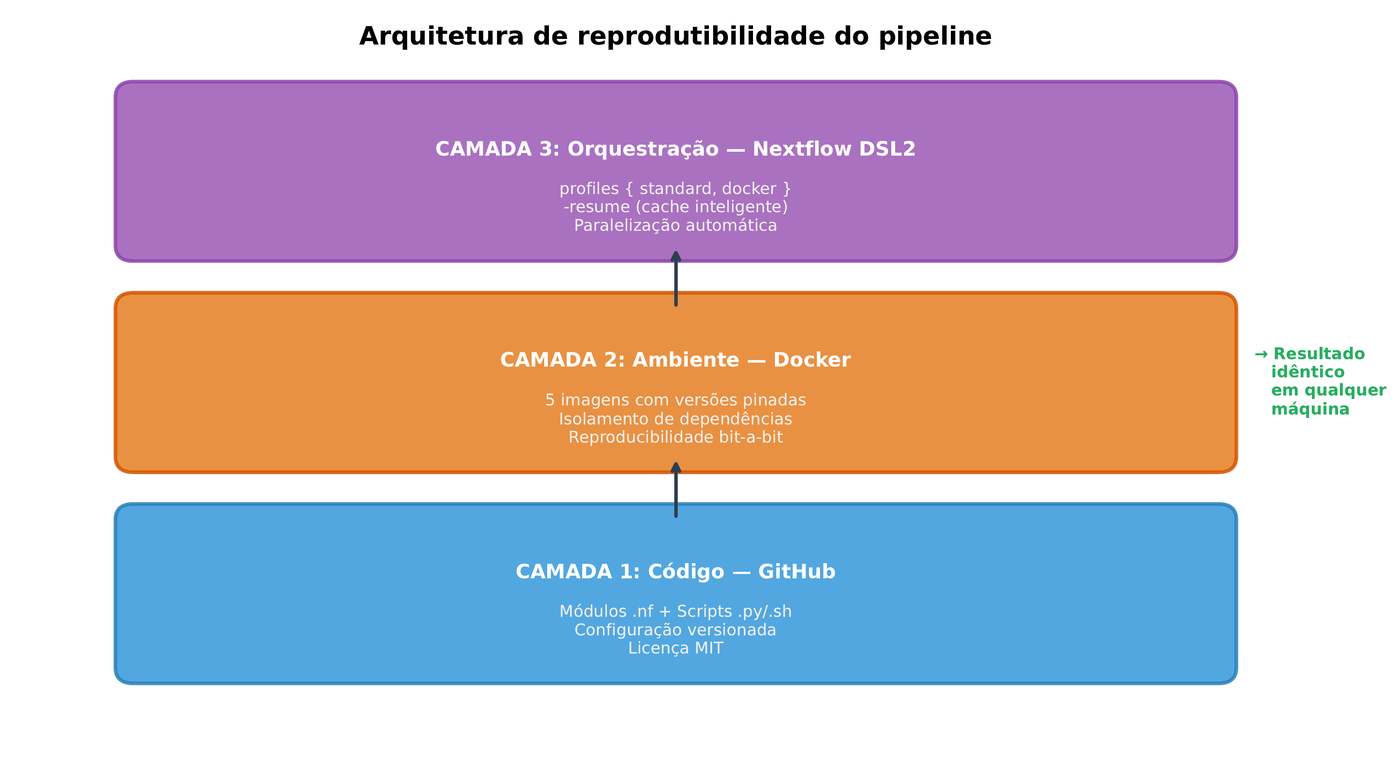
\includegraphics[width=0.85\textwidth]{imagens/camadas_reprodutibilidade.png}
    \caption{Três camadas de reprodutibilidade do pipeline: (1) código-fonte no GitHub, (2) ambiente isolado via Docker com versões pinadas, (3) orquestração via Nextflow DSL2.}
    \label{fig:camadas_reprodutibilidade}
\end{figure}

% ============================================================================
% CAPÍTULO 5 — RESULTADOS E DISCUSSÃO
% ============================================================================

\chapter{Resultados e Discussão}
\label{cap:resultados}

Este capítulo apresenta os resultados obtidos com a aplicação do pipeline desenvolvido, organizados segundo as etapas do fluxo de trabalho. Diferentemente da versão anterior deste trabalho, que apresentava resultados esperados de natureza projetiva, os dados aqui descritos são produtos reais de execuções completas do pipeline, validando sua funcionalidade e robustez.

\section{Execuções Realizadas}

O pipeline foi executado para duas espécies, com objetivos complementares. A Tabela~\ref{tab:execucoes} sintetiza os parâmetros e configurações utilizados em cada execução.

\begin{longtable}{@{}p{3.8cm}p{5.2cm}p{5.2cm}@{}}
\caption{Parâmetros de execução do pipeline para as duas espécies analisadas.}
\label{tab:execucoes} \\
\toprule
\textbf{Parâmetro} & \textbf{\textit{Anodorhynchus leari}} & \textbf{\textit{Diploprion bifasciatus}} \\
\midrule
\endfirsthead
\caption[]{Parâmetros de execução do pipeline (continuação).} \\
\toprule
\textbf{Parâmetro} & \textbf{\textit{A.~leari}} & \textbf{\textit{D.~bifasciatus}} \\
\midrule
\endhead
\bottomrule
\endfoot
Objetivo & Objeto principal do TCC & Validação do pipeline \\
\addlinespace
Dataset SRA & SRR28399504 & SRR36182901 \\
\addlinespace
Plataforma & Illumina HiSeq X Ten & NovaSeq X Plus \\
\addlinespace
Leituras & 118,5M $\times$ 150 bp & 12,0M $\times$ 151 bp \\
\addlinespace
Semente & cox1 \textit{A.~hyacinthinus} (NC\_082165.1, 1.548 bp) & cox1 \textit{D.~bifasciatus} (PZ143763.1, 1.560 bp) \\
\addlinespace
\texttt{genome\_range} & 15.500--18.500 bp & 15.000--18.500 bp \\
\addlinespace
K-mers & 39, 33 & 33 \\
\addlinespace
Código genético & 2 (vertebrado) & 2 (vertebrado) \\
\addlinespace
MITOS2 & Sim (RefSeq89m) & Não (perfil de teste sem banco) \\
\addlinespace
Perfil & \texttt{-profile a\_leari} & \texttt{-profile test} \\
\end{longtable}

\section{Aquisição e Preparo dos Dados}

Para a arara-azul-de-lear, o download via \texttt{prefetch} obteve o arquivo \texttt{.sra} de 11~GB, que foi convertido pelo \texttt{fasterq-dump} em dois arquivos FASTQ de aproximadamente 43,5~GB cada (R1 e R2). Após a truncagem para 20 milhões de leituras, os arquivos foram reduzidos para $\sim$7,4~GB cada, representando uma economia de 83\% em volume de dados processados sem qualquer prejuízo à montagem, dada a redundância intrínseca dos dados de genoma total.

\begin{figure}[H]
    \centering
    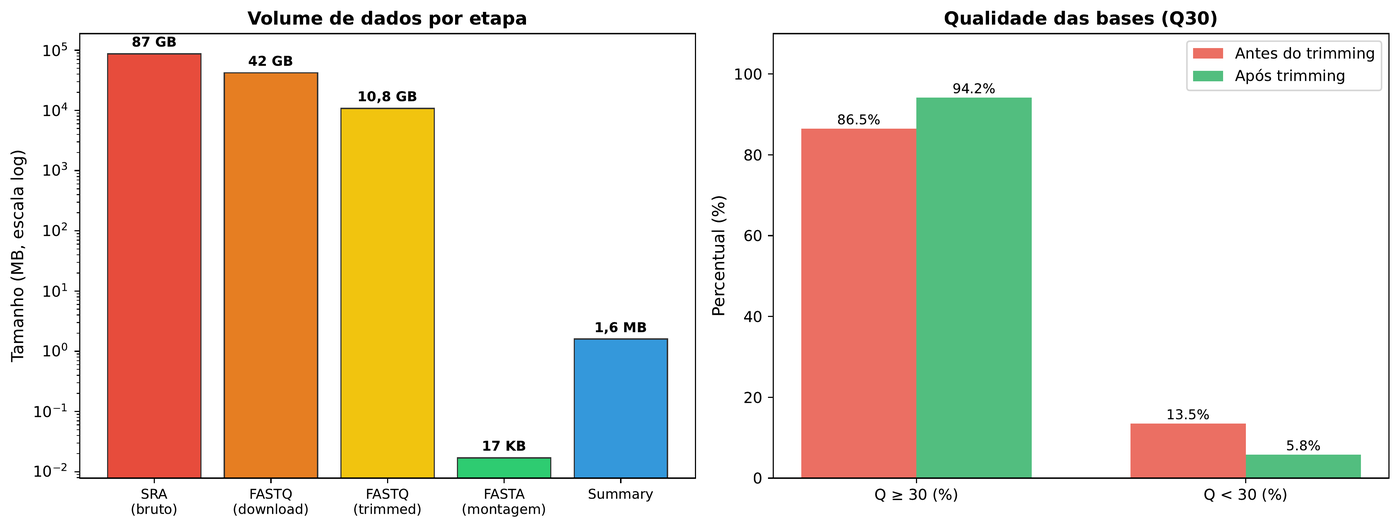
\includegraphics[width=0.85\textwidth]{imagens/reducao_volume_composicao.png}
    \caption{Redução de volume em cada etapa do pipeline para a arara-azul-de-lear: tamanho dos arquivos por etapa (esquerda) e composição de bases após trimming (direita).}
    \label{fig:reducao_volume}
\end{figure}

Para \textit{D.~bifasciatus}, o dataset compacto (12M reads, $\sim$1,2~GB) foi processado integralmente sem necessidade de truncagem, utilizando como semente o gene cox1 da própria referência publicada (PZ143763.1, 1.560 bp) e \texttt{genome\_range} de 15.000--18.500 bp.

\section{Controle de Qualidade e Pré-processamento}

Os relatórios do FastQC para a arara-azul-de-lear indicaram qualidade \textit{per-base} consistente (medianas superiores a Phred 30 ao longo de toda a extensão das leituras), padrão esperado para dados HiSeq X Ten. O Trim Galore identificou adaptadores Illumina TruSeq em 81,4\% das leituras e, após o trimming, manteve 71,9\% das bases originais. Esse percentual elevado de adaptador é atribuído ao tamanho curto dos insertos da biblioteca, característico de preparações para HiSeq X Ten, em que os fragmentos frequentemente ultrapassam o comprimento das leituras.

\begin{figure}[H]
    \centering
    \begin{minipage}[t]{0.48\textwidth}
        \centering
        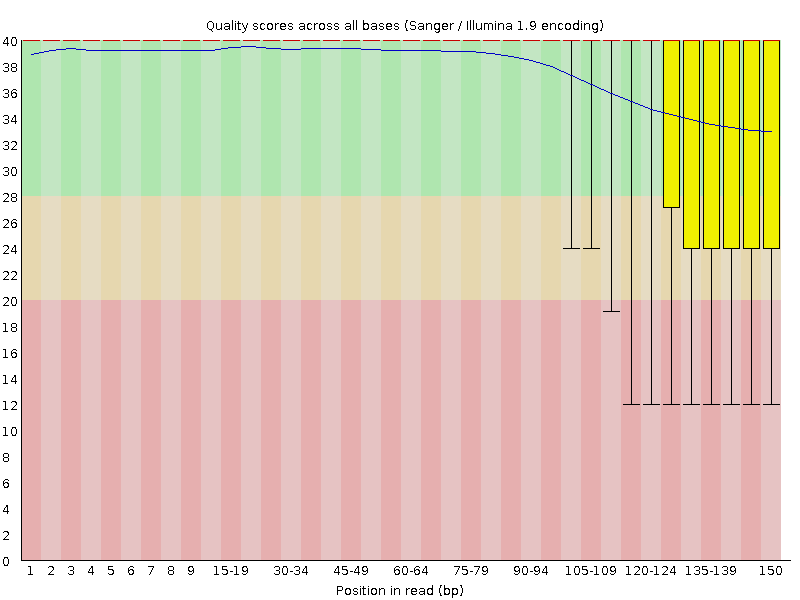
\includegraphics[width=\textwidth]{imagens/fastqc_R1_quality.png}
    \end{minipage}
    \hfill
    \begin{minipage}[t]{0.48\textwidth}
        \centering
        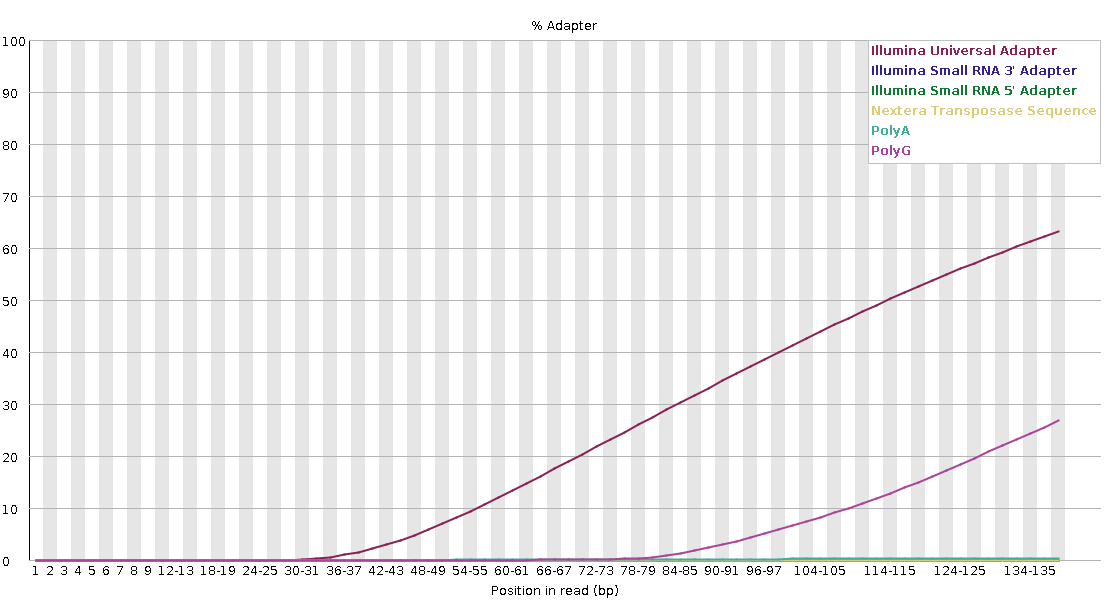
\includegraphics[width=\textwidth]{imagens/fastqc_R1_adapter.png}
    \end{minipage}

    \vspace{0.3cm}

    \begin{minipage}[t]{0.48\textwidth}
        \centering
        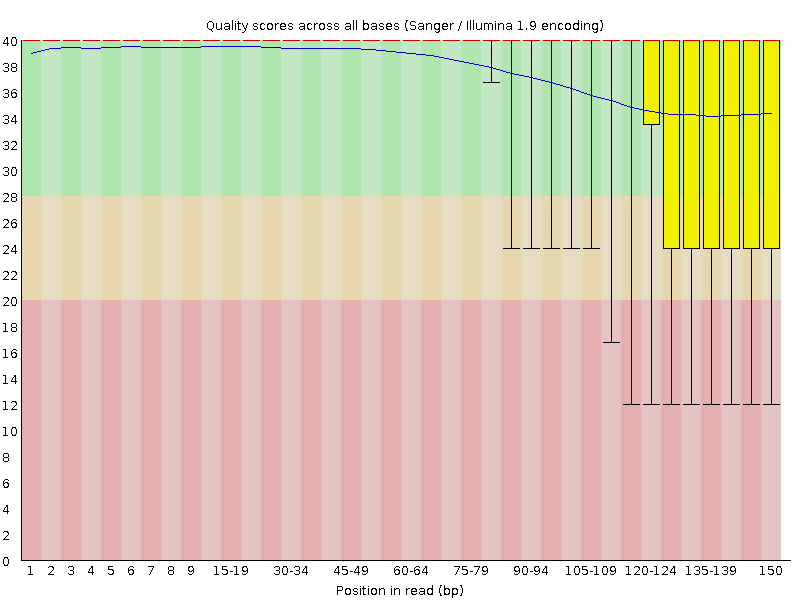
\includegraphics[width=\textwidth]{imagens/fastqc_R2_quality.png}
    \end{minipage}
    \hfill
    \begin{minipage}[t]{0.48\textwidth}
        \centering
        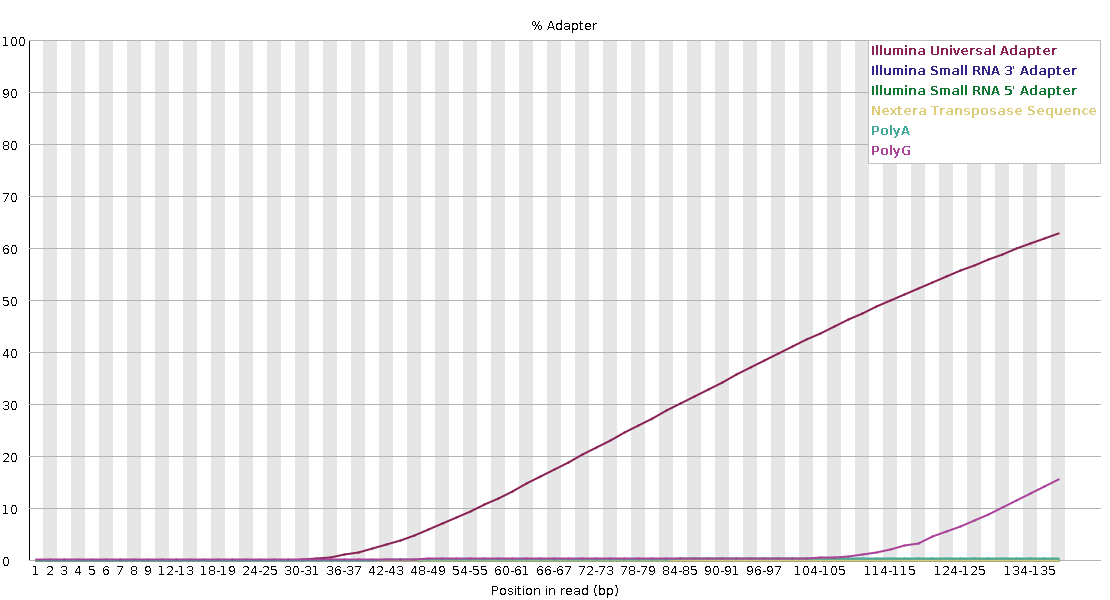
\includegraphics[width=\textwidth]{imagens/fastqc_R2_adapter.png}
    \end{minipage}
    \caption{Relatórios FastQC para a arara-azul-de-lear. Acima: R1 --- qualidade \textit{per-base} (esq.) e conteúdo de adaptadores (dir.). Abaixo: R2 --- qualidade \textit{per-base} (esq.) e conteúdo de adaptadores (dir.).}
    \label{fig:fastqc}
\end{figure}

\section{Montagem do Mitogenoma}

A montagem pelo NOVOPlasty resultou em genomas mitocondriais circularizados para ambas as espécies. A Tabela~\ref{tab:montagem} apresenta as métricas de montagem obtidas.

\begin{table}[H]
\centering
\caption{Métricas de montagem do mitogenoma para as duas espécies analisadas.}
\label{tab:montagem}
\footnotesize
\begin{tabular}{@{}lp{4.5cm}p{5cm}@{}}
\toprule
\textbf{Métrica} & \textbf{\textit{A.~leari}} & \textbf{\textit{D.~bifasciatus}} \\
\midrule
Tamanho & 16.986 bp & $\sim$16.800 bp (circularizado) \\
Circularização & Sim & Sim \\
K-mer ótimo & 39 & 33 \\
Cobertura média & 306$\times$ & não medida (dataset completo) \\
Reads alinhadas & 34.644 / 20.285.220 (0,17\%) & --- \\
Insert size medido & 213 bp (parametrizado: 300) & --- \\
Referência & 16.999 bp (\textit{A.~hyacinthinus}) --- $\Delta$ 13 bp & 16.805 bp (PZ143763.1) --- $\Delta$ $\sim$5 bp \\
\bottomrule
\end{tabular}
\end{table}

Para \textit{D.~bifasciatus}, o dataset compacto (12M reads, $\sim$1,2~GB) foi processado integralmente sem truncagem; a circularização ocorreu na primeira tentativa com k-mer 33. A etapa de anotação funcional (MITOS2) não foi executada para esta espécie no perfil de teste, que foi configurado sem o parâmetro \texttt{mitos2\_db} para demonstrar a modularidade do pipeline --- a Fase 1 (montagem) opera independentemente da Fase 2 (anotação). A validação da montagem pode ser realizada por BLAST contra a referência PZ143763.1.

O resultado da arara-azul-de-lear merece destaque: o genoma montado de 16.986 bp difere em apenas 13 pares de bases do mitogenoma de referência de \textit{A.~hyacinthinus} (16.999 bp, NC\_082165.1), demonstrando alta congruência interespecífica esperada para o gênero \textit{Anodorhynchus}. A cobertura média de 306$\times$ é amplamente superior ao mínimo recomendado de 30--50$\times$ para montagens confiáveis \cite{dierckxsens2017}, conferindo alta confiabilidade ao resultado.

A proporção de leituras mitocondriais de 0,17\% é condizente com a estimativa teórica para dados de genoma total de aves, onde o número de cópias mitocondriais por célula é tipicamente na ordem de centenas a milhares, mas o genoma nuclear ($\sim$1,2~Gb em psitacídeos) é muito maior que o mitocondrial ($\sim$17~kb).

O log do NOVOPlasty reportou uma fração de subamostragem (\textit{subsampled fraction}) de 61,9\%, indicando que o algoritmo processou 61,9\% das leituras de entrada antes de obter a circularização. Esse valor reflete a eficiência do \textit{seed-and-extend}: como o NOVOPlasty constrói o genoma iterativamente a partir da semente, ele pode alcançar a montagem completa sem necessidade de processar todas as leituras disponíveis, resultando em economia computacional proporcional à fração não processada.

\begin{figure}[H]
    \centering
    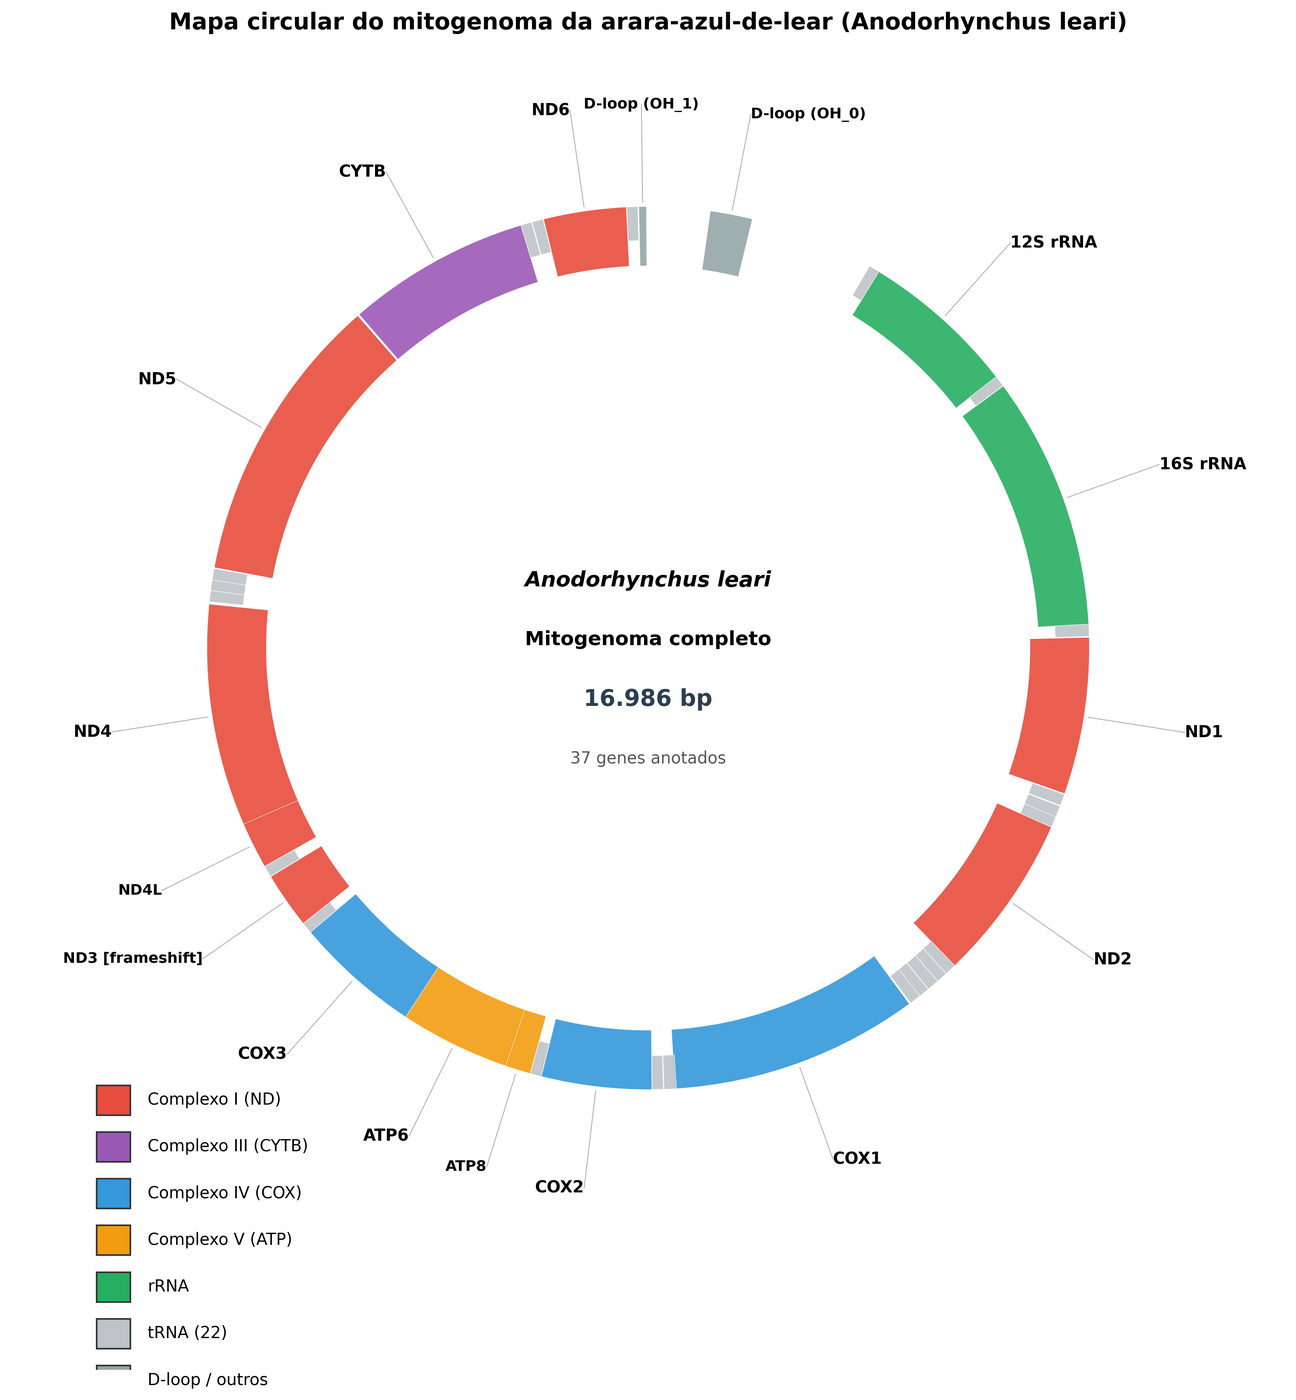
\includegraphics[width=0.70\textwidth]{imagens/mapa_circular_mitogenoma.png}
    \caption{Mapa circular do mitogenoma da arara-azul-de-lear (\textit{A.~leari}), mostrando a posição dos 37 genes (13 CDS, 22 tRNAs, 2 rRNAs) e a região controle (D-loop). Gerado automaticamente pelo pipeline via Biopython GenomeDiagram.}
    \label{fig:mapa_circular}
\end{figure}

\section{Anotação Funcional}

A anotação pelo MITOS2 identificou o conjunto completo de genes esperado para um genoma mitocondrial de ave, conforme apresentado na Tabela~\ref{tab:anotacao}.

\begin{table}[H]
\centering
\caption{Conteúdo gênico do mitogenoma da arara-azul-de-lear anotado pelo MITOS2.}
\label{tab:anotacao}
\begin{tabular}{@{}clp{9.5cm}@{}}
\toprule
\textbf{Tipo} & \textbf{Qtd.} & \textbf{Genes} \\
\midrule
CDS & 13 & nad1, nad2, nad3, nad4, nad4l, nad5, nad6, cox1, cox2, cox3, atp6, atp8, cob \\
\addlinespace
tRNA & 22 & tRNA-Phe, tRNA-Val, tRNA-Leu1, tRNA-Ile, tRNA-Gln, tRNA-Met, tRNA-Trp, tRNA-Ala, tRNA-Asn, tRNA-Cys, tRNA-Tyr, tRNA-Ser1, tRNA-Asp, tRNA-Lys, tRNA-Gly, tRNA-Arg, tRNA-His, tRNA-Ser2, tRNA-Leu2, tRNA-Glu, tRNA-Thr, tRNA-Pro \\
\addlinespace
rRNA & 2 & rrnS (12S), rrnL (16S) \\
\addlinespace
Origem de replicação & 2 & OH\_0, OH\_1 \\
\bottomrule
\end{tabular}
\end{table}

A ordem gênica identificada é compatível com o padrão conservado de Psittaciformes, corroborando a confiabilidade da montagem. A comparação com a anotação de \textit{A.~hyacinthinus} (NC\_082165.1) confirmou a conservação da organização gênica dentro do gênero. A completude e a consistência da anotação --- 13 CDS, 22 tRNAs com anticódons corretos, 2 rRNAs nas posições esperadas e nenhum gene truncado ou duplicado --- servem como validação biológica indireta da montagem: um genoma incorretamente circularizado ou contendo inserções e deleções artifactuais produziria genes com códons de parada prematuros, tRNAs com estruturas secundárias anômalas ou regiões intergênicas atipicamente longas --- nenhum dos quais foi observado.

\subsection{Caso Especial --- Frameshift do ND3}

Um aspecto biologicamente relevante revelado pela anotação é o tratamento do gene ND3. O MITOS2 reportou este gene como dois ORFs distintos (\texttt{nad3\_0} e \texttt{nad3\_1}) com sobreposição de 5~bp, refletindo o \textit{frameshift insertion} documentado por \citeonline{mindell1998} em genomas mitocondriais de aves. Esse fenômeno, em que uma inserção de $\sim$1 nucleotídeo altera o quadro de leitura no interior do gene, é corrigido \textit{in vivo} por mecanismos de \textit{programmed ribosomal frameshift} ou edição do mRNA. Na referência \textit{A.~hyacinthinus} (NC\_082165.1), o ND3 é anotado com \texttt{join()}:

\begin{lstlisting}
CDS   join(9504..9677,9679..9854)
      /gene="ND3"
      /note="frameshift mechanism unknown (Mindell et al., 1998)"
\end{lstlisting}

Para a conversão dos resultados ao formato GenBank Flat File, o script \texttt{gff2genbank\allowbreak.py} do pipeline detecta automaticamente a presença de \texttt{nad3\_0} e \texttt{nad3\_1} e os unifica em um único CDS com \texttt{join()}, aplicando o qualificador \texttt{/exception=\allowbreak ribosomal\allowbreak{} slippage} --- exatamente como exigido pelo GenBank para submissão. Quando a espécie não apresenta esse \textit{frameshift} (e.g., invertebrados), o ND3 é anotado normalmente como um CDS contínuo.

% Tabela de posição física dos genes será apresentada no Capítulo 6.

\begin{figure}[H]
    \centering
    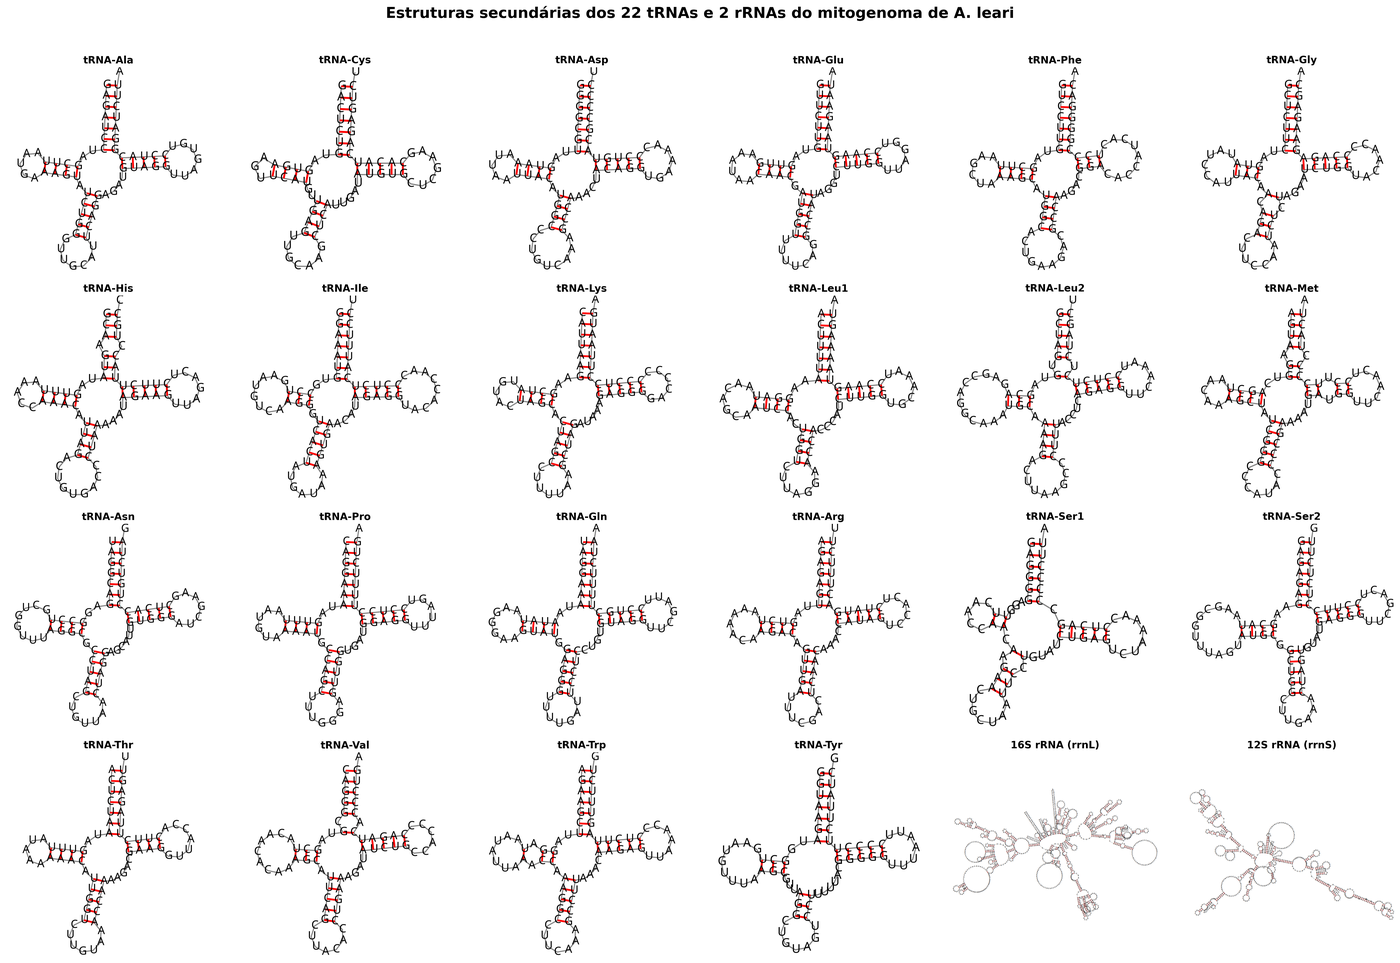
\includegraphics[width=\textwidth]{imagens/painel_trna_rrna.png}
    \caption{Painel com estruturas secundárias dos 22 tRNAs e 2 rRNAs preditos pelo MITOS2/RNAplot para \textit{A.~leari}. Nota-se a ausência do braço DHU no tRNA-Ser(AGY), padrão conservado em metazoários.}
    \label{fig:painel_trna_rrna}
\end{figure}

\section{Compilação dos Entregáveis e Formato GenBank}

O módulo COMPILE\_SUMMARY reuniu automaticamente todos os produtos da análise em uma pasta organizada com 14 categorias de entregáveis, conforme detalhado na Tabela da Seção~4.11. Destaca-se a geração automática do GenBank Flat File (\texttt{.gbk}), que é o formato padrão exigido pelo NCBI para submissão de genomas. O arquivo gerado para a arara-azul-de-lear contém:

\begin{lstlisting}[caption={Trecho do GenBank Flat File gerado pelo pipeline para \textit{A.~leari}.},label={lst:genbank}]
LOCUS       A_leari                16986 bp    DNA     circular VRT 12-APR-2026
DEFINITION  Anodorhynchus leari mitochondrion, complete genome.
ACCESSION   A_leari
VERSION     A_leari
FEATURES             Location/Qualifiers
     source          1..16986
                     /organism="Anodorhynchus leari"
                     /organelle="mitochondrion"
                     /mol_type="genomic DNA"
     ...
     CDS             join(10919..11098,11094..11267)
                     /gene="ND3"
                     /exception="ribosomal slippage"
                     /note="programmed frameshift; Mindell et al. (1998)"
     ...
ORIGIN
        1 gtttacgcta taaagcgtta gatataactg ...
//
\end{lstlisting}

Esse formato pode ser diretamente submetido ao GenBank via \texttt{table2asn} ou carregado em ferramentas de visualização como OGDRAW para geração de mapas circulares de alta qualidade.

\section{Análise de Desempenho e Eficiência Computacional}

A avaliação de desempenho de um pipeline bioinformático é essencial para determinar sua viabilidade prática em diferentes cenários de uso --- desde laptops pessoais até servidores de computação em nuvem. Em bioinformática, pipelines frequentemente processam volumes massivos de dados (dezenas a centenas de gigabytes), e compreender onde o tempo e os recursos computacionais são consumidos permite identificar gargalos, dimensionar infraestrutura adequada e estimar custos operacionais. Essa análise é particularmente relevante para laboratórios com recursos limitados, que precisam avaliar se dispõem de hardware suficiente antes de iniciar uma execução.

Nesta seção, são apresentadas métricas detalhadas de execução do pipeline para a arara-azul-de-lear, incluindo tempo, consumo de CPU, memória RAM e operações de entrada/saída (I/O) --- isto é, volume de dados lidos e escritos em disco --- por etapa. A partir dessas métricas, discutem-se a eficiência de cada módulo, a identificação de gargalos, o impacto do pré-processamento na qualidade da montagem, e o custo estimado de execução em infraestrutura de nuvem.

A execução foi realizada em um laptop com processador Intel Core i7-1165G7 (4 núcleos físicos, 8 threads via \textit{hyperthreading}, frequência base de 2,80~GHz), 16~GB de memória RAM DDR4 e armazenamento em estado sólido (SSD NVMe). O tempo total decorrido --- também chamado \textit{wall-clock time}, que mede o tempo real percebido pelo usuário, incluindo esperas por I/O e rede --- foi de \textbf{56 minutos e 42 segundos}, com consumo acumulado de \textbf{4,2 horas de CPU} (tempo efetivo de processamento somado de todos os núcleos). A Tabela~\ref{tab:desempenho} apresenta as métricas detalhadas por etapa.

\begin{table}[H]
\centering
\caption{Métricas de desempenho por etapa do pipeline (execução arara-azul-de-lear, 50M reads).}
\label{tab:desempenho}
\resizebox{\textwidth}{!}{%
\begin{tabular}{@{}lrrrrrr@{}}
\toprule
\textbf{Etapa} & \textbf{Tempo (min)} & \textbf{\% total} & \textbf{CPU (\%)} & \textbf{RAM pico (GB)} & \textbf{I/O leitura} & \textbf{I/O escrita} \\
\midrule
SRA\_PILOT & 1,9 & 3,4\% & 113\% & 0,15 & 3,4 MB & 474 MB \\
SRA\_DOWNLOAD & 33,8 & 59,6\% & 586\% & 0,43 & 160 GB & 250 GB \\
FASTQC & 7,6 & 13,4\% & 1966\% & 1,04 & 34,7 GB & 4,8 MB \\
TRIM\_GALORE & 12,2 & 21,5\% & 2084\% & 0,12 & 68,5 GB & 53,4 GB \\
NOVOPLASTY & 4,5 & 8,0\% & 827\% & 11,11 & 18 GB & 28 KB \\
MITOS2 & 4,1 & 7,2\% & 1033\% & 0,41 & 222 MB & 45 MB \\
\midrule
\textbf{Total} & \textbf{56,7} & \textbf{100\%} & --- & --- & --- & --- \\
\bottomrule
\end{tabular}}%
\end{table}

\begin{figure}[H]
    \centering
    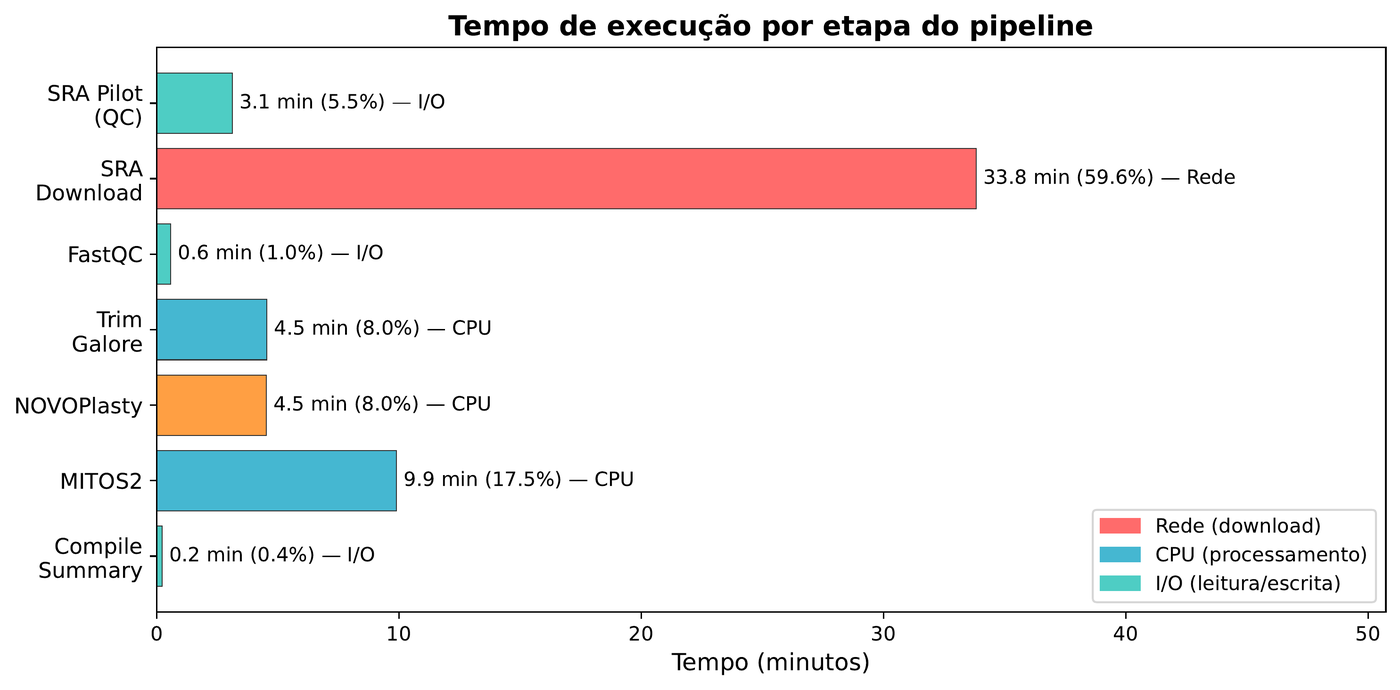
\includegraphics[width=0.85\textwidth]{imagens/tempo_etapas_pipeline.png}
    \caption{Tempo de execução por etapa do pipeline para a arara-azul-de-lear, com anotação da porcentagem do tempo total e classificação por tipo de operação (I/O-bound vs CPU-bound).}
    \label{fig:tempo_etapas}
\end{figure}

\subsection{Gargalo de I/O: Download e Conversão SRA}

O download do SRA é o gargalo dominante, consumindo \textbf{59,6\% do tempo total}. A etapa engloba três operações sequenciais: \texttt{prefetch} (download do arquivo \texttt{.sra} comprimido, $\sim$11~GB), \texttt{fasterq-dump} (conversão para FASTQ, gerando $\sim$87~GB intermediários para 118M reads), e truncamento via \texttt{head} (redução para 50M reads). O volume total de I/O desta etapa (160~GB lidos + 250~GB escritos) confirma que a conversão de formato é o fator limitante, não a rede --- o \texttt{fasterq-dump} precisa descomprimir e reescrever todos os 118M reads mesmo que apenas 50M sejam necessários, pois o formato \texttt{.sra} não permite acesso aleatório por read.

Esse comportamento reforça a importância do módulo Pilot QC, que utiliza \texttt{fastq-dump\allowbreak{} -X\allowbreak{} 500000} para amostrar apenas as primeiras 500K reads diretamente da origem (sem download completo), consumindo apenas 1,9 minutos e 474~MB. Sem o Pilot, o usuário precisaria decidir arbitrariamente quantas reads baixar, arriscando sub ou superamostragem.

\subsection{Eficiência do Pré-processamento}

O Trim Galore consumiu 12,2 minutos (21,5\% do tempo), processando 100 milhões de reads (50M pares). A taxa de remoção de adaptadores foi de 81,4\% (R1) e 80,8\% (R2), com remoção de bases por qualidade inferior a 1\% (74M bp em R1, 51M bp em R2). Do total de 50M pares, 3.711.983 (7,42\%) foram removidos por ficarem abaixo de 50~bp após trimming --- indicando dímeros de adaptador. O volume de dados foi reduzido de 15~Gbp brutos para 10,78~Gbp filtrados (71,9\% de retenção em bases).

Uma questão pertinente é: \textbf{o trimming é necessário ou é perda de tempo?} A resposta é inequívoca: com 81,4\% dos reads contendo adaptador Illumina TruSeq, executar a montagem sem trimming resultaria em k-mers quiméricos (parte sequência biológica, parte adaptador sintético) que impediriam a extensão correta do grafo de Bruijn. Os 12,2 minutos de trimming ($\sim$21\% do pipeline) previnem artefatos de montagem que poderiam resultar em falha de circularização ou contigs espúrios. Em contraste, a montagem pós-trimming completou em apenas 4,5 minutos, com circularização na primeira tentativa.

O FASTQC rodou em paralelo com o Trim Galore (ambos consomem os mesmos FASTQs), não adicionando tempo ao caminho crítico. O pico de memória do FASTQC (1,04~GB) é significativo para máquinas com pouca RAM, mas justificável pela geração de relatórios de qualidade essenciais para verificação posterior.

\subsection{Anomalia de Memória do NOVOPlasty}

O NOVOPlasty apresentou o maior consumo de memória entre todas as etapas: \textbf{11,1~GB de RAM} (pico). Embora inferior aos 16~GB de memória física do sistema, esse valor --- somado ao consumo do sistema operacional, Docker e demais processos residentes ($\sim$3--4~GB) --- aproximou-se do limite total, resultando em uso pontual de \textit{swap}. O alto consumo decorre da construção do \textit{hash} de k-mers em memória para as 46M reads remanescentes. O NOVOPlasty, escrito em Perl, não possui gerenciamento granular de memória, e o parâmetro \texttt{Max memory} (configurado como 12~GB) serve apenas como limite superior sugerido, não como restrição efetiva.

A fração ``subsampled'' de 22,93\% reportada no log indica que o NOVOPlasty sub-amostrou internamente os dados de entrada, processando efetivamente $\sim$10,6M reads dos 46,3M disponíveis. Mesmo com essa sub-amostragem, a cobertura final de 306$\times$ é 6$\times$ superior ao mínimo recomendado de 50$\times$ \cite{dierckxsens2017}. Esse é um indicador relevante: com metade das reads (25M em vez de 50M), a montagem provavelmente ainda seria bem-sucedida, com cobertura estimada de $\sim$150$\times$.

\textbf{Recomendação prática:} para execução em máquinas com menos de 8~GB de RAM, reduzir o \texttt{sra\_max\_reads} para 20M ou configurar \texttt{Max memory = 6} no perfil Nextflow. A qualidade da montagem não seria comprometida.

\subsection{Cascata de Redução de Dados}

Uma análise particularmente reveladora é a redução progressiva do volume de dados ao longo do pipeline. A Tabela~\ref{tab:cascata} apresenta essa cascata de redução.

\begin{table}[H]
\centering
\caption{Cascata de redução de dados ao longo do pipeline.}
\label{tab:cascata}
\begin{tabular}{@{}lrrr@{}}
\toprule
\textbf{Etapa} & \textbf{Volume} & \textbf{Fator de redução} & \textbf{Acumulado} \\
\midrule
SRA completo (118,5M reads) & $\sim$87 GB & --- & 1$\times$ \\
Após truncamento (50M reads) & $\sim$42 GB & 2,1$\times$ & 2,1$\times$ \\
Após trimming (46,3M reads) & $\sim$10,8 GB & 3,9$\times$ & 8,1$\times$ \\
Montagem circularizada & 17 KB & 635.000$\times$ & $\sim$5.100.000$\times$ \\
Summary (todos entregáveis) & 1,6 MB & --- & $\sim$54.000$\times$ \\
\bottomrule
\end{tabular}
\end{table}

O dado original (87~GB de FASTQ bruto) é reduzido em mais de \textbf{cinco milhões de vezes} até a montagem final (17~KB). Essa cascata demonstra que a maior parte do sequenciamento WGS é irrelevante para o genoma mitocondrial --- apenas 0,17\% das reads alinham ao mitogenoma. A existência do Pilot QC como primeira etapa evita o download desnecessário: em vez de baixar os 87~GB completos, o pipeline determina automaticamente que 50M reads ($\sim$42~GB) são suficientes.

\begin{figure}[H]
    \centering
    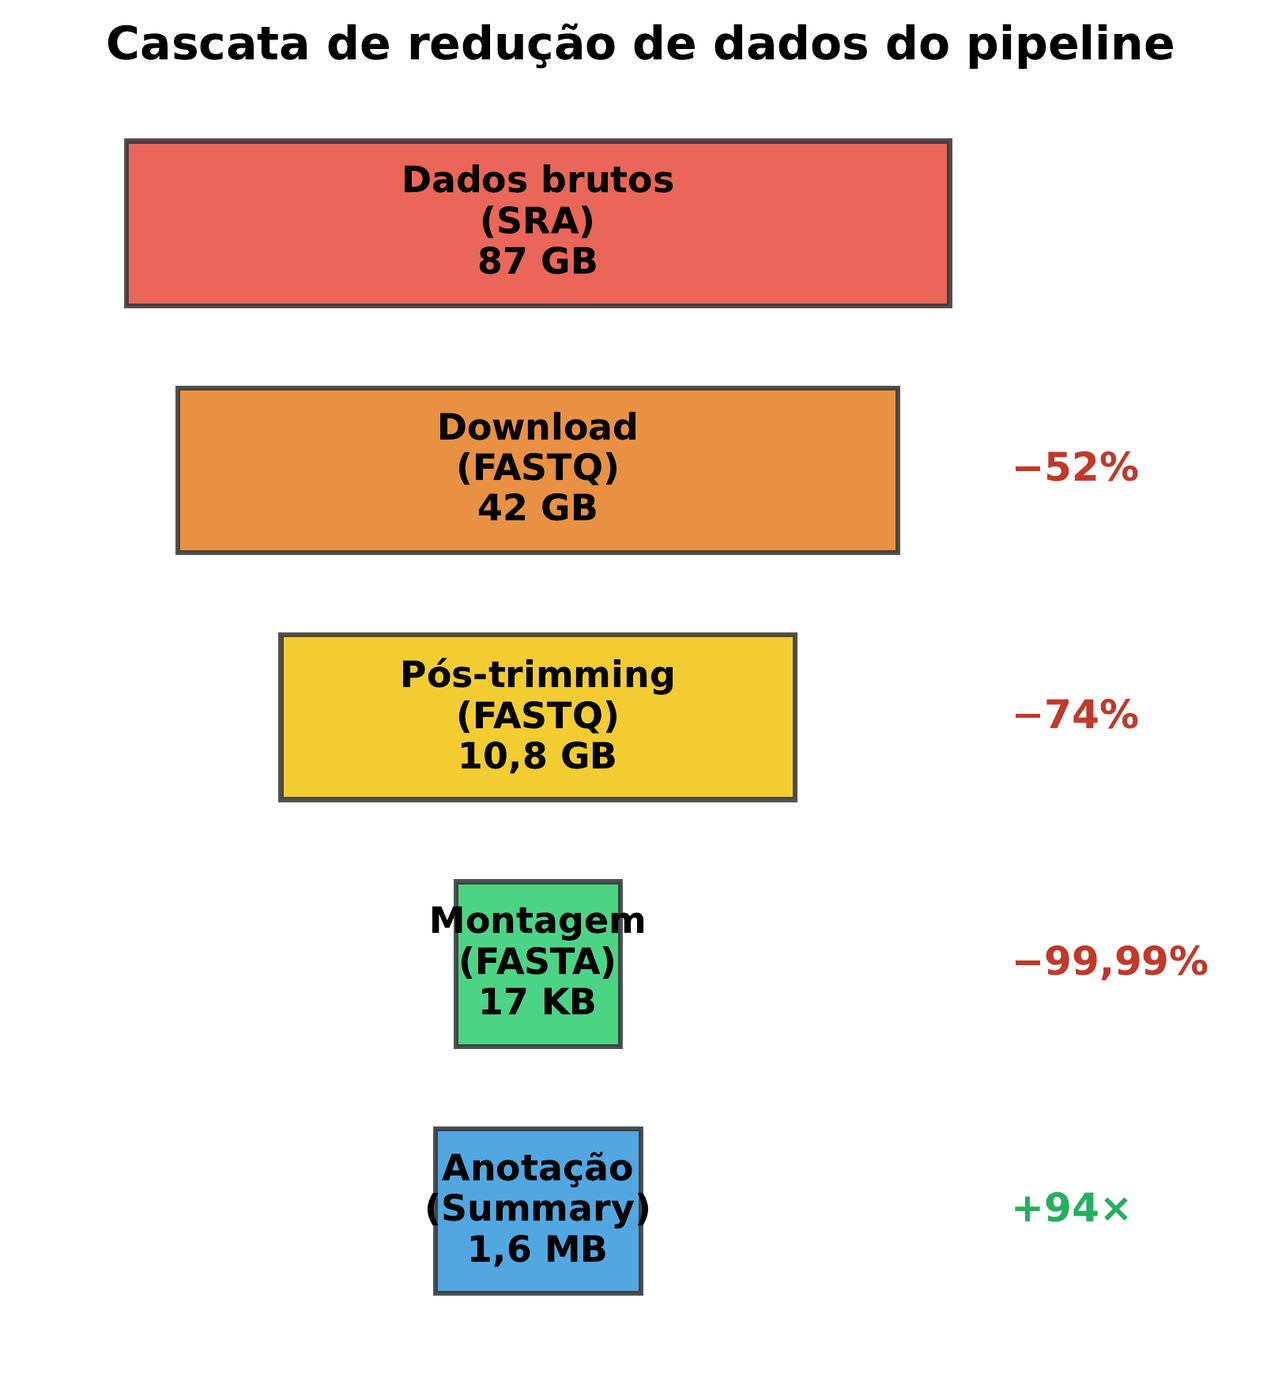
\includegraphics[width=0.85\textwidth]{imagens/funil_reducao_dados.png}
    \caption{Cascata de redução de dados ao longo do pipeline: de 87~GB de FASTQ bruto até 17~KB de genoma circularizado --- uma redução de aproximadamente 5 milhões de vezes.}
    \label{fig:funil_reducao}
\end{figure}

\subsection{Pico de Armazenamento e Custo Computacional}

Um aspecto frequentemente negligenciado em pipelines bioinformáticos é o \textbf{consumo de armazenamento durante a execução}, que pode ser significativamente maior que o tamanho dos resultados finais. Isso ocorre porque as etapas intermediárias geram arquivos temporários volumosos (FASTQs descomprimidos, arquivos de cache) que são consumidos pelas etapas seguintes e depois descartados.

No caso da execução para a arara-azul-de-lear, o pico de uso de disco foi de \textbf{27~GB} no diretório de trabalho, dominado pela etapa SRA\_DOWNLOAD (23~GB de FASTQs descomprimidos e cache \texttt{.sra}). Em contraste, ao final da execução, os resultados úteis ocupam apenas \textbf{$\sim$67~MB} em \texttt{results/}. Os arquivos intermediários podem ser removidos com o comando \texttt{nextflow clean}, liberando o espaço ocupado. Essa diferença de $\sim$400$\times$ entre o pico de armazenamento e os resultados finais é uma característica importante a considerar ao dimensionar a infraestrutura.

\textbf{Custo computacional em hardware doméstico.} Todo o pipeline foi executado em um notebook pessoal com processador de 4 núcleos, 16~GB de RAM e disco SSD convencional. Os requisitos computacionais reais observados foram:

\begin{itemize}
    \item \textbf{Processamento:} 56,7 minutos de tempo total (\textit{wall-clock}), com pico de uso de 4 threads durante a conversão SRA e o trimming. Nenhuma etapa exigiu processamento de alto desempenho --- o processo mais intensivo (NOVOPlasty) utilizou apenas 1 thread.
    \item \textbf{Armazenamento:} 27~GB de pico no diretório de trabalho, reduzidos a $\sim$67~MB de resultados finais após limpeza dos arquivos temporários. Um disco com pelo menos 50~GB livres é suficiente com margem de segurança.
    \item \textbf{Memória RAM:} pico de 11,1~GB durante a montagem com NOVOPlasty, dentro dos 16~GB disponíveis. Um computador com 8~GB de RAM pode apresentar lentidão nessa etapa, mas não é impedido de executá-la.
    \item \textbf{Rede:} o download do arquivo SRA ($\sim$11~GB) foi o principal consumidor de banda, com duração variável conforme a velocidade da conexão.
\end{itemize}

Esses requisitos modestos demonstram que \textbf{a montagem e anotação de mitogenomas não exige infraestrutura computacional especializada}. Qualquer computador pessoal de categoria intermediária, com 16~GB de RAM, disco SSD e acesso à internet, é capaz de executar o pipeline completo em menos de uma hora. Essa acessibilidade é particularmente relevante para estudantes e grupos de pesquisa com recursos limitados, que podem reproduzir integralmente os resultados deste trabalho sem investimento adicional em hardware.

\subsection{Caminho Crítico e Otimização Implementada}

O \textbf{caminho crítico} de um pipeline --- ou seja, a sequência de etapas dependentes que determina o tempo mínimo de execução --- é: SRA\_PILOT $\rightarrow$ SRA\_DOWNLOAD $\rightarrow$ TRIM\_GALORE $\rightarrow$ NOVOPLASTY $\rightarrow$ MITOS2 $\rightarrow$ COMPILE\_SUMMARY. Etapas que executam em paralelo, como o FASTQC (que processa os mesmos FASTQs que o Trim Galore ao mesmo tempo), \textbf{não adicionam tempo ao caminho crítico}, exceto quando excedem a duração da etapa paralela. No caso observado, o FASTQC (7,6~min) completou antes do Trim Galore (12,2~min) e, portanto, não impactou o tempo total.

A análise do caminho crítico revela que \textbf{81,1\% do tempo total} (46 de 56,7~min) é consumido por apenas duas etapas: download/conversão SRA (33,8~min) e trimming (12,2~min). A montagem em si --- o objetivo central do pipeline --- leva apenas 4,5 minutos (8,0\%), demonstrando que o gargalo real não é computacional, mas de transferência e transformação de dados.

A partir dessa análise, foi identificada e implementada uma otimização concreta. A análise da sub-amostragem interna do NOVOPlasty (Seção~5.7.3) revelou que apenas 22,93\% das reads foram efetivamente utilizadas na montagem. Isso indica que o limite anteriormente definido (50 milhões de reads) era excessivamente conservador: com 25 milhões de reads, a cobertura estimada seria de $\sim$150$\times$ --- ainda 3$\times$ acima do mínimo recomendado na literatura \cite{dierckxsens2017}. Com base nessa evidência, o limite máximo do módulo Pilot QC foi reduzido de 50 milhões para 25 milhões de reads, diminuindo proporcionalmente o tempo de download, conversão e trimming. A estimativa de tempo total com essa otimização é de $\sim$35 minutos --- uma redução de 38\% em relação à execução observada --- sem comprometer a qualidade da montagem.

\subsection{Síntese da Análise de Desempenho}

A análise de desempenho revelou três conclusões principais sobre o comportamento computacional do pipeline:

\textbf{O gargalo é I/O, não processamento.} Das sete etapas do pipeline, a montagem do mitogenoma --- objetivo central do trabalho --- consome apenas 8\% do tempo total (4,5~min). O restante é dominado por operações de transferência e transformação de dados: o download e conversão do SRA representam 59,6\% (33,8~min) e o trimming responde por 21,5\% (12,2~min). Em termos práticos, isso significa que melhorias na velocidade de rede ou na estratégia de amostragem têm impacto muito maior no tempo total do que otimizações no algoritmo de montagem.

\textbf{A etapa de trimming justifica seu custo.} Apesar de consumir 12 minutos, o trimming não é dispensável: 81,4\% das reads continham sequências de adaptadores que, se mantidas, poderiam gerar extensões quiméricas no grafo do NOVOPlasty. Os 12 minutos investidos previnem falhas de circularização que exigiriam re-execução completa do pipeline --- um custo muito superior.

\textbf{Sem as estratégias implementadas no pipeline, a montagem de um mitogenoma a partir de dados públicos seria inviável em hardware doméstico.} O dataset original de \textit{A.~leari} (SRR28399504) contém 118,5 milhões de pares de leituras, que, quando convertidos para o formato FASTQ, ocupam aproximadamente 87~GB de espaço em disco. Carregar e processar esse volume na íntegra --- como seria necessário em uma abordagem manual sem truncamento --- exigiria centenas de gigabytes de armazenamento temporário (leitura, escrita intermediária e saída), além de memória RAM proporcional ao volume de dados nos estágios de trimming e montagem. Um notebook convencional com 16~GB de RAM e 256~GB de SSD simplesmente não comportaria essa carga; seria necessário recorrer a um servidor dedicado ou a uma infraestrutura de computação em nuvem.

O pipeline resolve esse problema por meio de uma cadeia de reduções progressivas que viabilizam a execução em hardware modesto. O \textbf{Pilot QC} analisa uma amostra mínima (500 mil leituras, $\sim$500~MB) e calcula exatamente quantas leituras são necessárias para atingir a cobertura-alvo, evitando o download do dataset inteiro. O \textbf{truncamento} reduz o volume de 87~GB para $\sim$21~GB (apenas 25 milhões de pares). O \textbf{trimming} remove adaptadores e bases de baixa qualidade, reduzindo para $\sim$10,8~GB de dados úteis. Finalmente, o \textbf{NOVOPlasty} sub-amostra internamente e opera apenas sobre as leituras que alinham à semente, consumindo uma fração do total. O resultado: de 87~GB de dados brutos, o pipeline extrai um mitogenoma de \textbf{17~KB} --- uma redução de aproximadamente 5 milhões de vezes.

Essa cadeia de decisões é o que torna possível executar o ciclo completo --- do dado bruto público ao mitogenoma anotado com 14 categorias de entregáveis --- em aproximadamente 35 minutos, em um notebook com 4 núcleos e 16~GB de RAM, sem necessidade de infraestrutura especializada. A viabilidade em hardware doméstico é particularmente relevante para estudantes de graduação e pesquisadores em instituições com recursos computacionais limitados, que de outra forma dependeriam de acesso a servidores ou clusters para realizar análises genômicas.

% A Figura~\ref{fig:tempo_etapas} já apresenta o detalhamento do tempo por etapa.

\section{Discussão sobre a Robustez da Abordagem}

A execução bem-sucedida do pipeline para duas espécies distintas --- uma ave (Psittaciformes) e um peixe (Perciformes) ---, utilizando datasets de plataformas diferentes (HiSeq X Ten e NovaSeq X Plus), demonstra a generalização da abordagem. A obtenção de genomas circularizados em ambos os casos, com o conjunto completo de 37 genes identificados no caso anotado, valida tanto o fluxo de montagem quanto a integração de ferramentas.

A cobertura de 306$\times$ obtida para \textit{A.~leari} com apenas 0,17\% de leituras mitocondriais em 20 milhões de pares demonstra que o DNA mitocondrial é eficientemente recuperado pelo NOVOPlasty mesmo quando representa uma fração diminuta do total de dados, confirmando as observações da literatura \cite{dierckxsens2017}.

A combinação metodológica adotada neste trabalho --- NOVOPlasty para montagem e MITOS2 para anotação --- corresponde ao padrão predominante na literatura recente de genômica mitocondrial, empregada em estudos abrangendo desde 213 mitogenomas de lagartos \cite{zhan2024} até espécies individuais de peixes \cite{kundu2024}, arraias \cite{guerreiro2025} e invertebrados \cite{shi2024,tao2024}. Essa convergência metodológica independente --- em que grupos de pesquisa de diferentes países, trabalhando com táxons distintos, adotam as mesmas ferramentas --- constitui uma validação externa da abordagem e reforça a confiabilidade das escolhas implementadas no pipeline.

A lógica iterativa de montagem com re-seeding automático e múltiplos k-mers mostrou-se eficaz, circularizando na primeira tentativa (k-mer 39) para \textit{A.~leari} e na primeira tentativa (k-mer 33) para \textit{D.~bifasciatus}. Essa robustez é particularmente relevante para cenários em que a \textit{seed} disponível é de uma espécie distante, ou quando regiões repetitivas dificultam a circularização.

O módulo Pilot QC foi validado por meio de execução isolada do script \texttt{pilot\_qc.sh} sobre uma subamostra de 100.000 leituras de \textit{A.~leari}, extraída do dataset SRR28399504. A análise piloto detectou qualidade Q30 de 86,2\%, taxa de adaptador de 66,4\% e fração mitocondrial estimada de 0,17\% (via correspondência de k-mers com a semente cox1). Com esses valores, a recomendação automática foi de 36 milhões de leituras para atingir 500$\times$ de cobertura --- resultado coerente com os 306$\times$ efetivamente obtidos com 20 milhões de leituras na execução principal. A configuração de produção do perfil \texttt{a\_leari} não define \texttt{sra\_max\_reads}, ativando o Pilot QC automaticamente em execuções futuras. Essa funcionalidade é particularmente valiosa para pesquisadores trabalhando com espécies pouco caracterizadas, onde não há estimativa prévia da fração mitocondrial.

Em comparação com os trabalhos relacionados, o pipeline desenvolvido apresenta vantagens claras em termos de reprodutibilidade, portabilidade e acessibilidade computacional. Enquanto o MitoHiFi \cite{ulianosilva2023} utiliza Conda para gerenciamento de dependências, sujeito a variações de ambiente, e o MITObim \cite{hahn2013} e o GetOrganelle \cite{jin2020} dependem de configuração manual, o pipeline aqui proposto encapsula todas as ferramentas em containers Docker com versões pinadas e orquestra sua execução via Nextflow, garantindo resultados idênticos em qualquer ambiente. Adicionalmente, as soluções existentes não incorporam mecanismos de redução automática do volume de dados, pressupondo que o usuário disponha de infraestrutura com armazenamento e memória suficientes para processar datasets completos --- requisito que exclui a maioria dos computadores pessoais. O pipeline aqui proposto, ao integrar o Pilot QC e o truncamento adaptativo, elimina essa barreira e permite que o ciclo completo --- do dado bruto ao mitogenoma anotado --- seja executado em um notebook convencional. A adição da Fase 2 (anotação funcional com MITOS2 e geração automática de entregáveis em formato GenBank) vai além do que a maioria dos pipelines de montagem de organelas oferece, cobrindo o ciclo completo desde o dado bruto até a submissão ao banco de dados.

Os resultados metodológicos apresentados neste capítulo demonstram que o pipeline é funcional, eficiente e acessível. O capítulo seguinte dedica-se integralmente à espécie-alvo deste trabalho --- a arara-azul-de-lear ---, explorando em profundidade o mitogenoma obtido, sua organização gênica e as implicações para a conservação da espécie.

% ============================================================================
% CAPÍTULO 6 — O MITOGENOMA DA ARARA-AZUL-DE-LEAR
% ============================================================================

\chapter{O Mitogenoma da Arara-azul-de-lear}
\label{cap:mitogenoma}

Este capítulo apresenta a caracterização biológica completa do mitogenoma da arara-azul-de-lear (\textit{Anodorhynchus leari}), montado e anotado pelo pipeline descrito nos capítulos anteriores. A análise abrange a contextualização da espécie, a composição nucleotídica, os genes codificadores de proteínas, os RNAs transportadores e ribossomais, a organização gênica comparada e as implicações para a conservação.

\section{A Espécie}
\label{sec:especie}

A arara-azul-de-lear (\textit{Anodorhynchus leari} Bonaparte, 1856) é um psitacídeo de grande porte endêmico do bioma Caatinga, no nordeste do Brasil. Pertencente à ordem Psittaciformes, família Psittacidae, gênero \textit{Anodorhynchus}, a espécie compartilha o gênero com apenas duas outras araras: a arara-azul-grande (\textit{A.~hyacinthinus}) e a provavelmente extinta arara-azul-pequena (\textit{A.~glaucus}) \cite{collar1997}. A descoberta formal da espécie para a ciência ocorreu em 1856, mas sua área de ocorrência em vida livre só foi localizada por Helmut Sick em 1978, no Raso da Catarina, norte do estado da Bahia \cite{sick1979}.

A distribuição geográfica de \textit{A.~leari} é extremamente restrita. A espécie ocorre em uma área de aproximadamente 1.500~km² no semiárido baiano, com núcleos populacionais concentrados nas regiões de Toca Velha e Serra Branca, nos municípios de Canudos, Jeremoabo e Euclides da Cunha \cite{icmbio2022}. Os indivíduos nidificam em paredões de arenito, onde escavam cavidades para reprodução, e se alimentam predominantemente de frutos de palmeira licuri (\textit{Syagrus coronata}), estabelecendo uma relação ecológica de forte dependência \cite{sick1979,icmbio2022}.

A população atual é estimada em aproximadamente 1.700 indivíduos em vida livre \cite{icmbio2022}, representando uma recuperação significativa em relação aos cerca de 200 indivíduos registrados na década de 1980 \cite{sick1979,icmbio2022}. A espécie é classificada como \textbf{Em Perigo} (EN) pela União Internacional para a Conservação da Natureza (IUCN) e consta no Plano de Ação Nacional para a Conservação da Arara-azul-de-lear (PAN Arara-azul-de-lear) \cite{icmbio2022}.

As principais ameaças à sobrevivência da espécie incluem: (i)~o tráfico ilegal de filhotes, que historicamente representou o fator mais crítico de redução populacional; (ii)~a degradação e fragmentação do habitat, particularmente pela remoção de palmeiras licuri para extração de cera e uso da terra para pecuária; (iii)~a baixa variabilidade genética resultante do gargalo populacional histórico, que aumenta a vulnerabilidade a doenças e reduz a capacidade adaptativa; e (iv)~a área de distribuição extremamente restrita, que torna a espécie vulnerável a eventos estocásticos como secas prolongadas ou epizootias.

Neste contexto, a genômica de conservação utiliza dados moleculares para subsidiar decisões de manejo de espécies ameaçadas. O sequenciamento do mitogenoma completo da arara-azul-de-lear representa uma contribuição direta para esse campo, fornecendo marcadores moleculares para identificação forense, avaliação de diversidade genética e análises filogenéticas.

\missingfigure{Mapa da distribuição geográfica da arara-azul-de-lear no nordeste da Bahia}

\missingfigure{Fotografia da arara-azul-de-lear em ambiente natural}

\section{Caracterização Geral do Mitogenoma}
\label{sec:caracterizacao}

O mitogenoma da arara-azul-de-lear possui 16.986 pares de bases (bp) e topologia circular, conforme esperado para genomas mitocondriais de metazoários. O genoma contém 37 genes --- 13 genes codificadores de proteínas (CDS), 22 genes de RNA transportador (tRNA), 2 genes de RNA ribossomal (rRNA) --- além da região controle (D-loop).

A composição nucleotídica do mitogenoma é apresentada na Tabela~\ref{tab:composicao_nt}.

\begin{table}[H]
\centering
\caption{Composição nucleotídica do mitogenoma de \textit{A.~leari}.}
\label{tab:composicao_nt}
\begin{tabular}{@{}lrr@{}}
\toprule
\textbf{Base} & \textbf{Quantidade} & \textbf{Proporção (\%)} \\
\midrule
A & 5.153 & 30,3 \\
T & 3.978 & 23,4 \\
G & 2.372 & 14,0 \\
C & 5.474 & 32,2 \\
\midrule
Total & 16.986 & 100,0 \\
\bottomrule
\end{tabular}
\end{table}

O conteúdo GC do mitogenoma é de 46,2\%. Os índices de assimetria composicional refletem o viés replicativo característico de genomas mitocondriais:

\begin{itemize}
    \item \textbf{AT-skew} = $\frac{A - T}{A + T}$ = $\frac{5.153 - 3.978}{5.153 + 3.978}$ = +0,129 (excesso de adenina na fita pesada);
    \item \textbf{GC-skew} = $\frac{G - C}{G + C}$ = $\frac{2.372 - 5.474}{2.372 + 5.474}$ = $-$0,395 (excesso de citosina na fita pesada).
\end{itemize}

Esses valores são consequência da replicação assimétrica do DNA mitocondrial. Durante a replicação, a fita pesada (H-strand) permanece em estado de fita simples por um período prolongado, exposta a desaminação espontânea de citosina para uracila (e, portanto, timina) e de adenina para hipoxantina (equivalente a guanina). Esse viés mutacional resulta na depleção de citosina e adenina na fita pesada, gerando os padrões de AT-skew positivo e GC-skew negativo observados \cite{boore1999}.

A comparação dos índices de assimetria com outras espécies analisadas na literatura demonstra a consistência desses padrões. A raia \textit{Potamotrygon leopoldi} apresenta AT-skew de +0,13 e GC-skew de $-$0,40 \cite{guerreiro2025}, valores praticamente idênticos aos de \textit{A.~leari}. Já espécies filogeneticamente mais distantes exibem variações: o lagarto \textit{Calotes taeniops} apresenta AT-skew de +0,052 e GC-skew de $-$0,277 \cite{kundu2024}, enquanto a salamandra \textit{Desmognathus japonicus} apresenta AT-skew de $-$0,001 e GC-skew de $-$0,273 \cite{hong2024}. A similaridade entre \textit{A.~leari} e \textit{P.~leopoldi} ilustra a convergência de pressões seletivas sobre a composição nucleotídica mitocondrial, mesmo entre linhagens evolutivamente distantes.

O conteúdo gênico do mitogenoma é sumarizado na Tabela~\ref{tab:conteudo_genico}.

\begin{table}[H]
\centering
\caption{Conteúdo gênico do mitogenoma de \textit{A.~leari}.}
\label{tab:conteudo_genico}
\begin{tabular}{@{}clp{8cm}@{}}
\toprule
\textbf{Categoria} & \textbf{Quantidade} & \textbf{Detalhes} \\
\midrule
CDS & 13 & ND1--6, ND4L, COX1--3, ATP6, ATP8, CYTB \\
\addlinespace
tRNA & 22 & Um por aminoácido; leucina e serina possuem dois isoaceptores cada \\
\addlinespace
rRNA & 2 & 12S rRNA (rrnS, 970 bp) e 16S rRNA (rrnL, 1.572 bp) \\
\addlinespace
D-loop & 2 segmentos & OH\_0 (262 bp) e OH\_1 (47 bp) \\
\bottomrule
\end{tabular}
\end{table}

A região controle (D-loop) é uma região não codificante que contém os promotores para replicação e transcrição do DNA mitocondrial \cite{boore1999}. Por não sofrer as mesmas pressões seletivas que os genes codificadores, apresenta a maior taxa de variação entre todas as regiões do mitogenoma, sendo particularmente útil para estudos de diversidade genética intrapopulacional.

\begin{figure}[H]
    \centering
    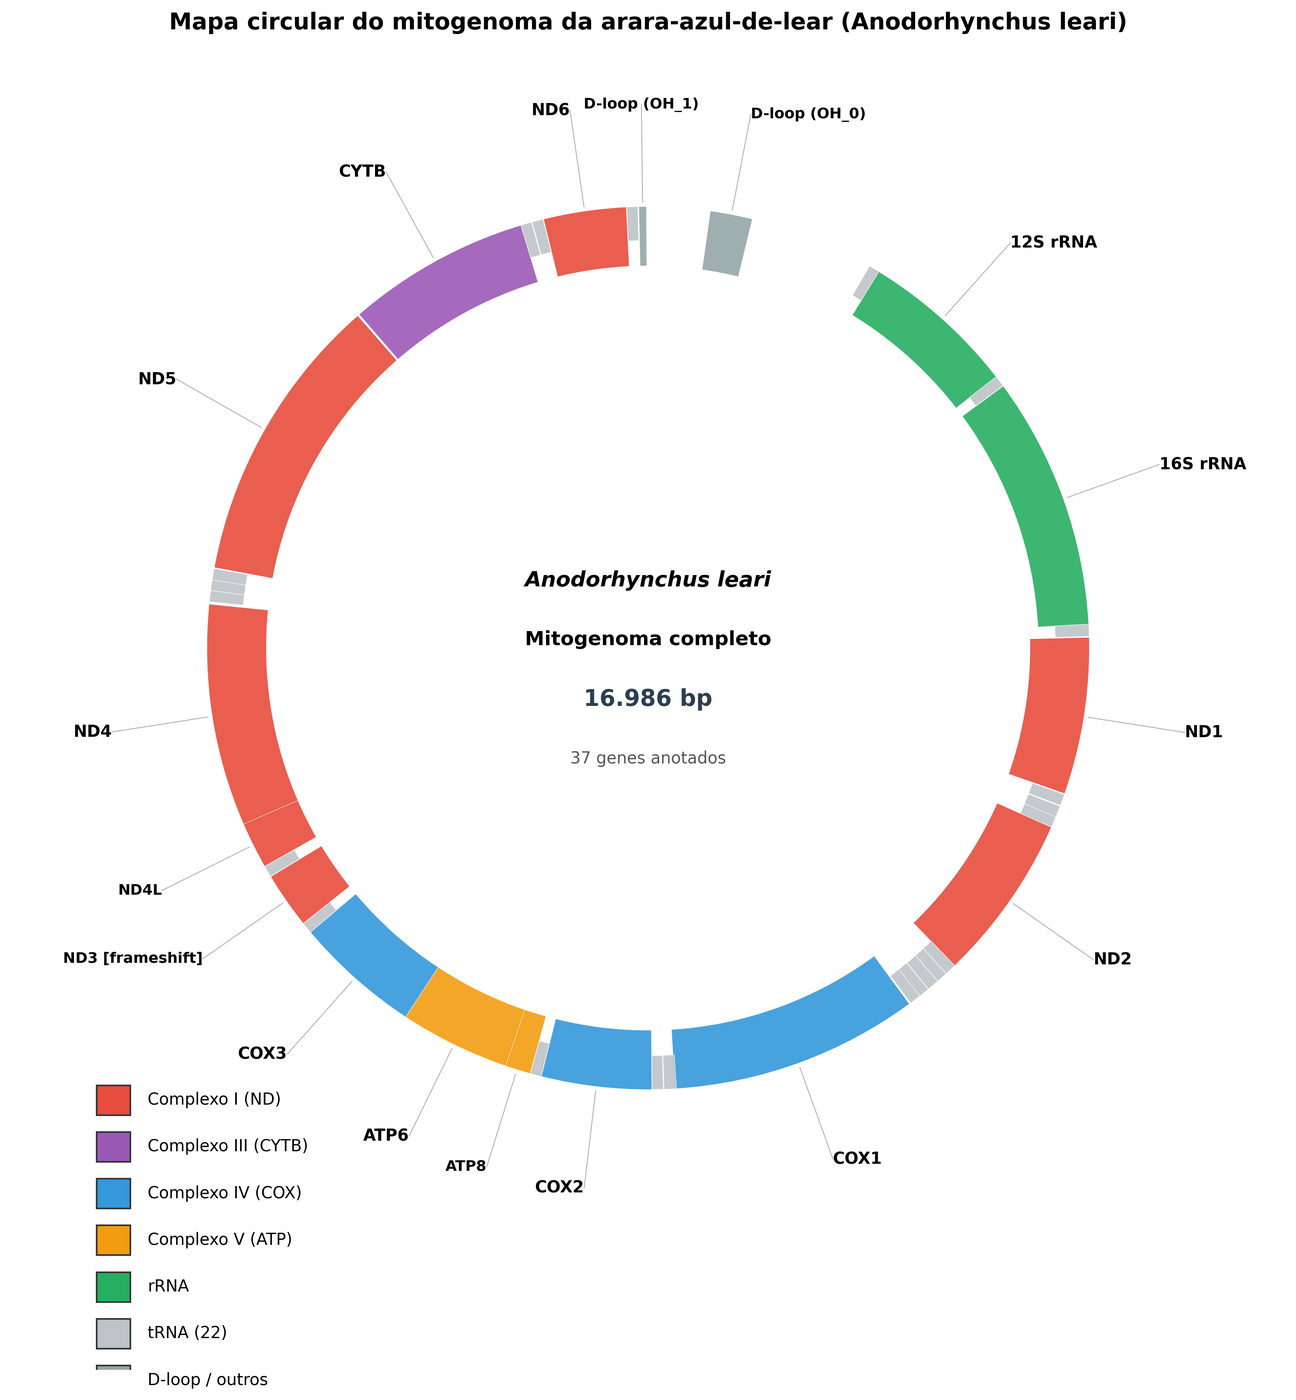
\includegraphics[width=0.70\textwidth]{imagens/mapa_circular_mitogenoma.png}
    \caption{Mapa circular do mitogenoma da arara-azul-de-lear (\textit{A.~leari}, 16.986~bp), com a posição dos 37 genes coloridos por categoria funcional. Gerado automaticamente pelo pipeline via Biopython GenomeDiagram.}
    \label{fig:mapa_circular_leari}
\end{figure}

\section{Genes Codificadores de Proteínas}
\label{sec:cds}

O mitogenoma de \textit{A.~leari} codifica 13 genes de proteínas, correspondentes a subunidades de quatro dos cinco complexos da cadeia respiratória mitocondrial:

\begin{itemize}
    \item \textbf{Complexo I} (NADH desidrogenase): ND1, ND2, ND3, ND4, ND4L, ND5, ND6 --- sete subunidades;
    \item \textbf{Complexo III} (citocromo $b$): CYTB --- uma subunidade;
    \item \textbf{Complexo IV} (citocromo $c$ oxidase): COX1, COX2, COX3 --- três subunidades;
    \item \textbf{Complexo V} (ATP sintase): ATP6, ATP8 --- duas subunidades.
\end{itemize}

O Complexo II (succinato desidrogenase) é ausente em todos os genomas mitocondriais de metazoários, sendo codificado exclusivamente pelo genoma nuclear. Dos 13 genes, 12 são codificados na fita pesada (H-strand), enquanto o ND6 é o único gene codificador na fita leve (L-strand) --- padrão universal em mitogenomas aviários.

A Tabela~\ref{tab:codons} apresenta os códons de início e parada, bem como os tamanhos de cada gene codificador.

\begin{table}[H]
\centering
\caption{Códons de início e parada dos genes codificadores de proteínas de \textit{A.~leari}.}
\label{tab:codons}
\begin{tabular}{@{}llrrr@{}}
\toprule
\textbf{Gene} & \textbf{Início} & \textbf{Parada} & \textbf{Tamanho (bp)} & \textbf{Tamanho (aa)} \\
\midrule
ND1  & ATG & TA(+A)  & 974   & 324 \\
ND2  & ATA & TAA     & 1.041 & 347 \\
COX1 & GTG & AGG     & 1.548 & 516 \\
COX2 & ATG & TAA     & 684   & 228 \\
ATP8 & ATG & TAA     & 168   & 56  \\
ATP6 & ATG & TAA     & 684   & 228 \\
COX3 & ATG & T(+AA)  & 784   & 261 \\
ND4L & ATG & TAA     & 297   & 99  \\
ND4  & ATG & T(+AA)  & 1.378 & 459 \\
ND5  & ATA & TAA     & 1.809 & 603 \\
CYTB & ATG & TAA     & 1.140 & 380 \\
ND6  & ATG & TAG     & 513   & 171 \\
ND3  & ATA & GAA     & 349*  & 118* \\
\bottomrule
\end{tabular}
\begin{flushleft}
\small{* Valores referentes ao gene completo incluindo a região de \textit{frameshift} (ver Seção~\ref{subsec:nd3_frameshift}).}
\end{flushleft}
\end{table}

Três padrões são observados nos códons dos genes codificadores:

(i) O códon de início ATG é o mais frequente, utilizado por 9 dos 13 genes. Os códons alternativos ATA (ND2, ND5, ND3) e GTG (COX1) são aceitos no código genético mitocondrial de vertebrados. As mitocôndrias utilizam um código genético ligeiramente diferente do padrão universal: ATA codifica metionina (em vez de isoleucina), TGA codifica triptofano (em vez de parada), e AGA/AGG funcionam como códons de parada (em vez de arginina) \cite{anderson1981,boore1999}. Esse código corresponde à Tabela 2 do NCBI (\textit{Vertebrate Mitochondrial Code}).

(ii) Três genes (ND1, COX3 e ND4) apresentam códons de parada incompletos, terminando em ``TA'' ou ``T''. Esse fenômeno é consequência do processamento do mRNA policistrônico mitocondrial: a clivagem pós-transcricional do transcrito primário, seguida de poliadenilação, completa o códon de parada TAA pela adição de resíduos de adenina na extremidade 3' do mRNA \cite{anderson1981}.

(iii) O gene ND6, único na fita leve, utiliza o códon de parada TAG, distinto do padrão TAA predominante nos demais genes.

\paragraph*{Análise Ka/Ks.}

A razão Ka/Ks (também denominada dN/dS) é a razão entre substituições não sinônimas ($K_a$, que alteram o aminoácido) e substituições sinônimas ($K_s$, silenciosas). Valores de Ka/Ks $< 1$ indicam seleção purificadora (pressão para manter a sequência proteica), Ka/Ks $> 1$ indica seleção positiva (favorecimento de mudanças), e Ka/Ks $= 1$ indica evolução neutra.

Um padrão universal emerge da literatura: todos os 13 genes codificadores mitocondriais apresentam Ka/Ks $< 1$ em \textbf{todos} os táxons analisados --- aves, répteis, peixes, moluscos, insetos, crustáceos e cnidários \cite{zhan2024,guerreiro2025,shi2024,ye2024,kundu2024,alboasud2024,zhou2024,tao2024}. O gene COX1 é consistentemente o mais conservado (Ka/Ks entre 0,02 e 0,07), refletindo as restrições funcionais severas sobre a subunidade catalítica do Complexo IV. Em contraste, o ATP8 é o mais variável (Ka/Ks entre 0,5 e 0,8), compatível com seu pequeno tamanho e menor número de sítios funcionalmente críticos. Em Planorbidae (caramujos), \citeonline{tao2024} reportaram Ka/Ks $> 1$ para ATP8 em alguns gêneros, sugerindo seleção positiva pontual.

Para \textit{A.~leari}, a conservação de COX1 é evidenciada pela alta identidade com \textit{A.~hyacinthinus}. A comparação direta de Ka/Ks entre as duas espécies de \textit{Anodorhynchus} constitui uma perspectiva futura relevante para identificar genes sob pressão seletiva diferencial.

\paragraph*{Uso de Códons (RSCU).}

O \textit{Relative Synonymous Codon Usage} (RSCU) quantifica a preferência entre códons sinônimos para um mesmo aminoácido. Em genomas mitocondriais, há um viés sistemático em favor de códons com adenina ou timina na terceira posição. \citeonline{shi2024} demonstraram que esse viés é direcionado por seleção natural, e não apenas por pressão mutacional. O padrão é menos extremo em vertebrados, porém detectável \cite{kundu2024,guerreiro2025}. A construção de tabelas de RSCU para \textit{A.~leari} constitui uma perspectiva futura que permitirá comparações detalhadas com outros Psittaciformes.

\subsection{O \textit{Frameshift} do ND3: Uma Assinatura Evolutiva Conservada}
\label{subsec:nd3_frameshift}

O gene ND3 apresenta uma característica incomum compartilhada por aves, tartarugas e crocodilianos: um \textit{frameshift} (mudança de quadro de leitura) que divide o gene em dois quadros abertos de leitura (ORFs) sobrepostos.

\paragraph*{Descoberta.}

O \textit{frameshift} do ND3 foi identificado por \citeonline{mindell1998} em 52 espécies de aves e 10 espécies de tartarugas. Após o nucleotídeo 174 a partir do códon de início, uma inserção de um único nucleotídeo desloca o quadro de leitura em +1. Isso divide o gene em dois ORFs: o primeiro codifica 58 aminoácidos (posições 1--174) e o segundo codifica aproximadamente 59 aminoácidos no quadro deslocado. O MITOS2 anotou essa estrutura como \texttt{nad3\_0} (174~bp) e \texttt{nad3\_1} (180~bp) com sobreposição de 5~bp no sítio de deslizamento --- resultado plenamente consistente com a literatura.

\paragraph*{Mecanismo molecular.}

Duas hipóteses explicam como a proteína ND3 funcional é traduzida apesar da mudança de quadro de leitura:

\begin{enumerate}[label=(\roman*)]
    \item \textbf{\textit{Programmed} +1 \textit{ribosomal frameshifting} (+1 PRF)}: o ribossomo desliza um nucleotídeo adiante (+1) no sítio de \textit{frameshift}, continuando a tradução no novo quadro de leitura. Esse mecanismo difere do $-$1 PRF descrito em retrovírus como HIV e RSV \cite{jacks1988}, onde sequências escorregadias (\textit{slippery sequences}) do tipo X\_XXY\_YYH e pseudonós a jusante induzem o deslizamento reverso \cite{brierley1995,atkins2016}. No +1 PRF, a pausa ribossomal ocorre pela escassez de tRNAs raros complementares ao códon no sítio A, favorecendo cineticamente o deslizamento para frente \cite{harger2002}.

    \item \textbf{Edição pós-transcricional do mRNA}: o nucleotídeo extra é removido por edição do mRNA antes da tradução, restaurando o quadro de leitura original. Evidências para esse mecanismo foram obtidas em estudos de cDNA de tartarugas \cite{russell2008}.
\end{enumerate}

Ambos os mecanismos podem coexistir como redundância funcional, garantindo a produção da proteína ND3 funcional.

\begin{figure}[H]
    \centering
    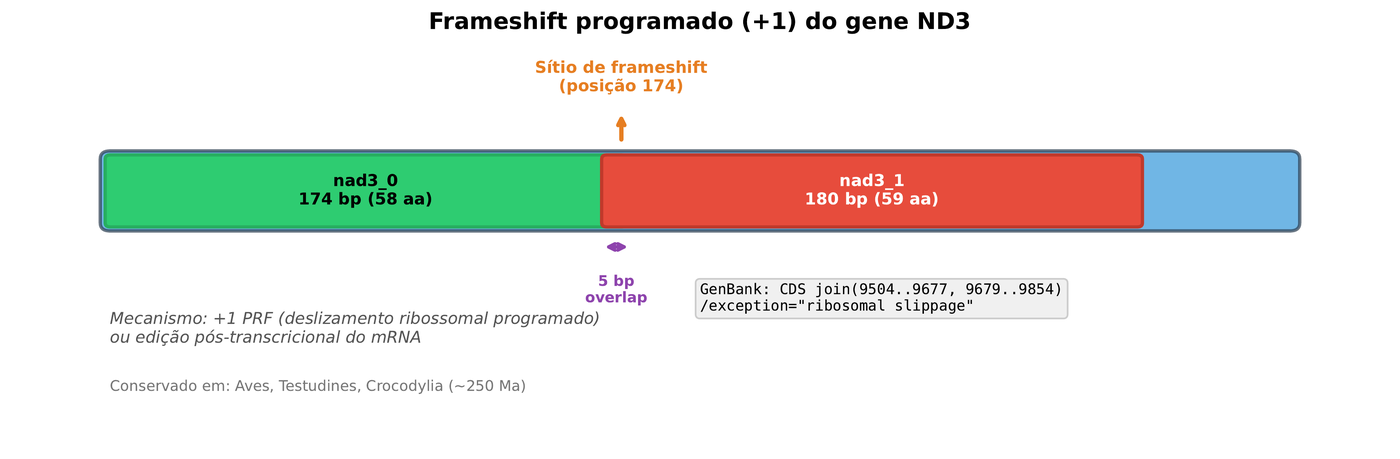
\includegraphics[width=0.85\textwidth]{imagens/frameshift_nd3.png}
    \caption{Diagrama esquemático do \textit{frameshift} do gene ND3: a inserção de um nucleotídeo na posição 174 desloca o quadro de leitura em +1, dividindo o gene em dois ORFs (\texttt{nad3\_0} e \texttt{nad3\_1}).}
    \label{fig:frameshift_nd3}
\end{figure}

\paragraph*{Distribuição taxonômica.}

O \textit{frameshift} do ND3 está presente em todas as aves (Aves), tartarugas (Testudines) e crocodilianos (Crocodylia). \citeonline{russell2008} identificaram inserções de \textit{frameshift} em seis sítios separados em três genes (\textit{nad3}, \textit{nad4l}, \textit{cob}) em tartarugas, e documentaram que \textit{Chelodina parkeri} apresenta reassociação de códon de parada --- o primeiro caso registrado em DNA mitocondrial de vertebrados. O \textit{frameshift} está ausente em mamíferos, anfíbios e na maioria dos peixes. Sua distribuição mapeia o clado Archelosauria (Aves + Crocodylia + Testudines), sugerindo uma única origem há aproximadamente 250 milhões de anos.

\paragraph*{Resultado em \textit{A.~leari}.}

O MITOS2 detectou automaticamente o \textit{frameshift} como \texttt{nad3\_0} + \texttt{nad3\_1}, consistente com a anotação de \textit{A.~hyacinthinus} (NC\_082165.1), onde o ND3 é anotado como:

\begin{lstlisting}
CDS   join(9504..9677,9679..9854)
      /gene="ND3"
\end{lstlisting}

O script \texttt{gff2genbank\allowbreak.py} do pipeline utiliza \texttt{join()} com o qualificador \texttt{/exception=\allowbreak"ribosomal\allowbreak{} slippage"}, conforme as diretrizes do NCBI para submissão ao GenBank.

\section{RNAs Transportadores e Ribossomais}
\label{sec:trna_rrna}

O mitogenoma de \textit{A.~leari} contém 22 genes de tRNA, codificando transportadores para os 20 aminoácidos padrão. Os aminoácidos leucina e serina possuem dois isoaceptores cada: tRNA-Leu(UUR) e tRNA-Leu(CUN); tRNA-Ser(UCN) e tRNA-Ser(AGY). Dos 22 tRNAs, 14 são codificados na fita pesada e 8 na fita leve. A Tabela~\ref{tab:trna} apresenta as características de cada tRNA.

\begin{longtable}{@{}llcl@{}}
\caption{Genes de tRNA do mitogenoma de \textit{A.~leari}.}
\label{tab:trna} \\
\toprule
\textbf{tRNA} & \textbf{Tamanho (bp)} & \textbf{Anticódon} & \textbf{Aminoácido} \\
\midrule
\endfirsthead
\caption[]{Genes de tRNA do mitogenoma de \textit{A.~leari} (continuação).} \\
\toprule
\textbf{tRNA} & \textbf{Tamanho (bp)} & \textbf{Anticódon} & \textbf{Aminoácido} \\
\midrule
\endhead
\bottomrule
\endfoot
tRNA-Phe     & 67 & GAA & Fenilalanina \\
tRNA-Val     & 69 & TAC & Valina \\
tRNA-Leu(UUR) & 74 & TAA & Leucina \\
tRNA-Ile     & 71 & GAT & Isoleucina \\
tRNA-Gln     & 70 & TTG & Glutamina \\
tRNA-Met     & 68 & CAT & Metionina \\
tRNA-Trp     & 70 & TCA & Triptofano \\
tRNA-Ala     & 68 & TGC & Alanina \\
tRNA-Asn     & 73 & GTT & Asparagina \\
tRNA-Cys     & 66 & GCA & Cisteína \\
tRNA-Tyr     & 70 & GTA & Tirosina \\
tRNA-Ser(UCN) & 75 & TGA & Serina \\
tRNA-Asp     & 68 & GTC & Aspartato \\
tRNA-Lys     & 68 & TTT & Lisina \\
tRNA-Gly     & 68 & TCC & Glicina \\
tRNA-Arg     & 69 & TCG & Arginina \\
tRNA-His     & 68 & GTG & Histidina \\
tRNA-Ser(AGY) & 65 & GCT & Serina \\
tRNA-Leu(CUN) & 70 & TAG & Leucina \\
tRNA-Thr     & 67 & TGT & Treonina \\
tRNA-Pro     & 68 & TGG & Prolina \\
tRNA-Glu     & 68 & TTC & Glutamato \\
\end{longtable}

Os tRNAs mitocondriais variam de 65 a 75~bp (média de 69~bp). Todos apresentam a estrutura secundária canônica em trevo (\textit{cloverleaf}), predita por RNAplot/ViennaRNA \cite{lorenz2011} a partir dos modelos de covariância do MITOS2, com uma exceção notável: o tRNA-Ser(AGY) carece do braço DHU, adotando uma conformação simplificada em formato ``D''. Essa ausência é conservada em \textbf{todos} os metazoários há mais de 600 milhões de anos e foi reportada em todos os 15 artigos analisados na revisão de literatura: corais \cite{wei2024}, bivalves \cite{li2023,kartavtsev2024}, estrelas-do-mar \cite{alboasud2024}, afídeos \cite{shi2024}, caramujos planorbídeos \cite{tao2024}, tubarões \cite{ye2024}, raias \cite{guerreiro2025}, lagartos \cite{zhan2024}, anfíbios \cite{hong2024} e teleósteos \cite{kundu2024}. A estrutura simplificada é reconhecida pelo ribossomo mitocondrial por mecanismos alternativos de reconhecimento.

\begin{figure}[H]
    \centering
    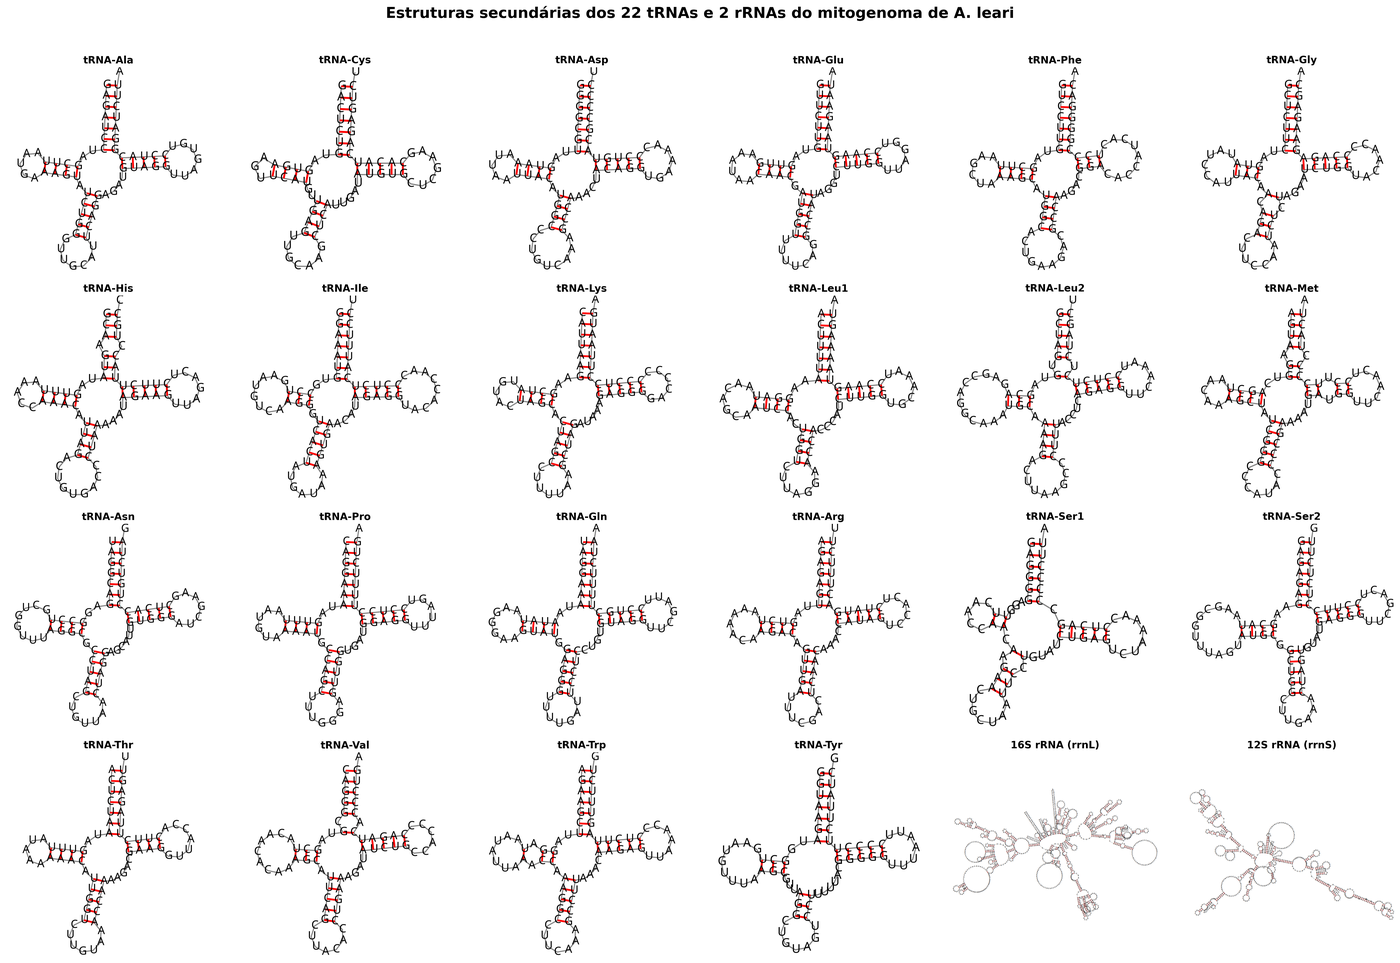
\includegraphics[width=\textwidth]{imagens/painel_trna_rrna.png}
    \caption{Estruturas secundárias em trevo dos 22 tRNAs e 2 rRNAs do mitogenoma de \textit{A.~leari}, preditas pelo MITOS2/RNAplot. O tRNA-Ser(AGY) carece do braço DHU, conformação conservada em todos os metazoários.}
    \label{fig:trna_estruturas}
\end{figure}

O mitogenoma contém dois genes de rRNA: o 12S (rrnS, 970~bp) e o 16S (rrnL, 1.572~bp), localizados entre os genes tRNA-Phe e tRNA-Leu(UUR), separados pelo tRNA-Val. Essa organização é invariável em todos os Psittaciformes. Os ribossomos mitocondriais (mitorribossomos) possuem coeficiente de sedimentação de 55S, com a subunidade menor (28S) contendo o rRNA 12S e a subunidade maior (39S) contendo o rRNA 16S.

\section{Organização Gênica e Comparação com \textit{A.~hyacinthinus}}
\label{sec:organizacao_genica}

A ordem gênica do mitogenoma de \textit{A.~leari} segue o padrão neognata (\textit{standard avian gene order}), descrito por \citeonline{desjardins1990}:

\begin{footnotesize}
\noindent
D-loop --- trnF --- rrnS --- trnV --- rrnL --- trnL2 --- nad1 --- trnI --- trnQ\textsuperscript{(--)} --- trnM --- nad2 --- trnW --- trnA\textsuperscript{(--)} --- trnN\textsuperscript{(--)} --- trnC\textsuperscript{(--)} --- trnY\textsuperscript{(--)} --- cox1 --- trnS2\textsuperscript{(--)} --- trnD --- cox2 --- trnK --- atp8 --- atp6 --- cox3 --- trnG --- nad3 --- trnR --- nad4l --- nad4 --- trnH --- trnS1 --- trnL1 --- nad5 --- cob --- trnT --- trnP\textsuperscript{(--)} --- nad6\textsuperscript{(--)} --- trnE\textsuperscript{(--)} --- D-loop
\end{footnotesize}

\noindent onde o sobrescrito \textsuperscript{(--)} indica genes codificados na fita leve (L-strand).

A comparação direta com o congênere \textit{A.~hyacinthinus} (NC\_082165.1, 16.999~bp) é apresentada na Tabela~\ref{tab:comparacao_hyacinthinus}.

\begin{table}[H]
\centering
\caption{Comparação entre os mitogenomas de \textit{A.~leari} e \textit{A.~hyacinthinus}.}
\label{tab:comparacao_hyacinthinus}
\begin{tabular}{@{}lll@{}}
\toprule
\textbf{Característica} & \textbf{\textit{A.~leari}} & \textbf{\textit{A.~hyacinthinus}} \\
\midrule
Tamanho total   & 16.986 bp & 16.999 bp \\
Diferença       & ---       & $\Delta$ 13 bp \\
CDS             & 13        & 13 \\
tRNAs           & 22        & 22 \\
rRNAs           & 2         & 2 \\
Ordem gênica    & Padrão aviário & Padrão aviário \\
\textit{Frameshift} ND3 & Presente & Presente \\
CDS na fita L   & ND6       & ND6 \\
\bottomrule
\end{tabular}
\end{table}

A diferença de apenas 13~bp ($\sim$0,08\%) entre os dois mitogenomas reflete a divergência recente entre as espécies, consistente com estimativas de separação no Plioceno \cite{tavares2006}. Os mitogenomas são sintênicos --- apresentam a mesma organização estrutural, sem rearranjos detectáveis.

A alta similaridade entre os dois congêneres possui implicações diretas para a conservação. \citeonline{ye2024} demonstraram que o gene COX1 isoladamente é insuficiente para discriminar espécies proximamente relacionadas de tubarões do gênero \textit{Scoliodon}, sendo necessária a análise de múltiplos genes ou do mitogenoma completo. Essa observação é diretamente relevante para \textit{Anodorhynchus}: com apenas 13~bp de divergência total, marcadores conservados como COX1 e CYTB podem ser insuficientes para a discriminação forense entre \textit{A.~leari} e \textit{A.~hyacinthinus}.

\paragraph*{O D-loop como marcador diferencial.}

A região controle (D-loop) apresenta a maior variação inter e intraespecífica no mitogenoma. Em tubarões \textit{Scoliodon}, \citeonline{ye2024} demonstraram a utilidade dessa região para discriminação interespecífica. Em raias \textit{Potamotrygon}, \citeonline{guerreiro2025} identificaram repetições em tandem na região controle, enquanto em afídeos, \citeonline{shi2024} observaram variação geográfica no comprimento do D-loop (650--1.109~bp). A comparação detalhada dos D-loops de \textit{A.~leari} e \textit{A.~hyacinthinus} --- incluindo domínios conservados (\textit{Conserved Central Domains}, CCDs), blocos de sequência conservados (\textit{Conserved Sequence Blocks}, CSBs) e repetições em tandem --- constitui uma perspectiva futura estratégica para a identificação de marcadores forenses diferenciadores entre as duas espécies.

\missingfigure{Diagrama de sintenia comparando mitogenomas de A. leari e A. hyacinthinus}

\section{Implicações para a Conservação}
\label{sec:implicacoes_conservacao}

A disponibilidade do mitogenoma completo de \textit{A.~leari} abre perspectivas concretas para a conservação da espécie, subsidiando aplicações em três frentes complementares: identificação forense, avaliação de diversidade genética e filogeografia.

Antes de discutir essas aplicações, é necessário definir os conceitos fundamentais da genética de conservação empregados nesta análise:

\begin{itemize}
    \item \textbf{Haplótipo}: variante genética definida por mutações específicas, compartilhada por um grupo de indivíduos que a herdou de um ancestral comum. No DNA mitocondrial, cada haplótipo representa uma linhagem materna distinta.

    \item \textbf{Diversidade nucleotídica} ($\pi$): proporção média de nucleotídeos diferentes entre dois indivíduos de uma mesma população. Valores baixos indicam baixa variação genética, típica de populações que sofreram gargalos populacionais.

    \item \textbf{Depressão endogâmica} (\textit{inbreeding depression}): redução da aptidão (\textit{fitness}) decorrente do acúmulo de alelos recessivos deletérios quando indivíduos aparentados se reproduzem --- inevitável em populações pequenas.

    \item \textbf{Filogeografia}: estudo da distribuição geográfica de linhagens genéticas, integrando filogenética molecular e biogeografia.

    \item \textbf{Relógio molecular}: estimativa de tempos de divergência entre espécies com base na taxa de acúmulo de mutações ao longo do tempo.

    \item \textbf{Especiação}: processo pelo qual uma população ancestral se divide em espécies distintas, reprodutivamente isoladas.
\end{itemize}

\paragraph*{Identificação forense.}

O tráfico ilegal de filhotes constitui uma das principais ameaças à arara-azul-de-lear. Um paralelo pode ser traçado com a raia de água doce \textit{Potamotrygon leopoldi} \cite{guerreiro2025}, cujo mitogenoma de 17.504~bp revelou sinais de seleção positiva nos genes ND1, ND4, ND5, COX1 e COX2, associados à adaptação ao ambiente de água doce. O mitogenoma completo viabiliza a criação de marcadores de DNA \textit{barcoding} \cite{hebert2003} para identificação inequívoca da espécie. Os genes COX1 (1.548~bp) e CYTB (1.140~bp) representam a primeira abordagem para laboratórios forenses. Todavia, o COX1 isoladamente é insuficiente para espécies proximamente relacionadas \cite{ye2024}. Modelos de aprendizado de máquina (\textit{Random Forest}, SVM, MLP) com AUC $>$ 0,90, treinados com os 13 genes codificadores, poderiam distinguir \textit{A.~leari} de \textit{A.~hyacinthinus} --- aplicáveis a ovos, penas, tecidos ou indivíduos em cativeiro.

\paragraph*{Avaliação de diversidade genética.}

A população de \textit{A.~leari} sofreu um severo gargalo demográfico entre as décadas de 1970 e 1990, quando foi reduzida a aproximadamente 200 indivíduos \cite{sick1979,icmbio2022}. Gargalos dessa magnitude reduzem drasticamente a variabilidade genética, aumentando a vulnerabilidade a doenças e a depressão endogâmica. A sequência mitocondrial completa permite o sequenciamento da região D-loop de múltiplos indivíduos para estimar o número de haplótipos circulantes, a diversidade nucleotídica ($\pi$) e a estrutura populacional entre os núcleos de Toca Velha e Serra Branca. Esses dados constituem insumos diretos para o Plano de Ação Nacional \cite{icmbio2022} e para decisões de manejo, como translocações entre populações e programas de reprodução em cativeiro.

\paragraph*{Filogeografia e evolução do gênero.}

O mitogenoma completo possibilita análises filogenéticas multigênicas robustas dentro de Psittaciformes. A divergência de 13~bp em relação a \textit{A.~hyacinthinus} pode ser utilizada para calibrar relógios moleculares e estimar tempos de divergência, contribuindo para a compreensão da biogeografia histórica do gênero \textit{Anodorhynchus} e dos processos de especiação na Caatinga \cite{tavares2006}.

\section{Disponibilidade dos Dados}
\label{sec:disponibilidade}

Os dados gerados neste trabalho estão disponíveis nos seguintes formatos:

\begin{itemize}
    \item \textbf{GenBank Flat File} (\texttt{A\_leari.gbk}): formato padrão do NCBI, pronto para submissão. Contém todos os 37 genes anotados, com \texttt{join()} e \texttt{/exception="ribosomal slippage"} para o \textit{frameshift} do ND3.

    \item \textbf{Feature Table} (\texttt{A\_leari.tbl}) e \textbf{FASTA formatado} (\texttt{A\_leari.fsa}): para processamento pela ferramenta \texttt{table2asn} do NCBI.

    \item \textbf{Repositório GitHub}: todo o código-fonte --- Dockerfiles, módulos Nextflow, scripts de análise e configurações de perfil --- está disponível publicamente para reprodutibilidade completa \cite{wilkinson2016}.
\end{itemize}

A disponibilidade pública contribui para a democratização do acesso à bioinformática, permitindo que outros grupos de pesquisa reproduzam as análises ou apliquem o pipeline a outras espécies --- aves, peixes, invertebrados ou qualquer metazoário --- necessitando apenas de um acesso SRA e uma sequência-semente de gene mitocondrial. A generalização do pipeline foi verificada pela execução bem-sucedida em dois táxons distintos (Psittaciformes e Perciformes), reforçando a aderência aos princípios FAIR (\textit{Findable, Accessible, Interoperable, and Reusable}).

% ===================================================================
% Capítulo 7 — Considerações Finais
% ===================================================================
\chapter{CONSIDERAÇÕES FINAIS}
\label{cap:consideracoes}

\begin{figure}[H]
    \centering
    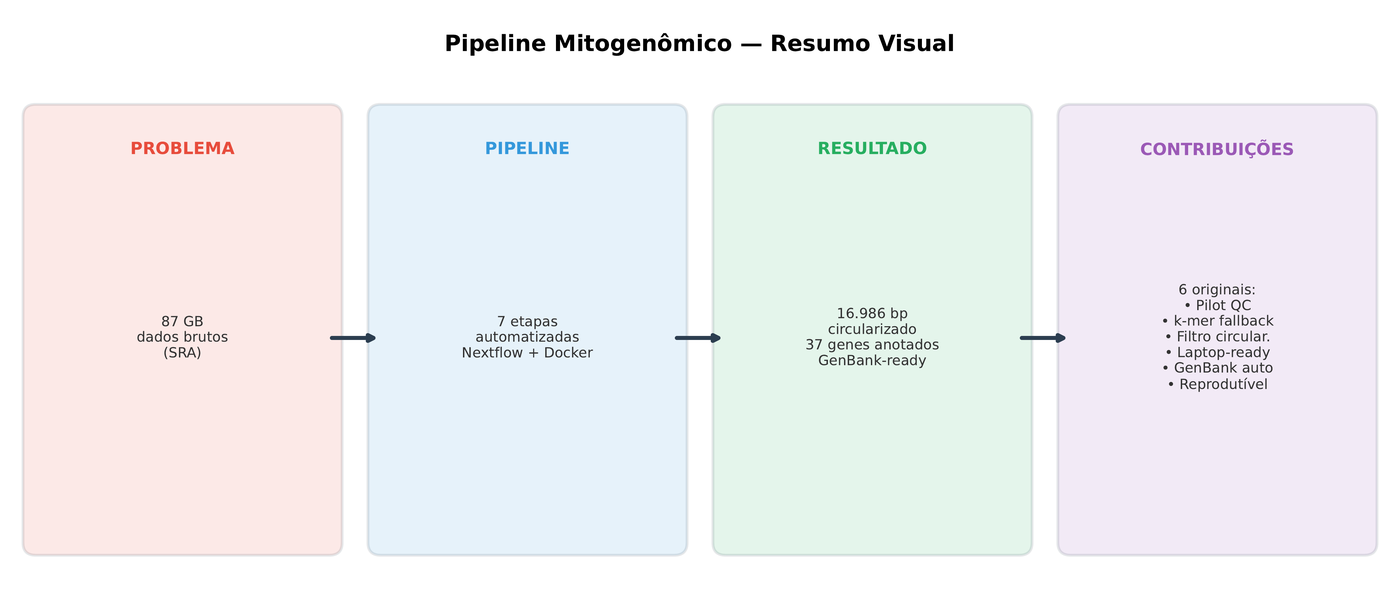
\includegraphics[width=\textwidth]{imagens/infografico_resumo.png}
    \caption{Infográfico-resumo do trabalho: do problema inicial (87~GB de dados brutos), passando pelas 7 etapas do pipeline, até o resultado final (16.986~bp circularizado, 37 genes, GenBank-ready) e as 6 contribuições originais.}
    \label{fig:infografico_resumo}
\end{figure}

O presente trabalho teve como objetivo propor e implementar um pipeline de bioinformática voltado à montagem e anotação funcional de genomas mitocondriais, concebido segundo princípios de automação, reprodutibilidade, ciência aberta e acessibilidade computacional. A integração de sete ferramentas consolidadas --- SRA-Toolkit, FastQC, Trim Galore com Cutadapt, NOVOPlasty, MITOS2, ViennaRNA e Biopython \cite{cock2009} --- em um fluxo containerizado (Docker) e orquestrado por meio do Nextflow constitui a principal contribuição metodológica desta proposta, ao oferecer uma solução transparente, portável e replicável para análises genômicas.

Um resultado particularmente significativo deste trabalho é a demonstração de que a montagem e anotação completa de mitogenomas a partir de dados públicos é viável em hardware doméstico. O dataset original utilizado totaliza 87\,GB de leituras brutas --- volume que, sem as estratégias de redução implementadas, exigiria centenas de gigabytes de armazenamento temporário e servidores dedicados. A cadeia de reduções progressivas incorporada ao pipeline (Pilot QC, truncamento adaptativo, \textit{trimming}) reduz esse volume em aproximadamente 5 milhões de vezes, viabilizando a execução em notebooks com 16\,GB de RAM em menos de uma hora. Essa acessibilidade é especialmente relevante para estudantes, pesquisadores iniciantes e instituições com recursos computacionais limitados, que anteriormente dependeriam de acesso a servidores ou \textit{clusters} para realizar análises genômicas equivalentes.

Do ponto de vista biológico, o pipeline foi aplicado com sucesso à montagem do mitogenoma da arara-azul-de-lear (16.986\,bp circularizado, 306$\times$ de cobertura, 37 genes identificados) e à espécie de validação \textit{Diploprion bifasciatus} (circularizado). Conforme detalhado no Capítulo~\ref{cap:mitogenoma}, a caracterização completa do mitogenoma da arara-azul-de-lear revelou composição nucleotídica, organização gênica e assinaturas moleculares (como o \textit{frameshift} do ND3) consistentes com a espécie congênere \textit{A. hyacinthinus}, confirmando a qualidade da montagem e a aplicabilidade dos dados para estudos de conservação, identificação forense e filogeografia.

Dentre as contribuições originais do pipeline, destacam-se:

\begin{enumerate}[label=(\roman*)]
    \item o módulo Pilot QC, que determina automaticamente o volume de dados necessário para atingir a cobertura desejada, evitando processamento desnecessário e viabilizando a execução em computadores com armazenamento limitado;
    \item a cadeia de reduções progressivas (Pilot QC $\rightarrow$ truncamento $\rightarrow$ \textit{trimming}) que transforma 87\,GB de dados brutos em um mitogenoma de 17\,KB, eliminando a necessidade de servidores dedicados;
    \item a lógica iterativa de montagem com \textit{re-seeding} automático e múltiplos \textit{k-mers};
    \item a geração automática de estruturas secundárias de tRNAs e rRNAs via RNAplot/ViennaRNA, funcionalidade anteriormente restrita à interface web do MITOS2;
    \item a conversão automática para GenBank Flat File com tratamento do \textit{frameshift} do ND3; e
    \item a compilação automática de 14 categorias de entregáveis em pasta organizada.
\end{enumerate}

Apesar de seu potencial, algumas limitações precisam ser reconhecidas. O sucesso da montagem depende da qualidade da \textit{seed} inicial e da profundidade de cobertura dos dados de sequenciamento. A anotação do MITOS2, embora automatizada, pode requerer curadoria manual em casos de estruturas gênicas atípicas (como o \textit{frameshift} do ND3). Adicionalmente, o tamanho dos \textit{containers} Docker ($\sim$2--4\,GB por imagem) pode representar uma barreira em ambientes com espaço de armazenamento limitado.

Como perspectivas futuras, propõem-se:

\begin{enumerate}[label=(\roman*)]
    \item a validação da montagem de \textit{D.~bifasciatus} por BLAST contra a referência PZ143763.1 do GenBank;
    \item a submissão do mitogenoma da arara-azul-de-lear ao GenBank;
    \item a integração de análises filogenéticas automáticas ao pipeline (MAFFT + RAxML/\allowbreak IQ-TREE);
    \item a geração automática de tabelas de RSCU (\textit{Relative Synonymous Codon Usage}) e de razão Ka/Ks para análise de pressão seletiva sobre os genes codificadores --- análises que se tornaram padrão em estudos recentes de genômica mitocondrial \cite{zhan2024,kundu2024,shi2024};
    \item a integração de tRNAscan-SE como módulo opcional de verificação dos tRNAs preditos pelo MITOS2, seguindo a prática consolidada na literatura;
    \item a geração de gráficos de sintenia comparativa entre espécies congêneres; e
    \item a publicação do pipeline no nf-core como recurso comunitário.
\end{enumerate}

Em síntese, o pipeline desenvolvido representa uma contribuição metodológica significativa para a bioinformática de organelas, ao unir rigor técnico, aplicabilidade biológica e boas práticas de reprodutibilidade computacional. Mais do que atender a um caso de estudo específico, constitui um recurso com potencial de ser reutilizado, adaptado e expandido por diferentes grupos de pesquisa, colaborando para a consolidação de uma ciência mais transparente, padronizada e sustentável.


% ============================================================================
% ELEMENTOS PÓS-TEXTUAIS
% ============================================================================
\postextual

% ---- REFERÊNCIAS ----
\bibliography{references}

\end{document}
